\RequirePackage{silence}
\WarningFilter{latex}{Font shape}
\documentclass{ucao}
\usepackage{amsmath}
\usepackage{tikz}
\usepackage{float}
\usepackage{longtable}
\usetikzlibrary{shapes.geometric, arrows.meta, positioning, fit, backgrounds, shadows.blur, calc}
\addbibresource{biblio.bib}

\defbibfilter{web}{type=misc or type=online}

\title{Conception et réalisation d'une unité mobile, autonome et connectée de pré-traitement du soja : \\ Projet SMART-SOJA BÉNIN}

%Maitre de mémoire
\maitrememoire{Dr DIDAVI K. B. Audace}
\titremaitrememoire{Enseignant}

%Maitre de stage
\maitrestage{Mme AHISSOU Kyrielle \\ Mme SOSSOUKPE Carine}
\titremaitrestage{Encadrantes techniques à QOTTO Bénin}

% Jury non encore constitué — décommenter et compléter une fois les noms connus
%\jury{
%\begin{description}
%\item[Président~:]    Prénom {\bfseries NOM}, Grade, Institution
%\item[Examinateur~:]  Prénom {\bfseries NOM}, Grade, Institution
%\item[Rapporteur~:]   Prénom {\bfseries NOM}, Grade, Institution
%\end{description}
%}

\logouniversite{images/ucao}
\scalelogouniversite{0.45}
\logoecole{images/egei}
\scalelogoecole{0.15}

\author{Elisa Christelle LOKO \and Dodji Virgile TCHIDEHOU}

\date{Session Juin 2026}

\cycle{Licence Professionnelle}
\filiere{Sciences et Technologies}
\option{Informatique Industrielle et Maintenance}

% Correction de la Table des Figures (Standard Académique)
\makeatletter
\renewcommand{\l@figure}{\@dottedtocline{1}{1.5em}{3.2em}} % Augmente la largeur pour éviter les troncatures
\renewcommand{\l@table}{\@dottedtocline{1}{1.5em}{3.2em}}
\makeatother


\begin{document}

% -------------------------------------------------------
% Suppression des pages blanches entre chapitres (mode oneside)
\let\cleardoublepage\clearpage
% -------------------------------------------------------

\maketitle


% ================= SECTIONS PRÉLIMINAIRES =================
\frontmatter



\shorttoc{Sommaire}{0}

\chapter*{Dédicaces}
\addcontentsline{toc}{chapter}{Dédicaces}
\chaptermark{Dédicaces}

% ==================== DÉDICACE — Elisa Christelle LOKO ====================

\begin{flushright}
\normalsize

\textit{Je dédie ce mémoire avant tout à Dieu Tout-Puissant,}\\
\textit{pour Sa grâce, Sa protection et la force qu’Il m’a accordées}\\
\textit{tout au long de mon parcours.}\\[0.2cm]

\textit{À mes très chers parents,}\\
\textit{aucun mot ne saurait exprimer toute la gratitude, l’amour et le respect que je vous porte. Merci pour vos sacrifices, votre soutien indéfectible, vos conseils et vos prières qui m'ont accompagnée tout au long de ce parcours. Ce mémoire est le fruit de vos efforts, de votre patience et de la confiance que vous avez toujours placée en moi. Que ce travail soit pour vous une source de fierté et le témoignage de ma profonde reconnaissance.}\\[0.2cm]

\textit{À mes chers frères,}\\
\textit{aucun mot ne saurait traduire toute ma reconnaissance pour les sacrifices, le soutien et l’amour dont vous avez fait preuve à mon égard tout au long de mon parcours universitaire. Merci d’avoir toujours cru en moi, de m'avoir soutenue dans les moments difficiles et de m’avoir permis d’avancer avec confiance.}\\
\textit{Ce mémoire est aussi le reflet de vos efforts et de votre présence à mes côtés. Que Dieu vous bénisse abondamment.}\\[0.2cm]

\textit{À tous mes proches, amis, enseignants et formateurs,}\\
\textit{pour leurs conseils, leurs encouragements et leur accompagnement tant sur le plan académique qu’humain.}\\[0.2cm]

\textit{Enfin, à toutes les personnes qui ont contribué à la réalisation de ce travail, j’adresse mes sincères remerciements et ma profonde gratitude.}\\[0.4cm]

\textbf{--- Elisa Christelle LOKO}

\end{flushright}

\vspace*{\fill}

% ==================== PAGE SUIVANTE ====================
\newpage

% ==================== DÉDICACE — Dodji Virgile TCHIDEHOU ====================

\vspace*{\fill}

\begin{flushright}
\normalsize

\textit{Je dédie ce mémoire avant tout à Dieu Tout-Puissant,}\\
\textit{pour Sa grâce infinie, Sa protection}\\
\textit{et la force qu'Il m'a accordées tout au long de ce parcours.}\\[0.8cm]

\textit{À la mémoire de mon père,}\\[0.3cm]
\textit{dont l'absence demeure une douleur,}\\
\textit{mais dont les valeurs, les conseils et les sacrifices}\\
\textit{continuent de guider mes pas chaque jour.}\\
\textit{Ce travail est le fruit de l'éducation qu'il a semée en moi.}\\
\textit{Puisse-t-il reposer en paix.}\\[0.8cm]

\textit{À ma mère, à mes frères et sœurs,}\\[0.3cm]
\textit{pour leur amour, leurs encouragements, leurs sacrifices,}\\
\textit{leur présence et leur soutien constant,}\\
\textit{malgré les difficultés.}\\[0.8cm]

\textit{À toute ma famille,}\\[0.3cm]
\textit{pour l'affection, les encouragements}\\
\textit{et les nombreux soutiens apportés tout au long de mon parcours.}\\[0.8cm]

\textit{Enfin, à toutes les personnes qui ont soutenu ma formation}\\
\textit{et contribué à la réalisation de ce mémoire,}\\
\textit{je témoigne ma profonde gratitude.}\\[1cm]

\textbf{--- Dodji Virgile TCHIDEHOU}

\end{flushright}

\vspace*{\fill}

\chapter*{Remerciements}
\addcontentsline{toc}{chapter}{Remerciements}
\chaptermark{Remerciements}

Au terme de ce mémoire de fin de cycle, nous exprimons notre profonde gratitude à toutes les personnes qui ont contribué, de près ou de loin, à l’aboutissement de ce travail. Nous remercions d’abord les autorités de l’Université Catholique de l’Afrique de l’Ouest, de l’UCAO-UUC et de l’École de Génie Électrique et Informatique pour le cadre de formation mis à notre disposition. Nous adressons également nos remerciements à l’ensemble du corps enseignant, technique et administratif pour la qualité de l’encadrement reçu tout au long de notre parcours.

Nous remercions particulièrement \textbf{Dr DIDAVI K. B. Audace}, notre maître de mémoire, pour sa disponibilité, ses orientations scientifiques, ses conseils et sa rigueur dans le suivi de ce travail. Nos remerciements vont aussi à \textbf{Mme ALAHASSA Gwladys}, Directrice Générale de \textbf{QOTTO Bénin}, ainsi qu’à \textbf{Mme AHISSOU Kyrielle} et \textbf{Mme SOSSOUKPE Carine}, nos encadrantes techniques, pour leur accompagnement, leur disponibilité et l’appui apporté à la réalisation du prototype.

Nous remercions également le personnel de \textbf{QOTTO Bénin}, les responsables et techniciens de \textbf{Sèmè City Open Park} ayant facilité certaines opérations de fabrication, les membres du jury pour l’honneur qu’ils nous font en acceptant d’évaluer ce travail, nos camarades de promotion pour leur collaboration, ainsi que nos familles respectives pour leur soutien constant et leurs sacrifices.

\chapter*{Sigles et abréviations}
\addcontentsline{toc}{chapter}{Sigles et abréviations}
\chaptermark{Sigles et abréviations}

\begin{sigleslist}
    \item[ADC] Analog-to-Digital Converter (Convertisseur Analogique-Numérique)
    \item[API] Application Programming Interface (Interface de Programmation d'Application)
    \item[BMS] Battery Management System (Système de gestion de batterie)
    \item[CAO] Conception Assistée par Ordinateur
    \item[DHT] Digital Humidity and Temperature
    \item[DRC] Design Rule Check (Vérification des règles de conception)
    \item[EDA] Electronic Design Automation (Conception Électronique Assistée par Ordinateur)
    \item[ESP32] Microcontrôleur avec Wi-Fi et Bluetooth intégré (SOC)
    \item[FreeRTOS] Free Real-Time Operating System
    \item[GDIZ] Glo-Djigbé Industrial Zone
    \item[GEI] Génie Électrique et Informatique
    \item[GPRS] General Packet Radio Service
    \item[GSM] Global System for Mobile Communications
    \item[HR] Humidité Relative
    \item[I2C] Inter-Integrated Circuit
    \item[IFU] Identifiant Fiscal Unique
    \item[IoT] Internet of Things (Internet des objets)
    \item[JSON] JavaScript Object Notation
    \item[LCD] Liquid Crystal Display (Écran à Cristaux Liquides)
    \item[LiFePO4] Lithium Fer Phosphate
    \item[LPWAN] Low-Power Wide-Area Network
    \item[MOSFET] Metal-Oxide-Semiconductor Field-Effect Transistor
    \item[MPPT] Maximum Power Point Tracking (Suivi du point de puissance maximale)
    \item[MQTT] Message Queuing Telemetry Transport
    \item[PCB] Printed Circuit Board (Circuit Imprimé)
    \item[PWM] Pulse Width Modulation (Modulation par Largeur d'Impulsion)
    \item[RCCM] Registre du Commerce et du Crédit Mobilier
    \item[RTC] Real-Time Clock (Horloge Temps Réel)
    \item[RTOS] Real-Time Operating System (Système d'Exploitation Temps Réel)
    \item[SARL] Société à Responsabilité Limitée
    \item[SCOP] Sèmè City Open Park
    \item[SD] Secure Digital
    \item[SHS] Solar Home System (Système Solaire Domestique)
    \item[SPI] Serial Peripheral Interface
    \item[TCXO] Temperature-Compensated Crystal Oscillator
    \item[TGX] Tropical Glycine Cross (Variété de soja)
    \item[UART] Universal Asynchronous Receiver-Transmitter
    \item[UCAO] Université Catholique de l'Afrique de l'Ouest
    \item[UUC] Unité Universitaire à Cotonou
    \item[WSN] Wireless Sensor Network (Réseau de Capteurs Sans Fil)
\end{sigleslist}


\newpage
\listoffigures
\listoftables

\chapter*{Résumé}
\addcontentsline{toc}{chapter}{Résumé}
\chaptermark{Résumé}

Ce mémoire présente la conception et la réalisation du projet \textbf{SMART-SOJA}, une unité mobile, autonome et connectée de pré-traitement du soja, développée en réponse aux exigences de qualité de la Zone Industrielle de Glo-Djigbé (GDIZ) au Bénin. Réalisé dans le cadre d'un stage de fin d'études chez \textbf{QOTTO Bénin} pour l'obtention de la Licence Professionnelle en Informatique Industrielle et Maintenance (EGEI/UCAO), ce projet répond aux limites des méthodes de traitement traditionnel qui ne garantissent pas les normes de pureté ($> 98\,\%$) et d'humidité ($< 12\,\%$) imposées par les usines de trituration.

La démarche adoptée associe la modélisation mécanique CAO (SolidWorks), la conception de circuits imprimés (KiCad), l'automatisme temps réel (FreeRTOS sur microcontrôleur ESP32) et la connectivité Internet des objets (IoT). Le prototype modulaire intègre un système de tamisage vibrant entraîné par moteur DC, une chambre de séchage active par air chaud ventilé supervisée par sondes capacitives d'humidité, un module de pesée numérique (cellule de charge et amplificateur HX711) et une alimentation batterie autonome 12~V DC alimentée par panneau photovoltaïque.

Les essais de laboratoire ont validé le fonctionnement correct de l'ensemble des sous-systèmes en test unitaire : capteur DHT22, sondes d'humidité du soja, moteurs d'entraînement, résistance chauffante, ventilateur et interface LCD. La transmission MQTT des données fonctionne à 100~\% sans erreur d'intégrité. Le système génère automatiquement un QR Code unique (« passeport numérique ») pour chaque lot, assurant une traçabilité robuste. Toutefois, le prototype constitue à ce stade une preuve de concept fonctionnelle. La validation en charge réelle (2~à~5~kg), l'évaluation précise du cycle complet nettoyage + séchage (atteinte des taux de pureté et d'humidité cibles), et l'intégration finale du module de pesée restent à accomplir avant un déploiement opérationnel.

\textbf{Mots clés :} Soja, Pré-traitement, Informatique industrielle, Internet des objets, Traçabilité, Énergie solaire, GDIZ.

\chapter*{Abstract}
\addcontentsline{toc}{chapter}{Abstract}
\chaptermark{Abstract}

This thesis describes the design and development of the \textbf{SMART-SOJA} project, a mobile, autonomous, and connected soybean pre-treatment unit, developed to meet the strict quality standards of the Glo-Djigbé Industrial Zone (GDIZ) in Benin. Carried out as part of a graduation internship at \textbf{QOTTO Benin} for a Professional License in Industrial IT and Maintenance (EGEI/UCAO), this project addresses the limitations of traditional post-harvest methods that fail to maintain purity levels above 98\% and moisture levels below 12\% required by industrial crushing plants.

The methodology combines mechanical CAD modeling (SolidWorks), electronic circuit design (KiCad), real-time control (FreeRTOS on an ESP32 microcontroller), and Internet of Things (IoT) connectivity. The modular prototype incorporates a vibrating sieving system driven by a DC motor, an active forced-air drying chamber monitored by capacitive humidity sensors, a digital weighing module (load cell and HX711 amplifier), and a standalone 12 V battery powered by a solar photovoltaic panel.

Laboratory tests have validated the correct functioning of all subsystems under unit testing conditions: DHT22 temperature/humidity sensor, soybean moisture sensors, drive motors, heating element, ventilation fan, and LCD interface. MQTT data transmission achieves 100\% transmission integrity with no message loss. The system automatically generates a unique QR Code (``digital passport'') for each batch, ensuring robust traceability throughout the processing chain. However, the prototype represents a functional proof of concept at this stage. Validation under real-world loads (2 to 5 kg), precise evaluation of the complete cleaning + drying cycle (achievement of target purity and moisture rates), and final integration of the weighing module remain to be accomplished before operational deployment.

\textbf{Keywords:} Soybean, Pre-treatment, Industrial IT, Internet of Things, Traceability, Solar energy, GDIZ.


% ================= CORPS DU MÉMOIRE =================
\mainmatter

% ================== INTRODUCTION GÉNÉRALE ==================
\chapter*{Introduction Générale}
\addcontentsline{toc}{chapter}{Introduction}
\markboth{Introduction Générale}{Introduction Générale}

La qualité des produits agricoles destinés à la transformation industrielle constitue un enjeu majeur pour la valorisation des chaînes de valeur locales. Au Bénin, le soja occupe une place croissante dans l’économie agricole en raison de son importance alimentaire, industrielle et commerciale. Cependant, les opérations post-récolte réalisées en milieu rural restent souvent limitées par l’insuffisance d’équipements adaptés au nettoyage, au séchage, à la pesée et au suivi de la qualité des lots.

Dans ce contexte, les exigences des unités de transformation imposent une meilleure maîtrise des paramètres de qualité, notamment le taux d’humidité, la pureté du grain et la traçabilité des lots. Les méthodes traditionnelles, fondées principalement sur le tri manuel et le séchage au sol, ne permettent pas toujours de garantir une qualité constante avant l’acheminement vers les centres industriels. Cette situation peut entraîner des pertes post-récolte, des refus de lots et une diminution de la valeur marchande du soja.

Le projet SMART-SOJA s’inscrit dans cette problématique. Il vise à proposer une unité mobile, autonome et connectée capable d’assurer certaines opérations de pré-traitement directement sur les sites de collecte. La solution envisagée combine un sous-système mécanique de nettoyage et de séchage, une chaîne électronique de mesure et de commande, une alimentation photovoltaïque autonome et un dispositif de traçabilité numérique basé sur l’Internet des objets.

Ce projet a été développé au cours de notre stage de fin d'études au sein de l'entreprise \textbf{QOTTO Bénin}, spécialisée dans les systèmes d'énergies renouvelables connectés hors-réseau. Cette immersion nous a offert un cadre favorable à la concrétisation et à la validation expérimentale de ce travail.

La problématique de ce mémoire peut alors être formulée comme suit : comment concevoir une unité mobile et autonome de pré-traitement du soja permettant d’améliorer le nettoyage, le contrôle de l’humidité, la pesée et la traçabilité des lots dans les zones rurales de production au Bénin?

L’objectif général est de \textbf{concevoir} une unité mobile, autonome et connectée de pré-traitement du soja adaptée au nettoyage, au séchage, à la pesée et à la traçabilité numérique des lots en milieu rural béninois.

De manière spécifique, il s’agit de :
\begin{enumerate}
    \item \textbf{Analyser} les besoins de pré-traitement du soja et les exigences de qualité attendues par les unités de transformation;
    \item \textbf{Développer} une solution mécatronique intégrant les sous-systèmes mécanique, électronique, énergétique et logiciel;
    \item \textbf{Évaluer} les performances fonctionnelles du prototype à partir d’indicateurs de nettoyage, d’humidité, de pesée, de consommation énergétique et de traçabilité.
\end{enumerate}

La démarche adoptée repose sur l’analyse du besoin, la définition d’un cahier des charges, la conception fonctionnelle de la solution, le choix des composants, le dimensionnement des principaux sous-systèmes, l’implémentation du contrôle-commande et la réalisation de tests fonctionnels.

Le mémoire est organisé en trois chapitres. Le premier chapitre présente le déroulement du stage, l’organisme d’accueil, les missions confiées et les compétences mobilisées. Le deuxième chapitre est consacré à l’étude de la solution proposée, depuis le contexte de la filière soja jusqu’aux choix mécaniques, électroniques, énergétiques et logiciels. Le troisième chapitre présente les résultats obtenus, leur analyse, leur discussion ainsi que les limites et perspectives du travail.
\newpage


% -------------------------------------------------------------------------
% STRUCTURE CORRIGÉE EN 3 CHAPITRES (Directive maître mémoire)
% -------------------------------------------------------------------------
% ================== CHAPITRE 1 : DÉROULEMENT DU STAGE ==================
\chapter{Déroulement du stage}

Ce chapitre présente le cadre institutionnel dans lequel s'est déroulé notre stage de fin de cycle, les missions qui nous ont été confiées, les activités réalisées, les compétences mobilisées ainsi que les difficultés rencontrées.

\section{Présentation de l'organisme d'accueil : QOTTO Bénin}

\subsection{Historique et mission}
Qotto est une entreprise française fondée en 2016 par Jean-Baptiste Lenoir et Fabrice de Gaudemar, avec pour mission de résoudre l'un des défis majeurs de l'Afrique subsaharienne : l'accès à l'électricité en zones rurales. Dès 2017, elle déploie ses premières opérations au Bénin, proposant des kits solaires domestiques accessibles grâce à un modèle économique innovant de type \textit{pay-as-you-go} — les utilisateurs paient leur énergie progressivement via le mobile money.

Étendue au Burkina Faso en 2018, Qotto s'impose progressivement comme un acteur de référence dans les solutions énergétiques décentralisées en Afrique de l'Ouest. En 2026, l'entreprise intègre le groupe \textbf{Izili Group} pour accélérer son développement. Au-delà de l'électrification rurale, Qotto développe des services numériques et financiers complémentaires, renforçant son impact social et économique.

L'identité visuelle de l'organisme d'accueil est représentée par son logo (Figure \ref{fig:logo_qotto}).

\begin{figure}[H]
    \centering
    
\includegraphics[width=0.3\textwidth]{images/logo_qotto.jpg}
    \caption{Logo de QOTTO}
    \label{fig:logo_qotto}
\end{figure}

\subsection{Fiche signalétique de l'entreprise}
Le tableau \ref{tab:fiche_qotto} résume les informations juridiques et techniques de l'organisme d'accueil.

\begin{table}[H]
    \caption{Fiche signalétique de l'entreprise QOTTO Bénin}
    \label{tab:fiche_qotto}
    \centering
\small
\renewcommand{\arraystretch}{1.6}
\rowcolors{2}{white}{lightGray}
\begin{tabularx}{\textwidth}{|L|L|}
\hline
\rowcolor{lightGray}
\textbf{Caractéristique} & \textbf{Détail / Information} \\ \hline
Dénomination & QOTTO BÉNIN \\ \hline
Statut Juridique & SARL \\ \hline
Date de création & 2016 (Implantation au Bénin en 2017) \\ \hline
Siège Social & Rue 5.162, Carré 353, Cotonou — RCCM : RB/COT/17 B18562 \\ \hline
Contact technique & Bouraima G. Al-Waris, 05 BP 1333 IFU Cotonou \\ \hline
Téléphone & +229 62 25 98 98 \\ \hline
Email & \href{mailto:contact.benin@qotto.net}{contact.benin@qotto.net} \\ \hline
Site Web & \url{www{.}qotto{.}net} \\ \hline
Secteur d'activité & Énergie Solaire et Services Numériques \\ \hline
Groupe d'appartenance & Izili Group (depuis 2026) \\ \hline
\end{tabularx}
\end{table}

\section{Organigramme de l'entreprise}
La structure hiérarchique de Qotto Bénin (Figure \ref{fig:organigramme_qotto}) assure une gestion fluide des opérations techniques et commerciales. L'organigramme présente l'organisation de l'entreprise durant notre période de stage.

\begin{figure}[H]
    \centering
    \includegraphics[width=\textwidth]{images/organigramme_qotto.png}
    \caption{Organigramme de QOTTO Bénin}
    \label{fig:organigramme_qotto}
\end{figure}

\section{Missions et objectifs du stage}
Notre stage s'est déroulé au sein du département technique de QOTTO Bénin sous la supervision de nos encadrantes de stage, \textbf{Mme AHISSOU Kyrielle} et \textbf{Mme SOSSOUKPE Carine}. L'immersion dans cette structure spécialisée en systèmes solaires connectés a offert un cadre particulièrement adapté au développement de notre projet de fin de cycle, \textbf{SMART-SOJA} : l'expertise de QOTTO en énergie solaire hors-réseau, en systèmes embarqués et en maintenance électronique a directement alimenté la conception du prototype.

Le stage comportait ainsi deux volets complémentaires et indissociables :
\begin{itemize}
    \item \textbf{Volet opérationnel :} Participation aux missions de maintenance industrielle et de dimensionnement énergétique, permettant d'acquérir les compétences pratiques en diagnostic électronique, en câblage et en gestion de l'énergie solaire;
    \item \textbf{Volet projet :} Mobilisation directe de ces compétences pour la conception, le prototypage et la validation de l'unité mobile SMART-SOJA, en utilisant les ressources logistiques, matérielles et humaines de l'entreprise.
\end{itemize}

La Figure~\ref{fig:stagiaires_qotto} illustre nos activités quotidiennes au sein des locaux de QOTTO Bénin.

\begin{figure}[H]
    \centering
    \begin{subfigure}[b]{0.47\textwidth}
        \centering
        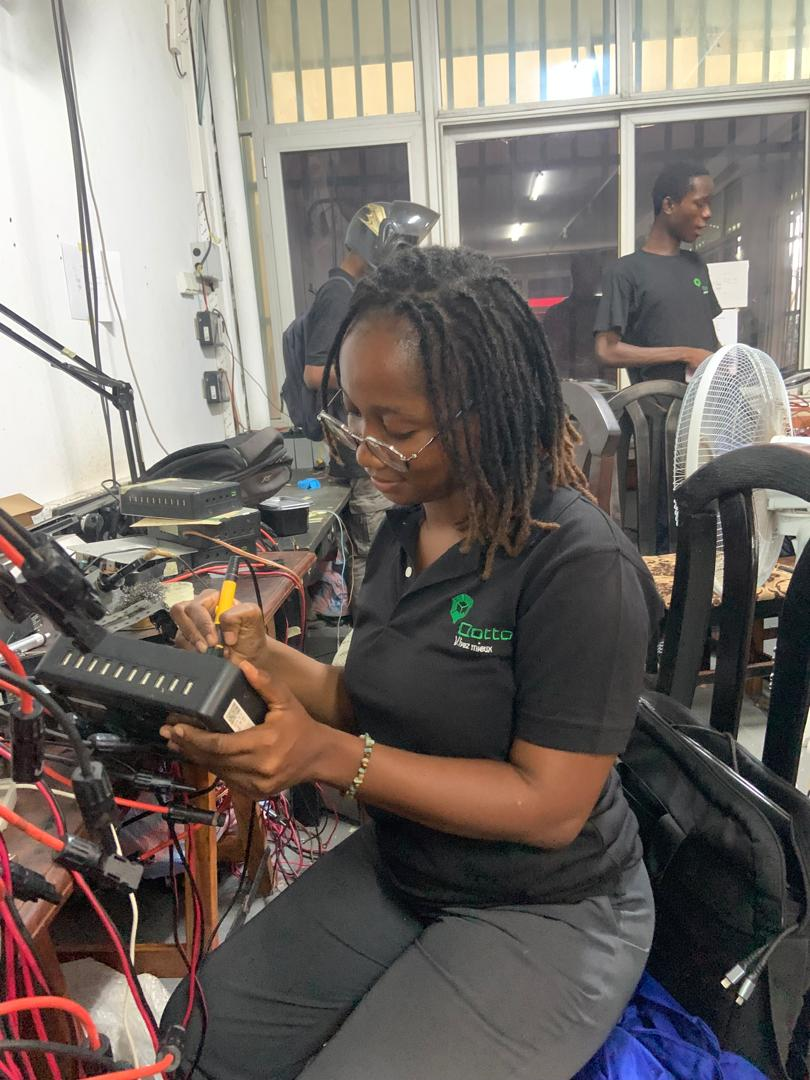
\includegraphics[width=\textwidth]{images/qotto_christelle.jpg}
        \caption{Christelle — diagnostic BMS}
    \end{subfigure}
    \hfill
    \begin{subfigure}[b]{0.47\textwidth}
        \centering
        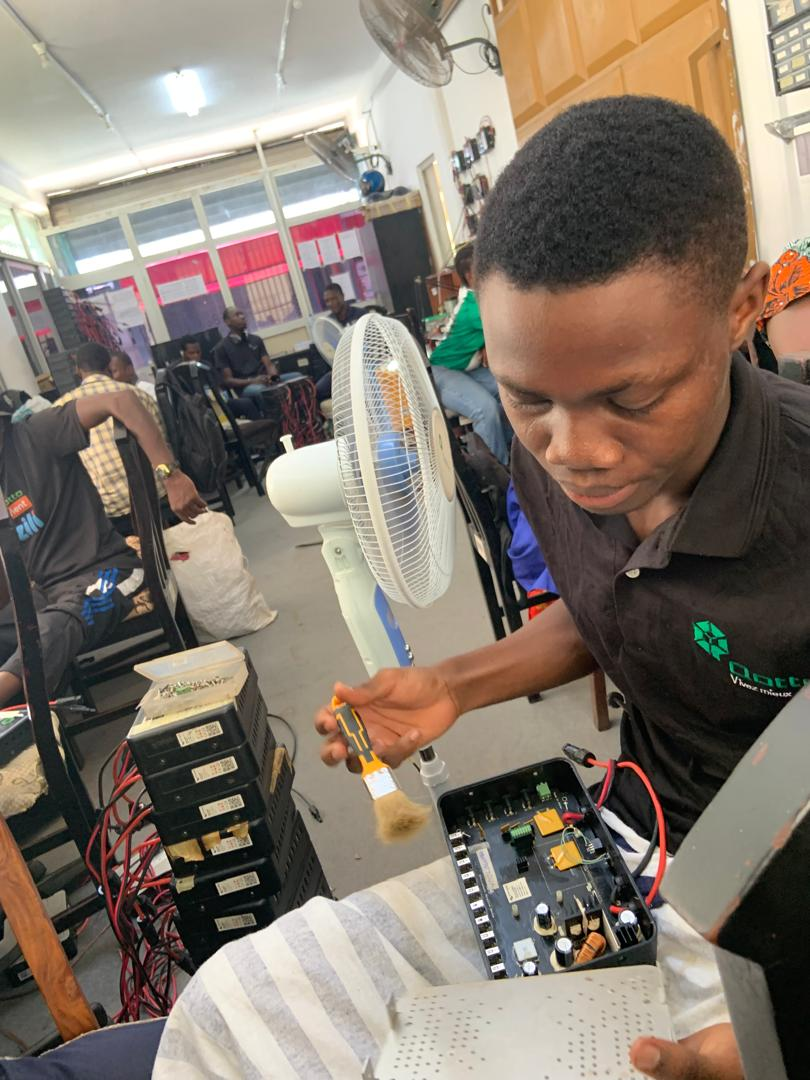
\includegraphics[width=\textwidth]{images/qotto_virgile.jpg}
        \caption{Virgile — reconditionnement}
    \end{subfigure}
    \caption{Les stagiaires en activité au sein de QOTTO Bénin}
    \label{fig:stagiaires_qotto}
\end{figure}
\FloatBarrier

\section{Déroulement des activités}
Afin d'appréhender l'ensemble des métiers de l'entreprise, une rotation hebdomadaire entre les différents postes techniques a été mise en place.

\subsection{Maintenance industrielle des systèmes solaires (BMS/Box)}
Le cœur de notre activité quotidienne a consisté à intervenir sur la chaîne de reconditionnement des BMS et des Box Qotto. Le processus industriel suit un flux rigoureux illustré par la Figure \ref{fig:flux_maintenance}.

\begin{figure}[H]
    \centering
    \begin{tikzpicture}[node distance=1.5cm, every node/.style={fill=white, font=\small}, align=center]
        % Styles
        \tikzstyle{process} = [rectangle, minimum width=5cm, minimum height=0.8cm, text centered, draw=ucaoBlue, fill=ucaoVeryLightBlue, line width=1pt, rounded corners]
        \tikzstyle{arrow} = [thick,->,>=stealth, ucaoBlue]
        
        % Nodes
        \node (start) [process] {1. Entrepôt : Réception, Acquisition et Répartition};
        \node (labo) [process, below of=start] {2. Laboratoire : Calibrage et Mises à jour};
        \node (test1) [process, below of=labo] {3. Poste Test Niveau 1 : Clavier, Ports, Activation};
        \node (rep1) [process, below of=test1] {4. Poste Réparation Niveau 1 (Clavier, Écran, Micro-contrôleur)};
        \node (rep2) [process, below of=rep1] {5. Poste Réparation Niveau 2 (Résistances, Ports)};
        \node (nonreg) [process, below of=rep2] {6. Poste Test de Non-régression};
        \node (recond) [process, below of=nonreg] {7. Reconditionnement : Nettoyage et Fermeture};

        % Arrows
        \draw [arrow] (start) -- (labo);
        \draw [arrow] (labo) -- (test1);
        \draw [arrow] (test1) -- (rep1);
        \draw [arrow] (rep1) -- (rep2);
        \draw [arrow] (rep2) -- (nonreg);
        \draw [arrow] (nonreg) -- (recond);
    \end{tikzpicture}
    \caption{Chaîne opérationnelle de reconditionnement des équipements QOTTO}
    \label{fig:flux_maintenance}
\end{figure}

L'organisation repose sur une rotation hebdomadaire des stagiaires entre les différents postes clés :
\begin{itemize}
    \item \textbf{Flux initial (Entrepôt) :} Après la réception, chaque BMS subit une phase d'acquisition de données. Les équipements sont ensuite répartis par catégories de pannes (problème panneau, clavier déprogrammé, etc.) avant leur transfert au laboratoire.
    \item \textbf{Traitement au Laboratoire :} Cette étape est dédiée au calibrage des BMS et à la mise à jour logicielle des systèmes.
    \item \textbf{Poste Test de Niveau 1 :} On y vérifie l'intégrité des claviers et des ports, suivie de la procédure d'activation. En cas de défaut, l'unité est orientée vers les postes de réparation.
    \item \textbf{Ateliers de Réparation (Niveau 1 et 2) :} Le niveau 1 traite les pannes d'interface (micro, écran, clavier). Le niveau 2 gère les problèmes de ports USB/DC et les alertes critiques nécessitant le remplacement de résistances ou de composants de puissance.
    \item \textbf{Contrôle et Clôture :} Chaque unité réparée subit un test de non-régression au "Poste 2" avant de rejoindre le reconditionnement pour le nettoyage final et la fermeture.
\end{itemize}

\subsection{Recherche et Développement (RD)}
Nous avons également collaboré avec le pôle RD sur les aspects liés à l'ingénierie système :
\begin{itemize}
    \item \textbf{Dimensionnement énergétique :} Apprentissage des méthodes de calcul (sous Google Sheets) pour la constitution d'offres de kits solaires adaptés aux besoins des clients (évaluation de la consommation pour des solutions allant de 3~kW à 5~kW).
    \item \textbf{Validation technologique :} Test de nouveaux kits et solutions innovantes avant leur déploiement massif sur le terrain béninois.
\end{itemize}

\subsection{Application des compétences au projet SMART-SOJA}
Le projet SMART-SOJA constitue la synthèse opérationnelle de notre stage, résultant d'une convergence de compétences acquises au sein de l'écosystème QOTTO. Le diagnostic électronique quotidien sur les BMS a directement renforcé notre capacité à concevoir et déboguer le circuit imprimé du prototype. L'expertise en dimensionnement énergétique obtenue au pôle RD a été transposée pour dimensionner l'alimentation photovoltaïque autonome du projet (panneau 50~W, batterie 12~V/20~Ah, régulateur MPPT). Enfin, l'utilisation des outils de laboratoire (station de soudure, matériel de test) a permis une réalisation physique aux standards professionnels. Cette synergie a permis d'ancrer notre travail académique dans une réalité industrielle concrète.

\section{Bilan du stage et compétences acquises}
Ce stage a permis de développer un ensemble de compétences techniques directement mobilisées dans la réalisation du projet SMART-SOJA :
\begin{itemize}
    \item \textbf{Diagnostic et réparation électronique :} Intervention sur les BMS et Box Qotto (Niveau 1 et 2), compétence réinvestie dans la conception et le débogage du PCB SMART-SOJA.
    \item \textbf{Dimensionnement énergétique :} Calcul de systèmes solaires de 3 à 5~kW, compétence appliquée au dimensionnement de l'alimentation photovoltaïque autonome du prototype.
    \item \textbf{Programmation embarquée :} Mise à jour logicielle et calibrage des systèmes Qotto, compétence transférée au développement du firmware FreeRTOS de l'ESP32.
    \item \textbf{Travail en équipe et documentation :} Suivi de la chaîne de maintenance, rédaction de rapports d'intervention, compétences mises à profit pour la documentation technique du projet.
\end{itemize}

\section{Difficultés rencontrées}
Le déroulement du stage a été marqué par plusieurs contraintes techniques et logistiques :
\begin{itemize}
    \item \textbf{Approvisionnement en composants :} Délais importants pour l'obtention de certains composants électroniques (capteurs, MOSFETs de puissance), accentués par des contraintes budgétaires.
    \item \textbf{Conception mécanique :} Complexité de la modélisation 3D complète du châssis modulaire sous SolidWorks, nécessitant plusieurs itérations.
    \item \textbf{Calibration des capteurs :} Ajustement des sondes d'humidité capacitives pour une mesure fiable sur les grains de soja, en l'absence d'hygromètre de référence certifié au laboratoire.
    \item \textbf{Intégration mécatronique :} Coordination entre les sous-systèmes mécaniques, électroniques et logiciels lors de l'assemblage final du prototype.
\end{itemize}

\section*{Synthèse et transition}
Ce chapitre a présenté le cadre institutionnel du stage effectué au sein de QOTTO Bénin, ainsi que les missions, les activités et les compétences techniques mobilisées durant cette immersion professionnelle. L'expérience acquise en diagnostic électronique, en dimensionnement énergétique et en programmation embarquée au sein de l'entreprise a directement nourri la conception du prototype SMART-SOJA, tandis que les difficultés rencontrées sur le terrain ont orienté certains choix techniques retenus par la suite. Fort de ce cadre pratique et des compétences ainsi consolidées, le chapitre suivant présente l'étude complète de la solution proposée, depuis l'analyse du contexte de la filière soja jusqu'à la réalisation du prototype.
              % Chap 1 : Déroulement du stage
% ================== CHAPITRE 2 : ÉTUDE DE LA SOLUTION PROPOSÉE ==================
% Fusion des anciens chapitres 2 (Contexte), 3 (Matériels/Méthodes) et 4 (Conception)
\chapter{Étude de la solution proposée}

Ce chapitre présente l'ensemble de l'étude menée pour la conception du système \textbf{SMART-SOJA}. Il couvre le contexte de la filière soja et les exigences de qualité, l'état de l'art des technologies mobilisées, le cahier des charges, l'architecture fonctionnelle, les choix techniques (mécaniques, électroniques, énergétiques et logiciels), le dimensionnement des principaux éléments ainsi que la réalisation du prototype.

% -------------------------------------------------------
% PARTIE 1 : CONTEXTE ET ÉTAT DE L'ART
% -------------------------------------------------------

% ---- SECTION CONTEXTE ET ÉTAT DE L'ART ----

% -------------------------------------------------------
\section{La filière soja au Bénin (\textit{Glycine max})}
% -------------------------------------------------------

\subsection{Importance agronomique et économique}
Le soja (\textit{Glycine max}) est une légumineuse annuelle de la famille des \textit{Fabaceae}, originaire d'Asie de l'Est \cite{ifdcsoy}. Sa double valeur — nutritionnelle (environ 40~\% de protéines et 20~\% de lipides par masse sèche) et agronomique (fixation de l'azote atmosphérique par symbiose avec \textit{Bradyrhizobium japonicum}) — en fait une culture stratégique mondiale.

\begin{figure}[H]
    \centering
    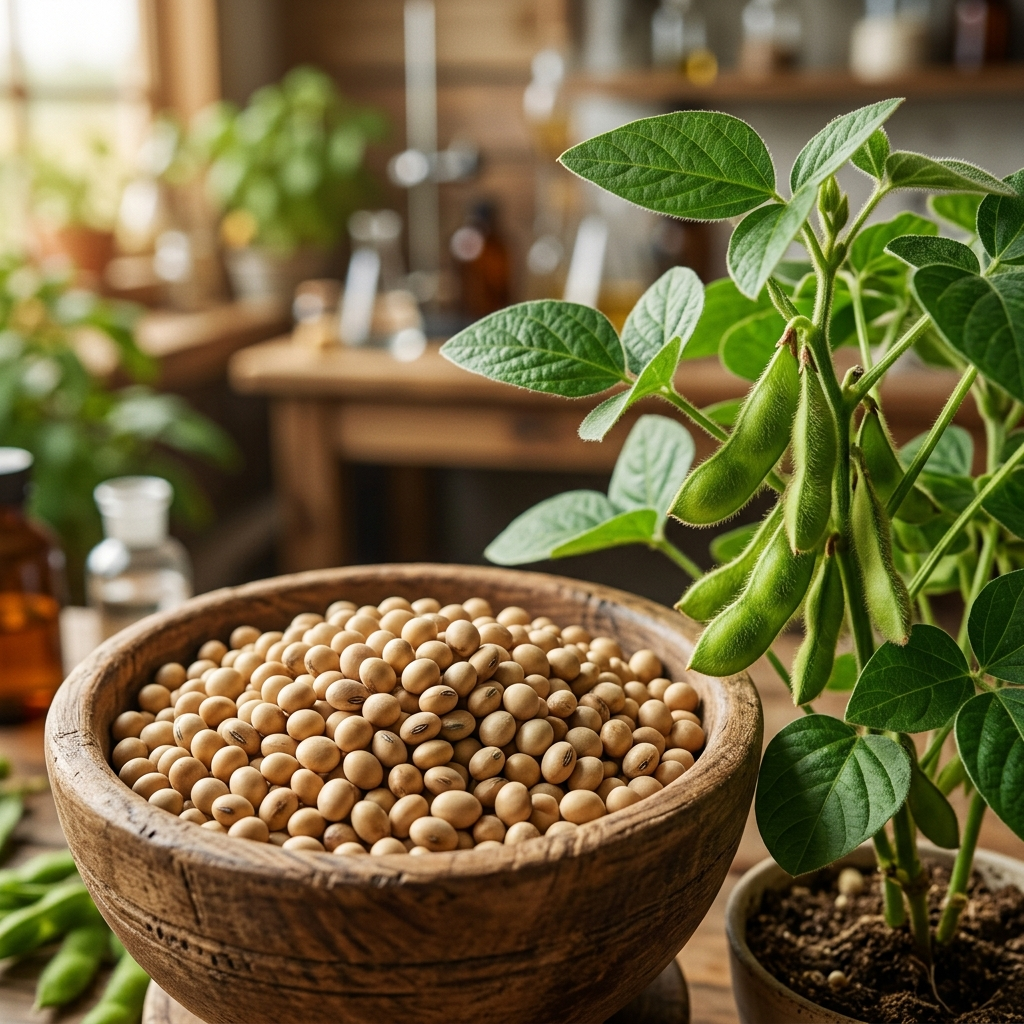
\includegraphics[width=0.45\textwidth]{images/soybean_premium.png}
    \caption{Plante de soja et ses graines (\textit{Glycine max})}
    \label{fig:soybean}
\end{figure}

Au Bénin, la production nationale a connu une progression fulgurante, passant de 157\,620 tonnes en 2015 à plus de 257\,000 tonnes en 2020 \cite{tidjani2023, faostat}, faisant du soja la 4\ieme{} source de devises du pays. Le soja est transformé localement en produits alimentaires (\textit{Wara}, lait, farines infantiles), jouant un rôle vital dans la lutte contre la malnutrition \cite{brab187}. Les variétés les plus répandues appartiennent à la série \textbf{TGX} (TGX 1448-2E, TGX 1910-14F, TGX 1835-10E), sélectionnées pour leur rendement et leur résistance.

\subsection{Enjeux qualitatifs et normes industrielles}
L'émergence de la Zone Industrielle de Glo-Djigbé (GDIZ) constitue le moteur d'une transformation structurelle de la filière \cite{gdiz2023}. Ces unités de trituration modernes imposent des standards stricts, encadrés par l'Agence Nationale de Normalisation à travers la norme \textbf{NB 01.07.004} \cite{anm_soja}. Cette norme, homologuée en 2021, vise à harmoniser les standards de qualité du soja béninois avec les exigences du marché international et des unités de transformations locales :

\begin{enumerate}
    \item \textbf{Taux d'humidité $<$ 12~\% :} Seuil critique pour prévenir les moisissures et assurer la performance des presses à huile.
    \item \textbf{Pureté spécifique $>$ 98~\% :} Absence de débris végétaux, cailloux ou grains brisés.
    \item \textbf{Intégrité du grain :} Limitation des grains cassés pour ne pas altérer la qualité du tourteau.
\end{enumerate}

Or, le diagnostic réalisé par le MAEP et l'UNPS révèle une rupture critique \cite{maep2023, unps2014} : le battage traditionnel et le séchage au sol ne permettent pas d'atteindre ces standards, entraînant des pertes post-récolte de 15~\% à 25~\% et un refoulement régulier des camions aux portes des usines.

\subsection{Étude de l'existant et limites des solutions actuelles}
Plusieurs approches coexistent, mais aucune ne répond simultanément aux contraintes rurales de mobilité, d'autonomie et de traçabilité :

\begin{table}[H]
    \caption{Analyse comparative des solutions de pré-traitement du soja}
    \label{tab:comparaison_soja}
    \centering
    \small
    \renewcommand{\arraystretch}{1.6}
    \rowcolors{2}{white}{lightGray}
    \begin{tabularx}{\textwidth}{|L|C|C|C|}
        \hline
        \rowcolor{lightGray}
        \textbf{Critères} &
        \textbf{Tri Manuel} &
        \textbf{Unités Importées} &
        \textbf{SMART-SOJA} \\ \hline
        Mobilité & Totale & Moyenne & \textbf{Optimisée} \\ \hline
        Source d'énergie & Humaine & Diesel / Réseau & \textbf{Solaire (Autonome)} \\ \hline
        Contrôle humidité & Aléatoire & Non mesurée & \textbf{Précis (Capteur)} \\ \hline
        Traçabilité Internet des objets & Aucune & Aucune & \textbf{Enregistrement numérique au format JSON} \\ \hline
        Accessibilité financière & Nul & Élevé & \textbf{Abordable / Modulaire} \\ \hline
    \end{tabularx}
\end{table}

La solution \textbf{SMART-SOJA} se positionne ainsi comme une approche innovante adaptée au contexte rural : elle déplace la technologie vers la ressource, en garantissant la conformité du grain avant tout acheminement industriel. 

Comme l'illustre le Tableau~\ref{tab:comparaison_soja}, la solution SMART-SOJA surpasse les alternatives existantes sur plusieurs dimensions clés. Contrairement au tri manuel qui reste extrêmement fastidieux, lent et incapable de quantifier scientifiquement le taux d'humidité, notre prototype intègre une mesure électronique précise et reproductible par double sonde capacitive. Par ailleurs, par rapport aux unités de traitement industrielles importées qui exigent un raccordement au réseau triphasé ou l'usage de générateurs diesel polluants et coûteux, SMART-SOJA garantit une autonomie énergétique totale en zone rurale grâce à son alimentation photovoltaïque 12~V. Enfin, sa capacité unique de traçabilité numérique et de communication IoT (génération de payloads JSON via le protocole MQTT) sécurise la chaîne d'approvisionnement en fournissant aux usines de la GDIZ un historique de qualité infalsifiable pour chaque lot avant son transport, réduisant à néant le risque de refoulement aux portes des usines.

% -------------------------------------------------------
\section{Technologies de tri et de nettoyage des grains}
% -------------------------------------------------------

\subsection{Principes physiques de séparation}
La littérature distingue trois principes fondamentaux pour séparer les grains de leurs impuretés \cite{fellows2009, brennan2006} :

\begin{figure}[H]
    \centering
    \begin{subfigure}[b]{0.32\textwidth}
        \centering
        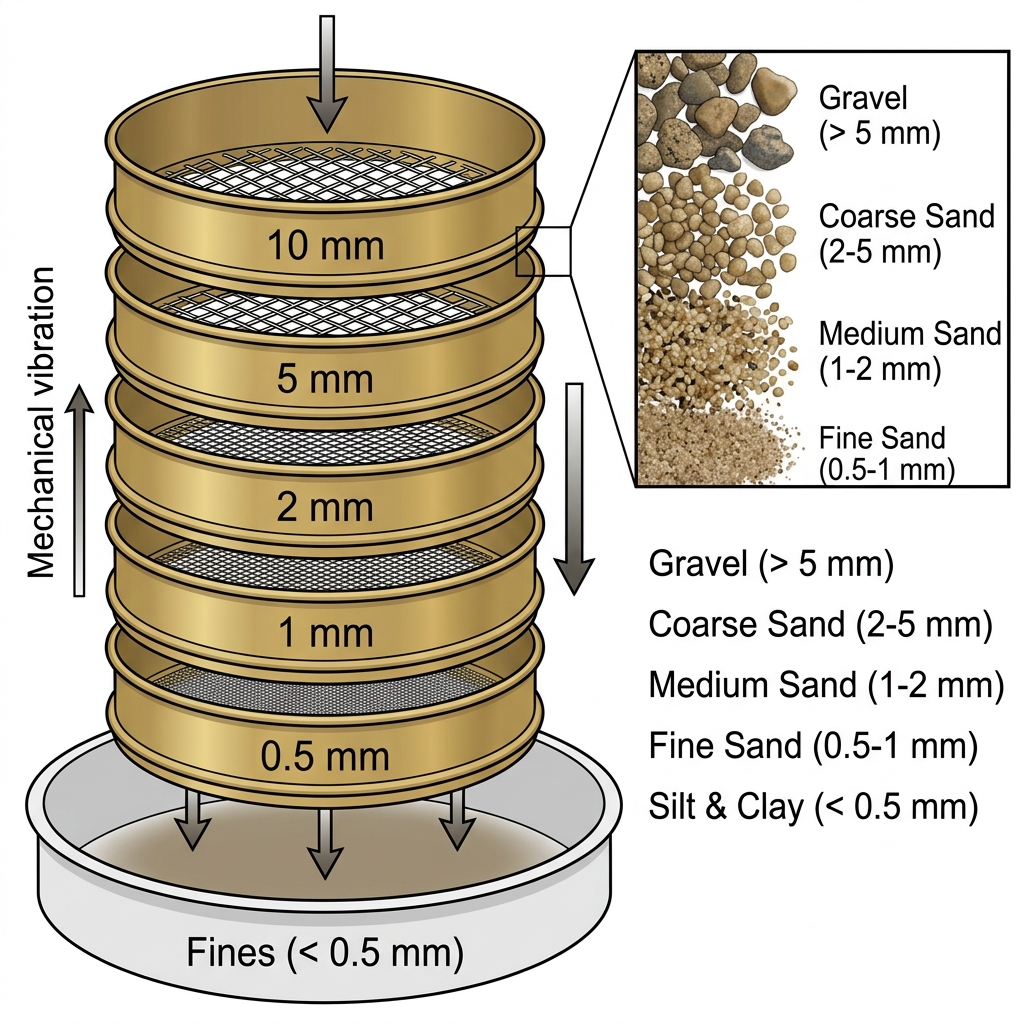
\includegraphics[width=\textwidth]{images/granulometrie.png}
        \caption{Séparation granulométrique}
    \end{subfigure}
    \hfill
    \begin{subfigure}[b]{0.32\textwidth}
        \centering
        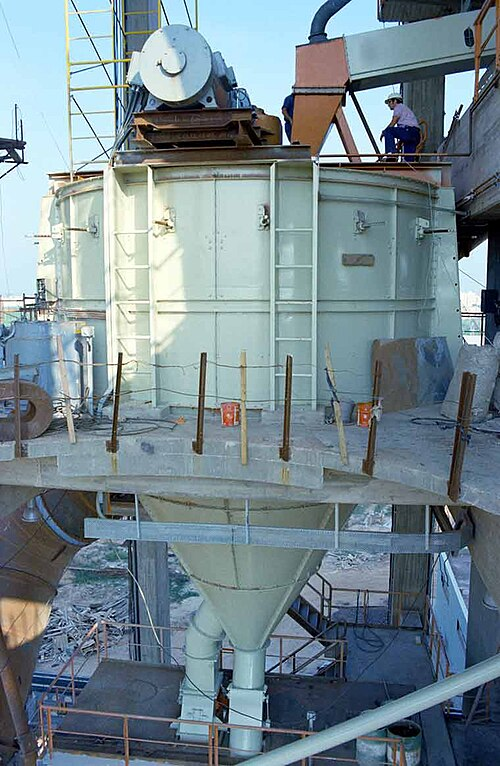
\includegraphics[width=\textwidth, height=4.5cm, keepaspectratio]{images/Zoubov-Sturtevant-whirlwind-centrifugal-Air-classifier-air-separator.jpg}
        \caption{Séparation aéraulique}
    \end{subfigure}
    \hfill
    \begin{subfigure}[b]{0.32\textwidth}
        \centering
        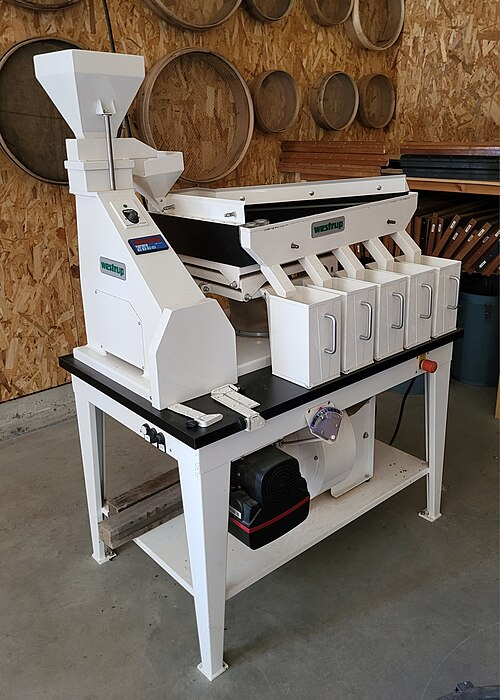
\includegraphics[width=\textwidth, height=4.5cm, keepaspectratio]{images/Table_densimétrique12.jpg}
        \caption{Séparation densimétrique}
    \end{subfigure}
    \caption{Principes physiques de triage des grains}
    \label{fig:tri_physique}
\end{figure}

\begin{itemize}
    \item \textbf{Séparation granulométrique :} Tamis vibrants ou rotatifs classant les grains selon leur taille et leur épaisseur (principe retenu pour le Bloc 2 de SMART-SOJA).
    \item \textbf{Séparation aéraulique :} Flux d'air vertical emportant les impuretés légères (poussières, gousses vides) tout en conservant les grains lourds.
    \item \textbf{Séparation densimétrique :} Table densimétrique exploitant un lit fluidisé pour trier des éléments de même taille mais de densités différentes.
\end{itemize}

\subsection{État de l'art industriel}
Au niveau industriel, les trieurs optiques représentent la solution la plus avancée : ils utilisent des caméras haute résolution et des algorithmes de traitement d'image pour éjecter les grains défectueux par jets d'air comprimé \cite{mahajan2015}. Bien que performants, leur coût élevé et leurs besoins énergétiques importants les rendent inaccessibles aux petits producteurs ruraux, justifiant une approche mécatronique plus abordable pour SMART-SOJA.

\begin{figure}[H]
    \centering
    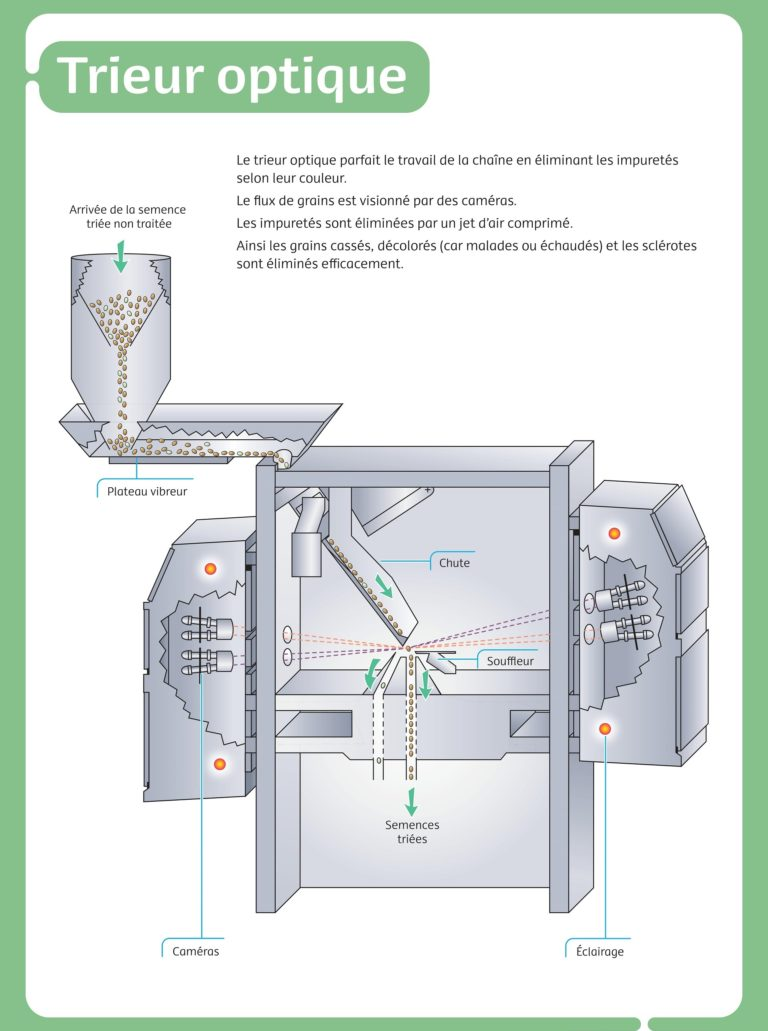
\includegraphics[height=6cm, keepaspectratio]{images/semae-pedagogie-station-semences-trieur-optique-768x1031.jpg}
    \caption{Exemple de trieur optique industriel haute résolution (Source : SEMAE Pédagogie)}
    \label{fig:trieur_optique}
\end{figure}

\FloatBarrier

% -------------------------------------------------------
\section{L'Internet des objets dans le secteur agricole (Agriculture 4.0)}
% -------------------------------------------------------

\subsection{Réseaux de capteurs sans fil (WSN) et connectivité LPWAN}
L'intégration de l'Internet des objets en agriculture (\textit{Smart Farming}) transforme la collecte et l'exploitation des données de terrain \cite{tarekegn2020}. Pour les zones rurales, les technologies \textbf{LPWAN} (\textit{Low-Power Wide-Area Network}) sont particulièrement adaptées en raison de leur longue portée et de leur faible consommation énergétique \cite{hanes2017, tzounis2017}.

\begin{figure}[H]
    \centering
    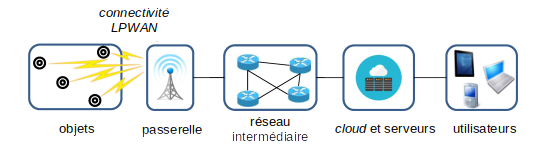
\includegraphics[width=0.65\textwidth]{images/Sensors-LPWAN.png}
    \caption{Architecture de connectivité LPWAN pour capteurs agricoles}
    \label{fig:iot_connectivity}
\end{figure}

Le protocole \textbf{MQTT} (\textit{Message Queuing Telemetry Transport}) constitue le standard de facto de l'Internet des objets industriel léger : son architecture Publication/Abonnement permet une communication robuste sur des réseaux à bande passante limitée et connexion instable, comme les zones rurales du Bénin \cite{mqtt_org, hanes2017}.

\subsection{Traçabilité numérique et Big Data agricole}
La numérisation des données de qualité crée un \textit{passeport numérique} du grain depuis le champ jusqu'à l'usine. Les travaux de recherche montrent que la structuration de ces données en format \textbf{JSON} permet de limiter les fraudes, de garantir les standards qualité de la GDIZ et d'ouvrir la voie à des analyses prédictives (Big Data agricole) pour l'amélioration continue des processus.


\subsection{Autonomie énergétique en milieu rural}
L'électrification rurale étant défaillante dans de nombreuses zones de production, la littérature technique privilégie les systèmes photovoltaïques hybrides avec régulateurs \textbf{MPPT} (\textit{Maximum Power Point Tracking}) pour optimiser l'extraction d'énergie solaire, abondante dans les régions tropicales comme le Bénin.

\FloatBarrier

% -------------------------------------------------------
\section{Cahier des charges fonctionnel}
% -------------------------------------------------------

L'analyse du contexte de la filière soja, des exigences normatives (NB~01.07.004) et des limites des solutions existantes permet de formuler le cahier des charges fonctionnel du système SMART-SOJA. Ce document de référence définit les fonctions que le prototype doit remplir, les critères d'acceptation et les moyens de validation associés. Les fonctions sont classées en \textbf{fonctions principales} (FP), directement liées aux objectifs du système, et en \textbf{fonctions contraintes} (FC), imposées par l'environnement d'utilisation.

\subsection{Fonctions principales}

Le Tableau~\ref{tab:cdc_fp} détaille les sept fonctions principales du système, issues des objectifs spécifiques du mémoire et des exigences de la norme \textbf{NB~01.07.004}.

\begin{table}[H]
    \caption{Cahier des charges fonctionnel — Fonctions principales (FP)}
    \label{tab:cdc_fp}
    \centering
\footnotesize
\renewcommand{\arraystretch}{1.5}
\rowcolors{2}{white}{lightGray}
\begin{tabularx}{\textwidth}{|p{2.3cm}|L|p{2.1cm}|L|L|}
\hline
\rowcolor{lightGray}
\textbf{Fonction} & \textbf{Exigence} & \textbf{Valeur cible} & \textbf{Justification} & \textbf{Moyen de vérification} \\ \hline

\textbf{FP1}\newline Nettoyage &
Séparer les impuretés des grains par tamisage vibrant &
Pureté $>$ 98~\% &
Norme NB~01.07.004, exigence GDIZ &
Pesée différentielle avant/après, inspection visuelle \\ \hline

\textbf{FP2}\newline Mesure humidité &
Mesurer le taux d'humidité en deux points du lot (Soil1/Soil2) &
$\pm\,5$~\% HR, seuil 12~\% &
Norme NB~01.07.004 &
Comparaison avec hygromètre de référence certifié \\ \hline

\textbf{FP3}\newline Séchage actif &
Réduire l'humidité par air chaud et brassage si $H > 12$~\% &
$H \leq 12$~\% en sortie (double validation) &
Prévention moisissures, conformité GDIZ &
Lecture convergente Soil1 ET Soil2 $\leq$ 12~\% \\ \hline

\textbf{FP4}\newline Pesée &
Peser chaque lot traité avec précision &
0--10~kg, $\pm\,0{,}1$~\% &
Certification du poids pour traçabilité &
Étalonnage poids de référence (module HX711) \\ \hline

\textbf{FP5}\newline Traçabilité IoT &
Générer un passeport numérique JSON par lot et le transmettre via MQTT &
Payload JSON complet, publication MQTT &
Transparence et fiabilité de la chaîne d'approvisionnement &
Réception et décodage sur broker HiveMQ \\ \hline

\textbf{FP6}\newline Autonomie &
Fonctionner en autonomie solaire hors réseau électrique &
$\geq$ 3~h/jour, recharge solaire en 5~h &
Zones rurales non électrifiées &
Mesure tension batterie, durée de cycle effective \\ \hline

\textbf{FP7}\newline Mobilité &
Déplacer l'unité vers les sites de collecte &
Châssis sur roulettes, compatible véhicule utilitaire &
Rapprocher la technologie du producteur &
Test de déplacement sur terrain plat et piste \\ \hline

\end{tabularx}
\end{table}

\subsection{Fonctions contraintes}

Le Tableau~\ref{tab:cdc_fc} regroupe les contraintes imposées par l'environnement opérationnel, la sécurité et la maintenabilité du système.

\begin{table}[H]
    \caption{Cahier des charges fonctionnel — Fonctions contraintes (FC)}
    \label{tab:cdc_fc}
    \centering
\footnotesize
\renewcommand{\arraystretch}{1.5}
\rowcolors{2}{white}{lightGray}
\begin{tabularx}{\textwidth}{|p{2.3cm}|L|p{2.1cm}|L|L|}
\hline
\rowcolor{lightGray}
\textbf{Fonction} & \textbf{Exigence} & \textbf{Valeur cible} & \textbf{Justification} & \textbf{Moyen de vérification} \\ \hline

\textbf{FC1}\newline Interface opérateur &
Affichage et contrôle local du cycle &
LCD 16$\times$2, 2 potentiomètres, boutons, LEDs &
Opérateur non expert en milieu rural &
Test d'utilisabilité en conditions réelles \\ \hline

\textbf{FC2}\newline Contrôle temps réel &
Automatisation séquentielle (GRAFCET) avec sécurité prioritaire &
Temps de réponse sécurité $<$ 10~ms &
Sûreté de fonctionnement, arrêt d'urgence &
Test arrêt d'urgence, chronogramme FreeRTOS \\ \hline

\textbf{FC3}\newline Résilience réseau &
Aucune perte de données en l'absence de WiFi &
\textit{Store-and-Forward} sur carte MicroSD &
Couverture WiFi limitée en zone rurale &
Test déconnexion/reconnexion, intégrité données \\ \hline

\textbf{FC4}\newline Maintenabilité &
Accès individuel aux sous-systèmes sans démontage intégral &
4 blocs amovibles, connecteurs rapides &
Maintenance en milieu rural isolé &
Démontage et remontage d'un bloc $<$ 15~min \\ \hline

\textbf{FC5}\newline Robustesse &
Résistance aux vibrations, poussière et chocs de transport &
Châssis acier 40~mm, tamis inox 304, roulettes caoutchouc &
Usage en extérieur, transport sur pistes &
Inspection visuelle après campagne de tests \\ \hline

\textbf{FC6}\newline Coût &
Accessibilité financière du prototype &
Composants standard, disponibles localement &
Cible : coopératives et petits producteurs &
Bilan financier détaillé des composants \\ \hline

\end{tabularx}
\end{table}

Ce cahier des charges constitue le document de référence pour la suite de l'étude. Chaque fonction sera traitée dans les sections suivantes à travers les choix d'architecture, de composants et de dimensionnement du système SMART-SOJA.

% Fin de la section contexte


% -------------------------------------------------------
% PARTIE 2 : MATÉRIELS ET MÉTHODES
% -------------------------------------------------------

% ---- SECTION MATÉRIELS ET MÉTHODES ----

% -------------------------------------------------------
\section{Architecture système globale}
% -------------------------------------------------------
Le système \textbf{SMART-SOJA} repose sur une architecture modulaire et hiérarchisée structurée en trois couches fonctionnelles (Figure \ref{fig:architecture_complete}) :

\begin{figure}[H]
    \centering
    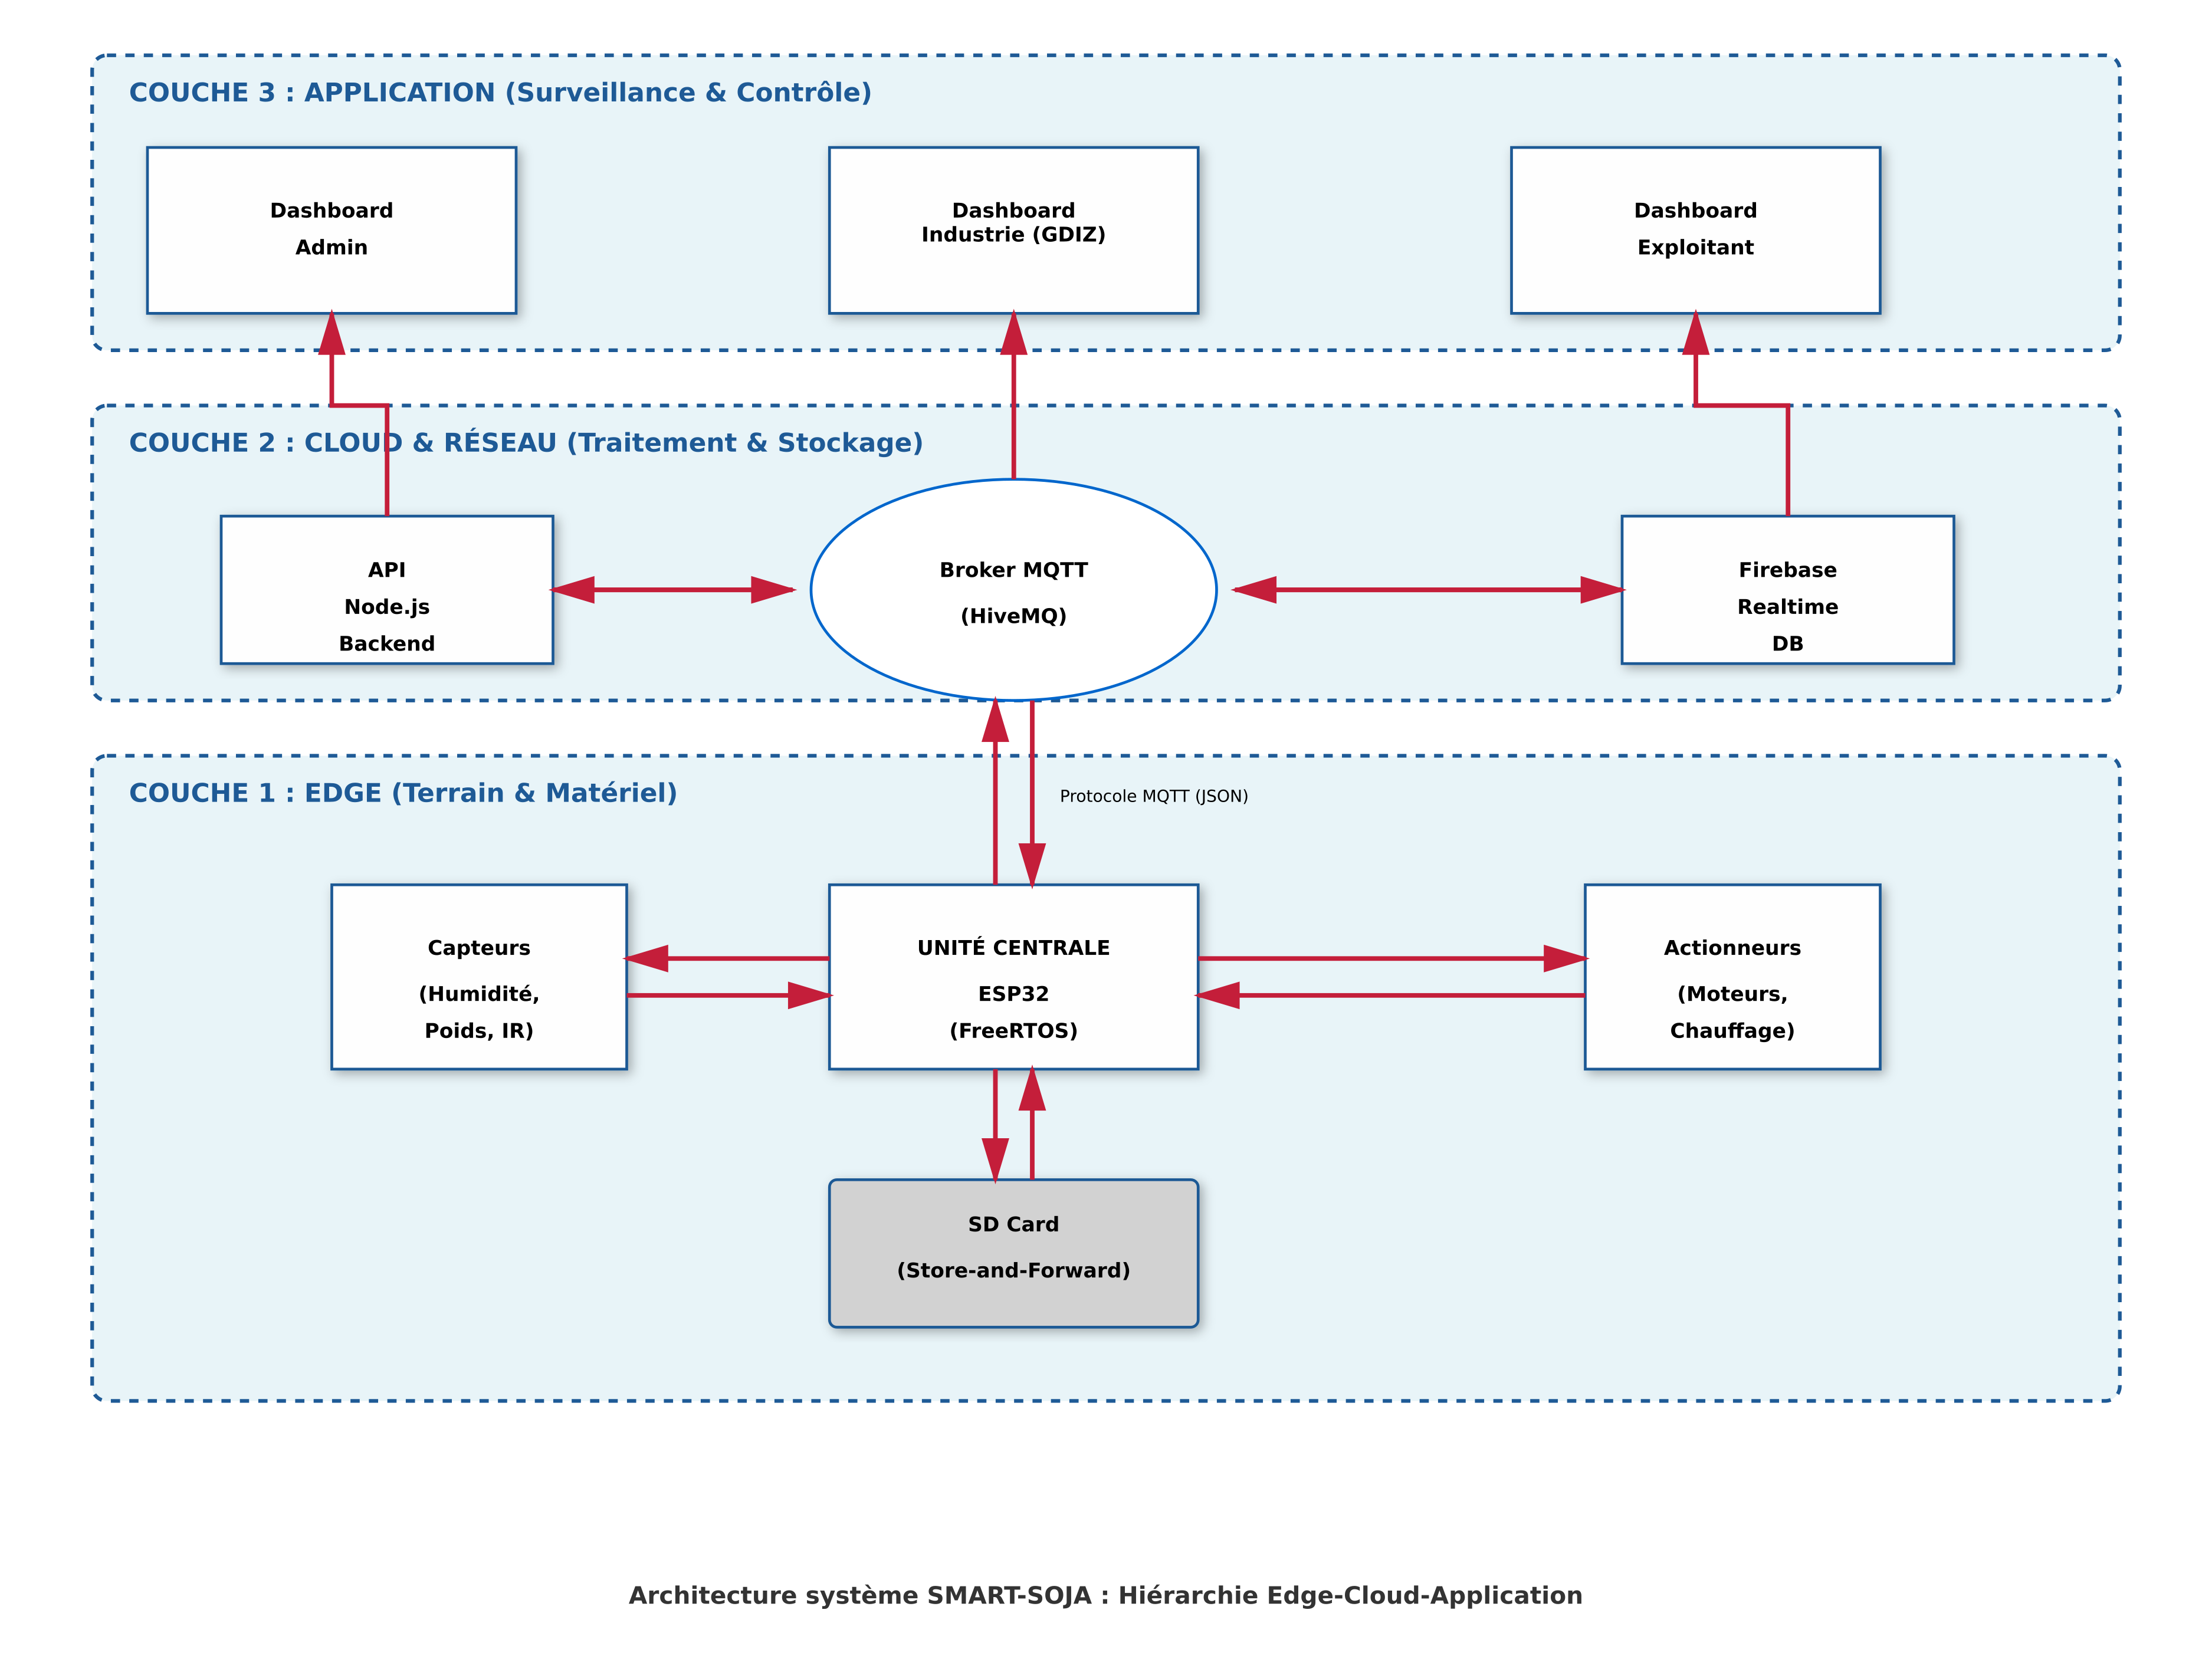
\includegraphics[width=\textwidth]{images/architecture_smart_soja.png}
    \caption{Architecture système SMART-SOJA : Hiérarchie Edge-Cloud-Application}
    \label{fig:architecture_complete}
\end{figure}
\FloatBarrier

\begin{itemize}
    \item \textbf{Couche Edge (Terrain) :} L'ESP32 gère en temps réel l'acquisition des capteurs, le pilotage des actionneurs et la logique de contrôle GRAFCET.
    \item \textbf{Couche Cloud :} Un broker MQTT (HiveMQ) relié à une API Node.js et une base Firebase assure le stockage et le traitement des données de traçabilité.
    \item \textbf{Couche Application :} Des tableaux de bord web (rôles Admin, Industrie, Exploitant) permettent le suivi à distance de chaque lot traité.
\end{itemize}

Cette architecture (Figure \ref{fig:architecture_complete}) garantit un fonctionnement autonome complet en mode déconnecté (\textit{Store-and-Forward} sur carte SD), tout en s'intégrant nativement dans une infrastructure Cloud de type Industrie 4.0. Elle permet une résilience face aux pannes de réseau fréquentes en milieu rural tout en assurant une visibilité globale pour les unités de transformation.

% -------------------------------------------------------
\section{Sous-système électronique et informatique}
% -------------------------------------------------------

\subsection{Unité de traitement : l'ESP32-WROOM-32}

Le microcontrôleur \textbf{ESP32-WROOM-32} (Figure \ref{fig:esp32_presentation}) constitue le cœur décisionnel du système \cite{esp32_datasheet}. Ses spécifications techniques sont résumées dans le Tableau \ref{tab:specs_esp32}.

\begin{table}[H]
    \caption{Spécifications techniques du microcontrôleur ESP32-WROOM-32}
    \label{tab:specs_esp32}
    \centering
    \small
    \renewcommand{\arraystretch}{1.4}
    \rowcolors{2}{white}{lightGray}
    \begin{tabularx}{\textwidth}{|L|>{\bfseries}L|}
        \hline
        \rowcolor{lightGray}
        \textbf{Caractéristique} & \textbf{Spécification} \\ \hline
        Microcontrôleur & Tensilica LX6 double cœur 240 MHz \\ \hline
        Alimentation & 5~V DC (microUSB) / 3,3~V DC (E/S) \\ \hline
        Consommation veille & 5~\textmu A (Ultra-low power) \\ \hline
        Mémoire & 520 Ko SRAM / 4 Mo Flash \\ \hline
        Connectivité & Wi-Fi 802.11 b/g/n + Bluetooth 4.2 \\ \hline
        GPIO & 30 broches (3x UART, 2x I2C, 3x SPI, 12x ADC, 2x DAC) \\ \hline
        Dimensions & 55 × 28 × 8 mm / 11 g \\ \hline
    \end{tabularx}
\end{table}

\begin{figure}[H]
    \centering
    \begin{subfigure}[b]{0.45\textwidth}
        \centering
        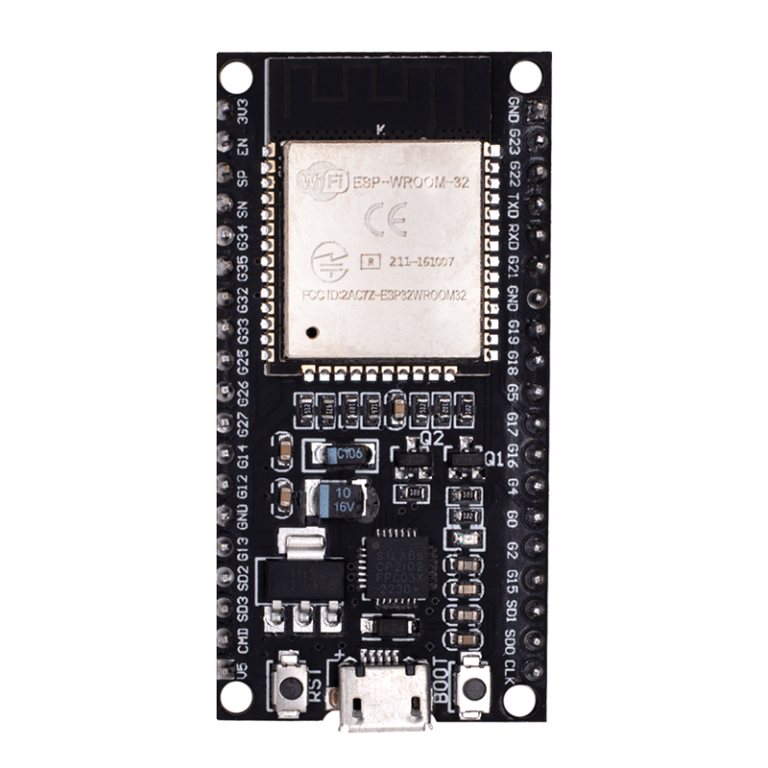
\includegraphics[width=\textwidth]{images/image_esp32.png}
        \caption{Module ESP32-WROOM-32}
    \end{subfigure}
    \hfill
    \begin{subfigure}[b]{0.45\textwidth}
        \centering
        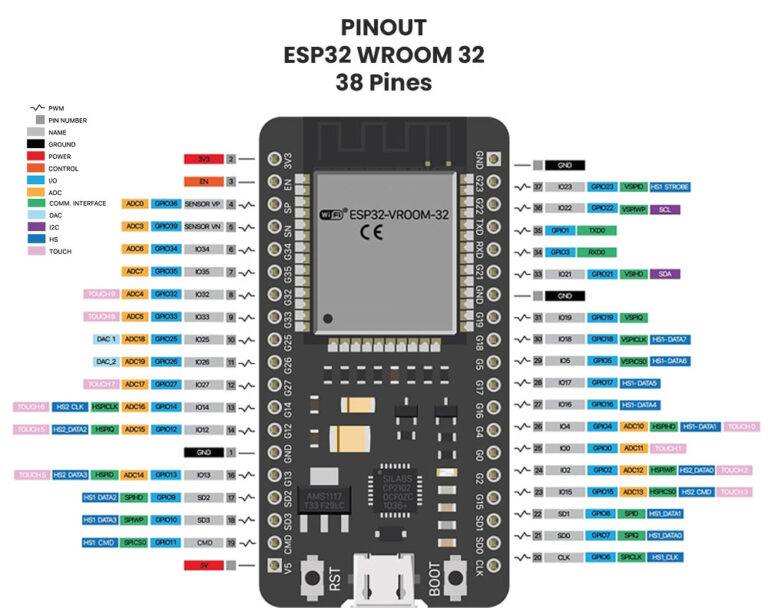
\includegraphics[width=\textwidth]{images/pinout_esp32.jpg}
        \caption{Brochage (Pinout)}
    \end{subfigure}
    \caption{Présentation du microcontrôleur ESP32}
    \label{fig:esp32_presentation}
\end{figure}
\FloatBarrier

\textbf{Justification du choix :} L'architecture Dual-Core permet de dédier un cœur au contrôle-commande temps réel (capteurs, actionneurs PWM) et l'autre à la communication Internet des objets (MQTT/WiFi), garantissant un déterminisme critique. La consommation de 5~\textmu A en veille optimise l'autonomie solaire, et les 30 GPIO offrent la flexibilité nécessaire pour tous les bus I2C, SPI et interfaces ADC du système.

\subsection{Chaîne d'acquisition : les capteurs}

Quatre capteurs stratégiques (Figure \ref{fig:capteurs_systeme}) assurent le suivi de la qualité et le déclenchement automatique des actions du GRAFCET (Tableau \ref{tab:specs_capteurs}).

\begin{table}[H]
    \caption{Spécifications détaillées de la chaîne d'acquisition}
    \label{tab:specs_capteurs}
    \centering
    \small
    \renewcommand{\arraystretch}{1.5}
    \rowcolors{2}{white}{lightGray}
    \begin{tabularx}{\textwidth}{|L|C|C|L|L|}
        \hline
        \rowcolor{lightGray}
        \textbf{Capteur} & \textbf{Plage / Précision} & \textbf{Calibration} & \textbf{Rôle} & \textbf{Limites} \\ \hline
        DHT22 & 0-100\% RH / ±2\% & Usine (1-Wire) & Humidité/Temp. ambiante & Temps réponse 2s \\ \hline
        Sonde Capacitive & 0-100\% (HR equiv.) / ±5\% & In-situ (soja sec/humide) & Humidité grains (Soil1, Soil2) & Dérive thermique \\ \hline
        IR Réflectif & 2-30 cm / Binaire & Trimpot manuel & Présence trémie/sac & Lumière ambiante \\ \hline
        Cellule de charge & 0-10 kg / ±0,1\% & Poids étalon (HX711) & Pesée finale du lot & Vibrations mécaniques \\ \hline
    \end{tabularx}
\end{table}

\begin{figure}[H]
    \centering
    \begin{subfigure}[b]{0.22\textwidth}
        \centering
        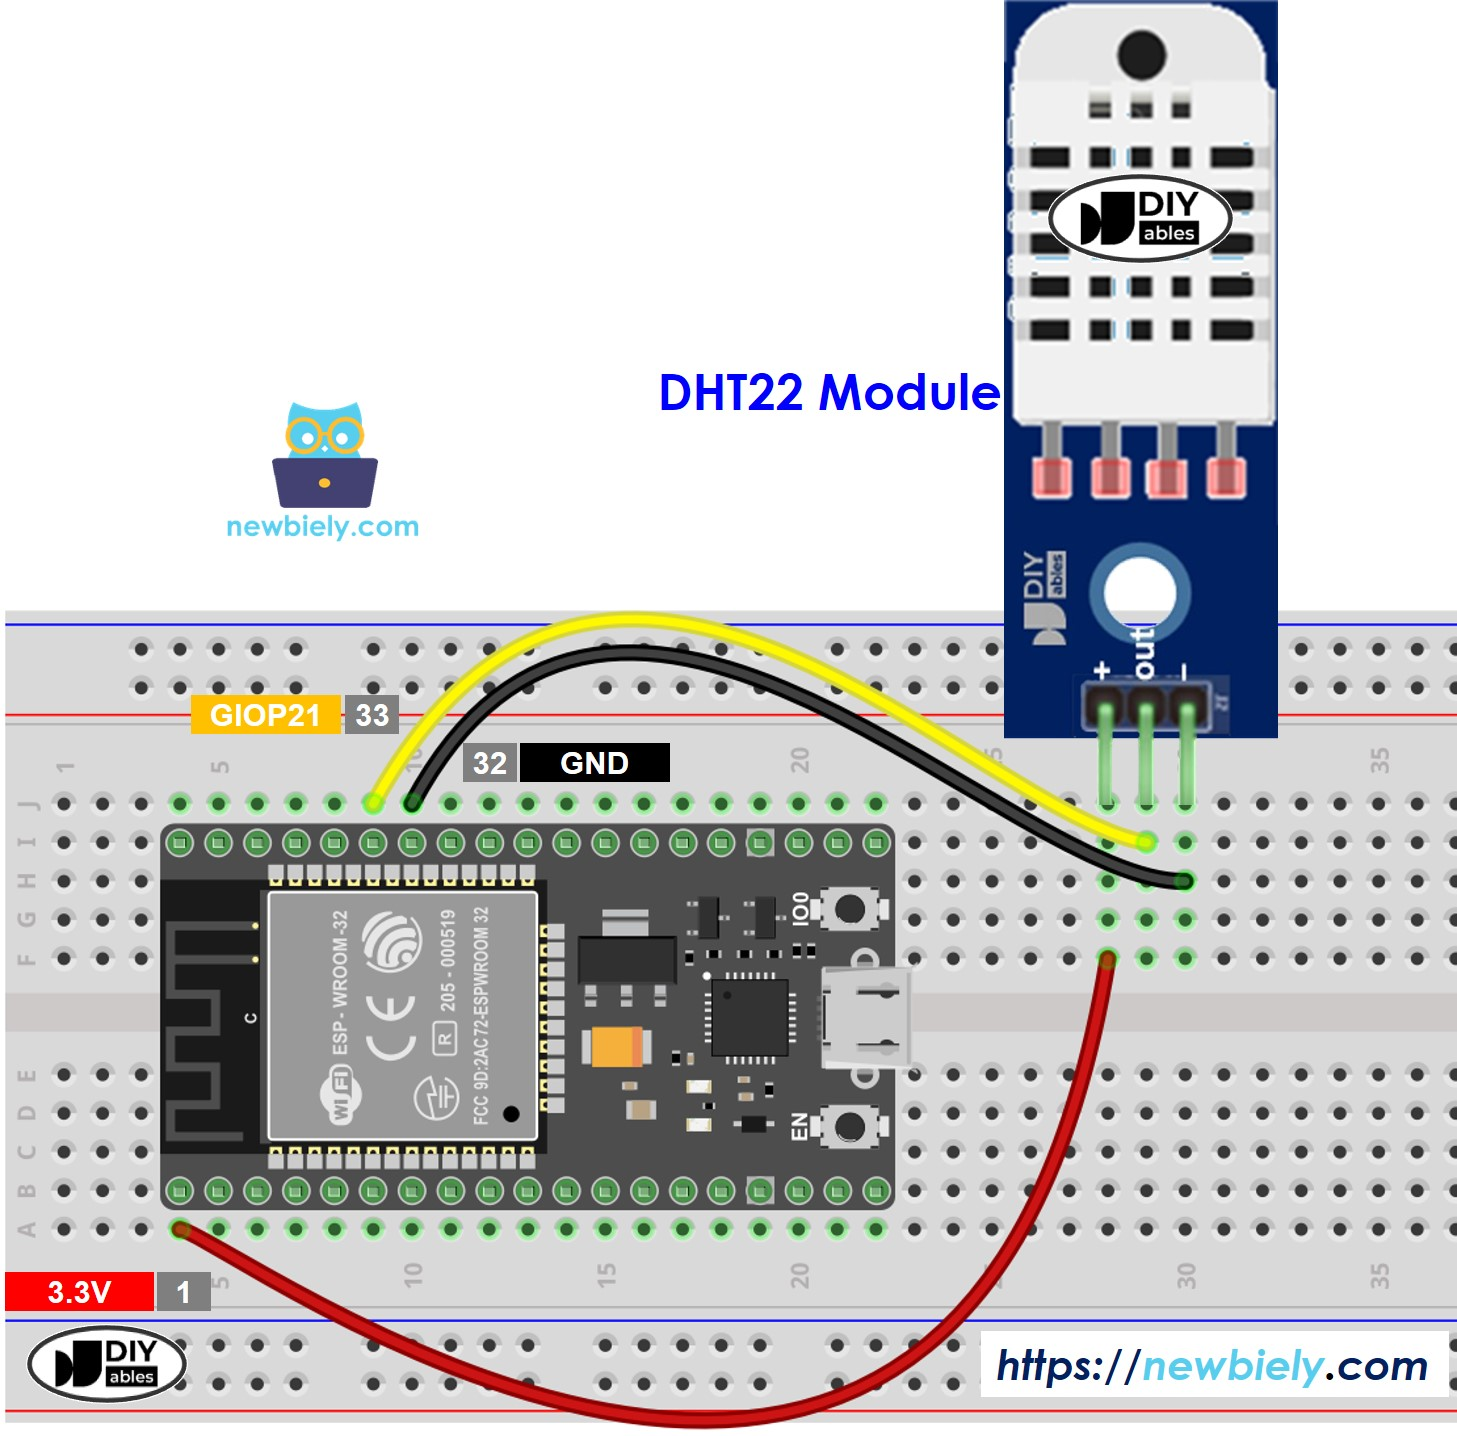
\includegraphics[width=\textwidth]{images/esp32-dht22-module-broche3.jpg}
        \caption{DHT22}
    \end{subfigure}
    \hfill
    \begin{subfigure}[b]{0.22\textwidth}
        \centering
        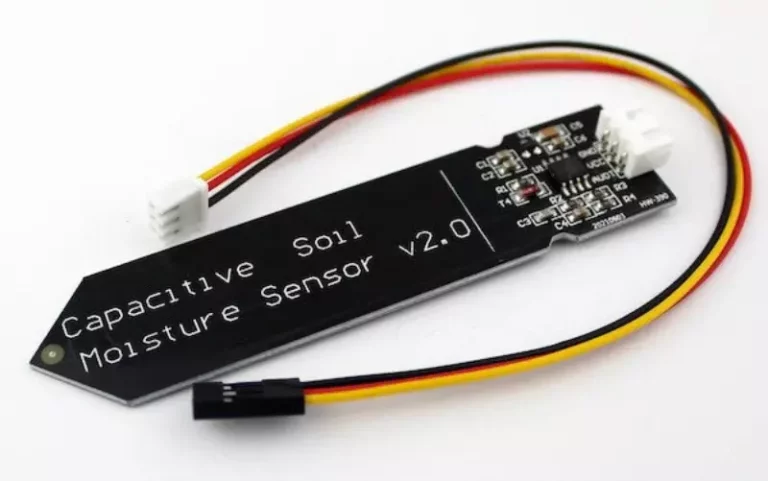
\includegraphics[width=\textwidth]{images/Capacitive-Soil-Moisture-Sensor-768x481.png}
        \caption{Sonde capacitive}
    \end{subfigure}
    \hfill
    \begin{subfigure}[b]{0.22\textwidth}
        \centering
        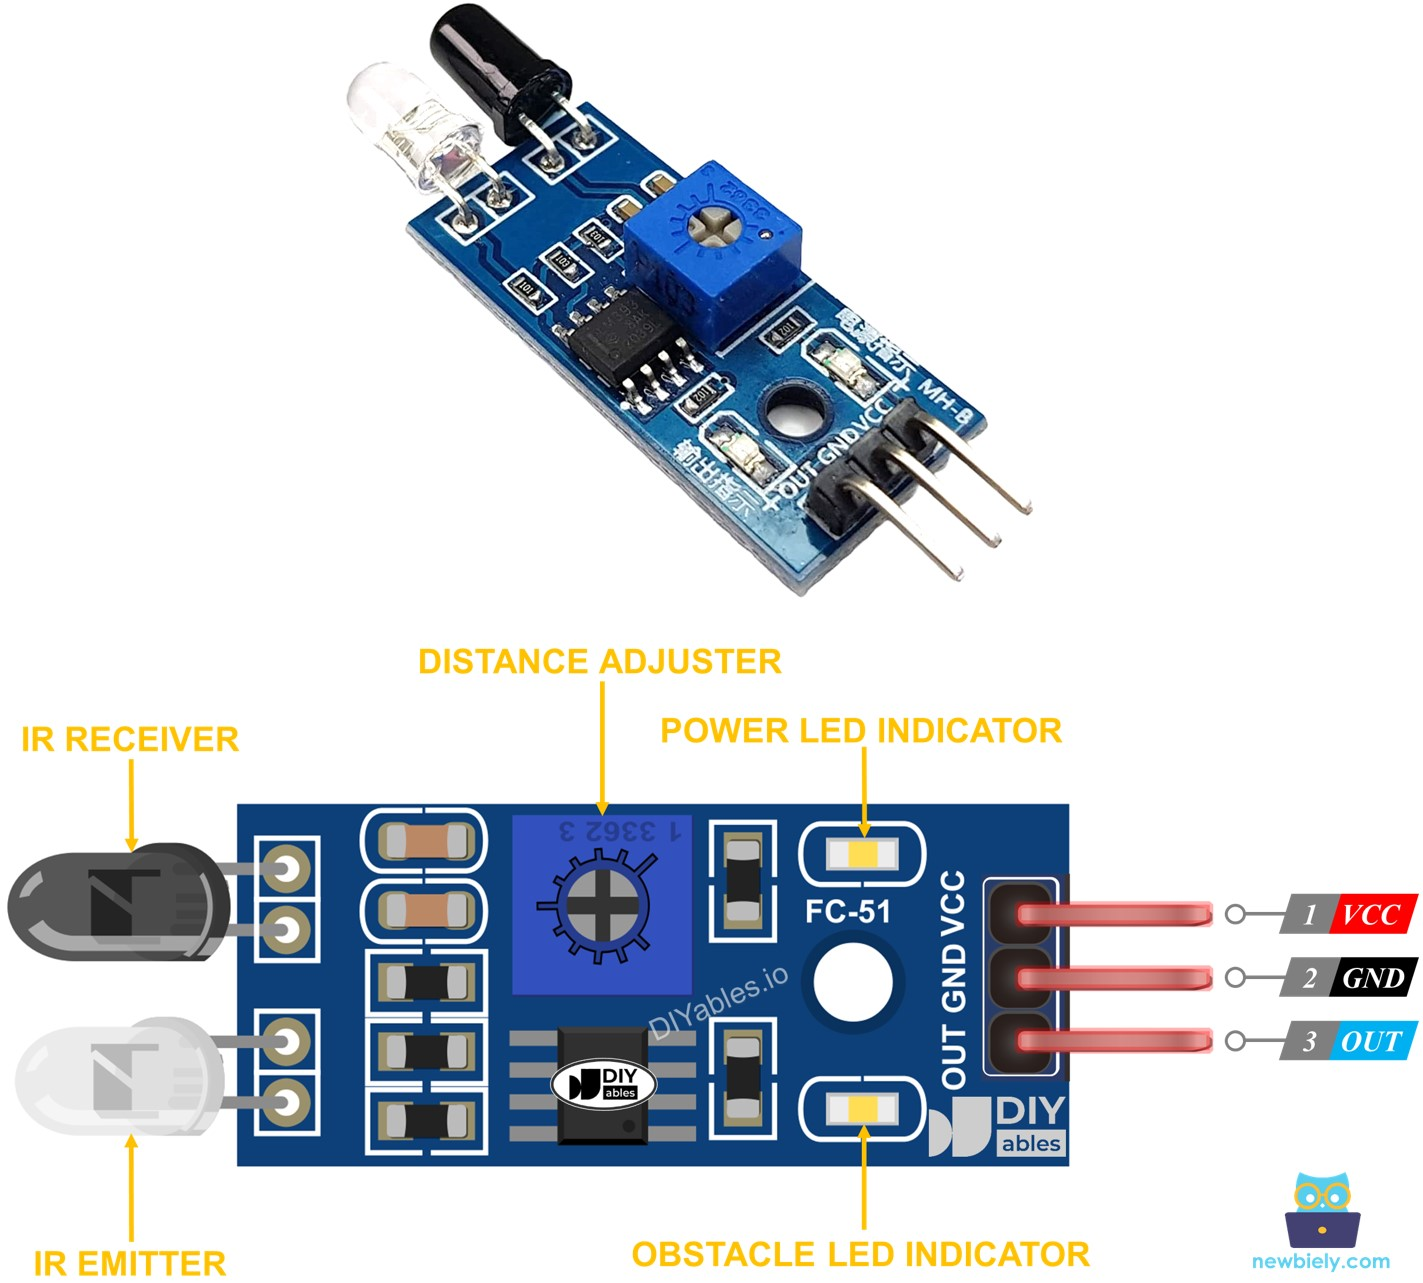
\includegraphics[width=\textwidth]{images/IR-avoidance-sensor-pinout.jpg}
        \caption{Capteur IR}
    \end{subfigure}
    \hfill
    \begin{subfigure}[b]{0.22\textwidth}
        \centering
        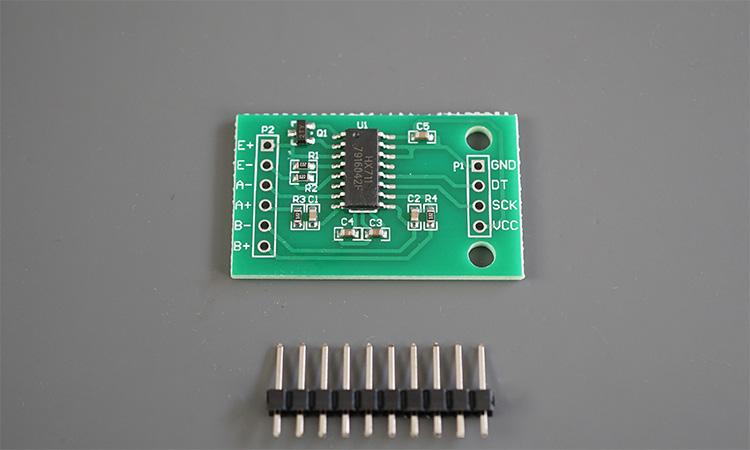
\includegraphics[width=\textwidth]{images/hx711-amplifier.jpg}
        \caption{Module HX711}
    \end{subfigure}
    \caption{Capteurs intégrés au système SMART-SOJA}
    \label{fig:capteurs_systeme}
\end{figure}
L'intégration de cette chaîne d'acquisition (Figure \ref{fig:capteurs_systeme}) permet de couvrir l'intégralité des besoins de suivi : l'humidité ambiante influe sur la cinétique de séchage, les sondes capacitives valident la qualité intrinsèque, l'infrarouge gère l'automatisation du flux et la cellule de charge certifie le poids final.

La \textbf{sonde d'humidité capacitive} mérite une attention particulière : elle mesure la constante diélectrique du milieu (eau $\approx$ 80 vs. grain sec $\approx$ 3--5), ce qui la rend insensible à la corrosion — avantage décisif pour un usage en contact direct avec les grains de soja. Deux sondes (Soil1 et Soil2) sont positionnées respectivement en haut et en bas de la zone de séchage, permettant un calcul d'humidité moyenne en deux points.

\textbf{Calibration in-situ :} La sonde capacitive délivre une tension analogique lue par le convertisseur ADC 12 bits de l'ESP32 (plage 0--4095). Une calibration en deux points est réalisée avant chaque campagne d'essai :
\begin{enumerate}
    \item \textbf{Point sec} ($H \approx 8~\%$) : un échantillon de soja séché à l'étuve est placé autour de la sonde ; la valeur ADC correspondante est enregistrée comme borne haute (soja conforme).
    \item \textbf{Point humide} ($H \approx 20~\%$) : un échantillon saturé en humidité sert de borne basse (soja non conforme).
\end{enumerate}
Une interpolation linéaire entre ces deux bornes permet de convertir toute lecture ADC intermédiaire en un taux d'humidité exprimé en pourcentage. Cette méthode simple mais robuste est validée par comparaison avec les mesures de l'hygromètre de référence Testo 608-H2, avec un écart maximal observé de $\pm 5~\%$ conformément à la spécification du capteur (Tableau~\ref{tab:specs_capteurs}).

\subsection{Chaîne d'action : actionneurs et interface de puissance}

Le pilotage des charges électromécaniques (12~V, forts courants) depuis un microcontrôleur 3,3~V nécessite des interfaces de puissance adaptées (Figure \ref{fig:actionneurs_systeme}). Le Tableau \ref{tab:specs_actionneurs} récapitule les actionneurs du système.

\begin{table}[H]
    \caption{Spécifications détaillées de la chaîne d'action}
    \label{tab:specs_actionneurs}
    \centering
    \small
    \renewcommand{\arraystretch}{1.5}
    \rowcolors{2}{white}{lightGray}
    \begin{tabularx}{\textwidth}{|L|C|L|L|}
        \hline
        \rowcolor{lightGray}
        \textbf{Actionneur} & \textbf{Puissance / Courant} & \textbf{Critère de dimensionnement} & \textbf{Protections} \\ \hline
        Moteurs JGA25 & 3~W / 0,5~A (max 1,2~A) & Couple de rotation pour tamis et vis & Diode roue libre \\ \hline
        MOSFET IRLZ44N & 175~W / 47~A (max) & Compatibilité \textit{Logic Level} (3,3~V) & Résistance de Gate \\ \hline
        Servo SG90 & 1,5~W / 0,1~A à 0,5~A & Couple de 1,3 kg.cm pour la vanne & Condensateur de filtrage \\ \hline
        Résistance & 12~W / 1~A & Delta Température pour séchage & Fusible thermique \\ \hline
        Ventilateur DC & 1,8~W / 0,15~A & Flux d'air de 15 CFM pour extraction & Diode roue libre \\ \hline
    \end{tabularx}
\end{table}

\begin{figure}[H]
    \centering
    \begin{subfigure}[b]{0.19\textwidth}
        \centering
        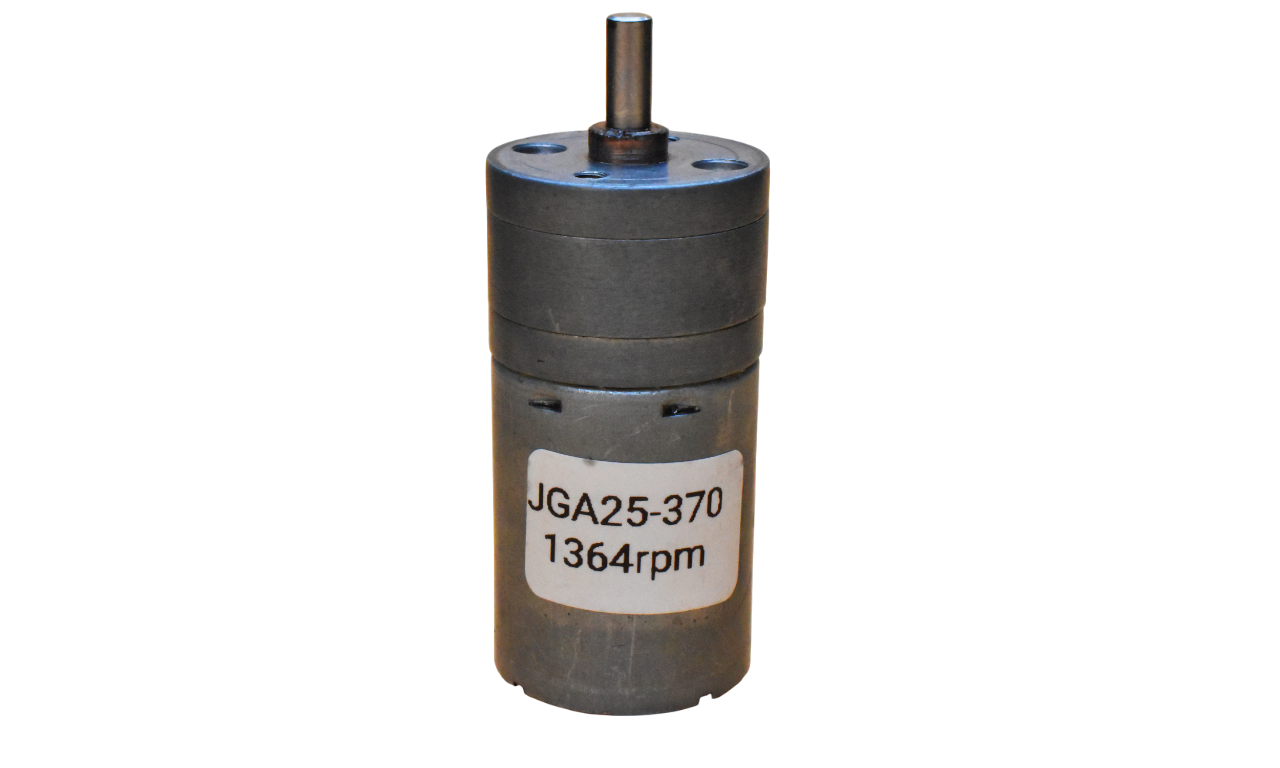
\includegraphics[width=\textwidth]{images/moteur_jga25-370 1364.png}
        \caption{Moteur JGA25}
    \end{subfigure}
    \hfill
    \begin{subfigure}[b]{0.19\textwidth}
        \centering
        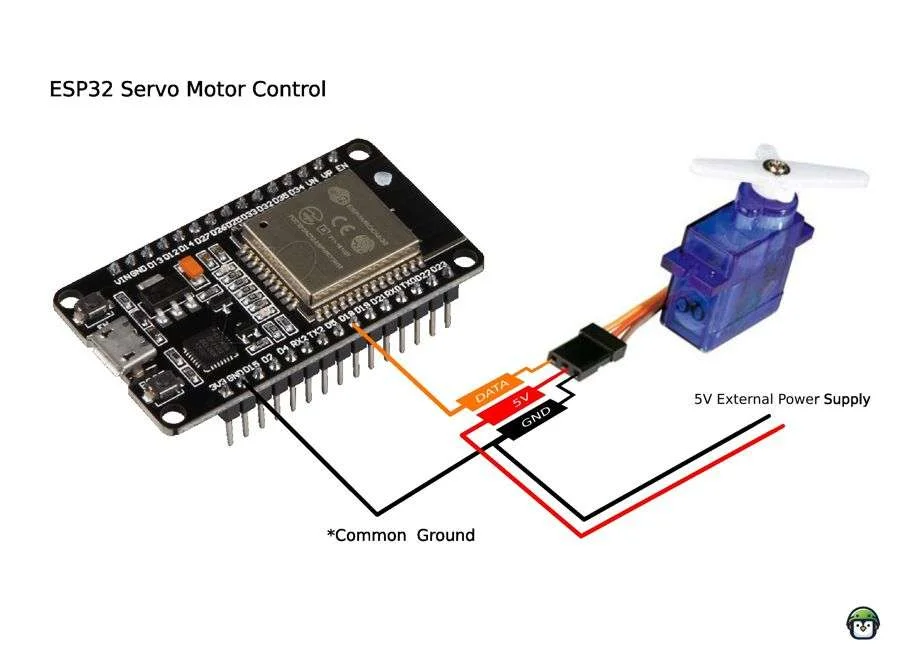
\includegraphics[width=\textwidth]{images/samgalope.dev-devdigest-ESP32-SERVO-SG90.png}
        \caption{Servo SG90}
    \end{subfigure}
    \hfill
    \begin{subfigure}[b]{0.19\textwidth}
        \centering
        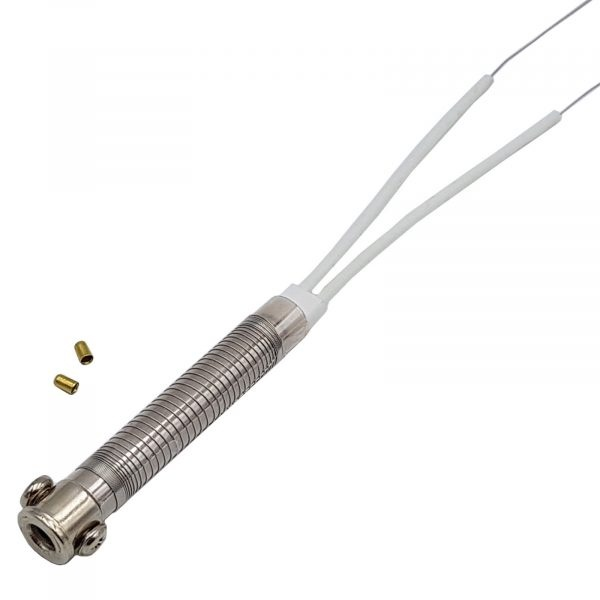
\includegraphics[width=\textwidth]{images/resistance_chauffante.jpg}
        \caption{Résistance}
    \end{subfigure}
    \hfill
    \begin{subfigure}[b]{0.19\textwidth}
        \centering
        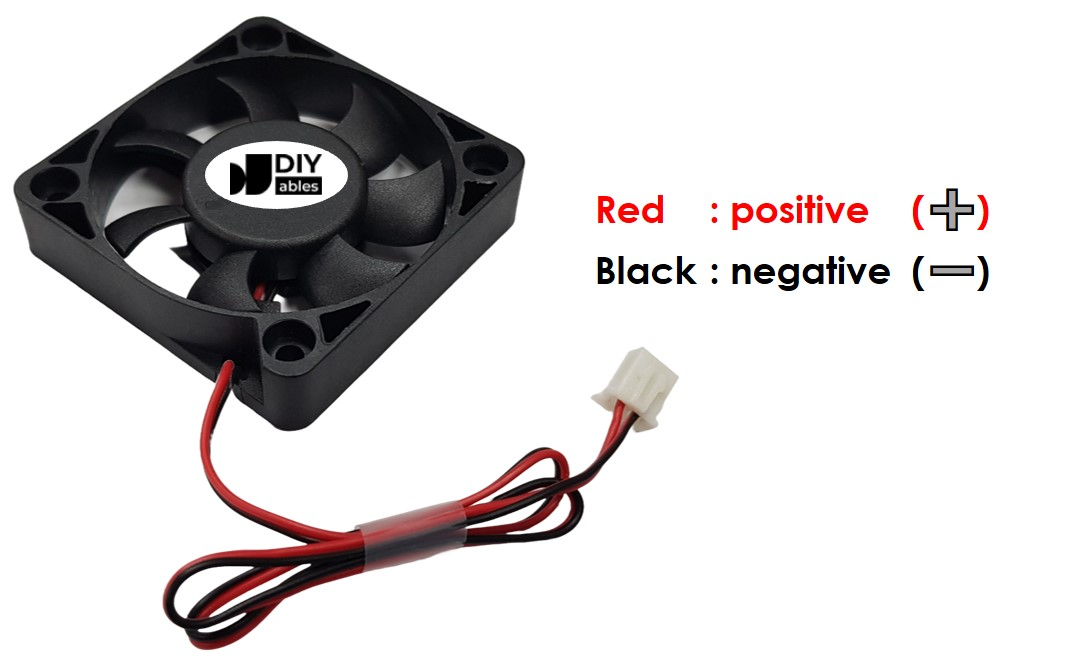
\includegraphics[width=\textwidth]{images/fan-pinout.jpg}
        \caption{Ventilateur}
    \end{subfigure}
    \hfill
    \begin{subfigure}[b]{0.19\textwidth}
        \centering
        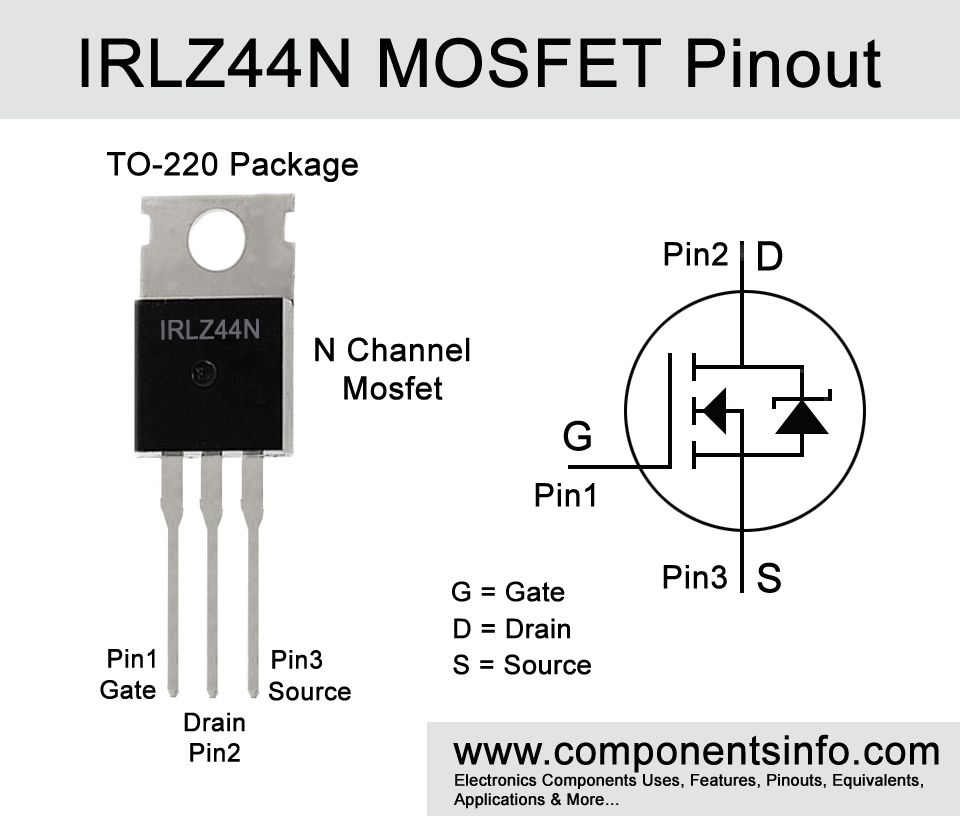
\includegraphics[width=\textwidth]{images/irlz44n-pinout-equivalent.png}
        \caption{MOSFET}
    \end{subfigure}
    \caption{Actionneurs et interface de puissance du système}
    \label{fig:actionneurs_systeme}
\end{figure}
\FloatBarrier

Le \textbf{MOSFET IRLZ44N} est retenu car, contrairement aux MOSFET standards nécessitant 10~V de commande, ce modèle \textit{Logic Level} se sature directement avec les 3,3~V de l'ESP32. Il peut commuter jusqu'à 47~A avec une résistance interne de seulement 0,022~$\Omega$, permettant un pilotage PWM précis des moteurs et de la résistance chauffante sans échauffement excessif \cite{irlz44n_datasheet}. Il convient de noter que la valeur de 175~W indiquée dans le Tableau~\ref{tab:specs_actionneurs} correspond à la puissance maximale absolue que ce composant est physiquement capable de dissiper (selon sa fiche technique, sous conditions de refroidissement optimal), et non à la puissance effectivement consommée par le prototype SMART-SOJA dont le bilan total s'élève à 37,85~W (Tableau~\ref{tab:specs_energie}).

\subsection{Interfaces homme-machine et traçabilité locale}

\begin{table}[H]
    \caption{Interfaces locales et modules de traçabilité}
    \label{tab:specs_ihm}
    \centering
    \small
    \renewcommand{\arraystretch}{1.6}
    \rowcolors{2}{white}{lightGray}
    \begin{tabularx}{\textwidth}{|L|>{\bfseries}C|L|}
        \hline
        \rowcolor{lightGray}
        \textbf{Périphérique} & \textbf{Protocole} & \textbf{Rôle fonctionnel} \\ \hline
        LCD 16×2 & I2C & Affichage en temps réel des métriques et états du système. \\ \hline
        Lecteur MicroSD & SPI & Enregistrement local des données en mode \textit{Store-and-Forward}. \\ \hline
        Potentiomètres ($\times 2$) & ADC (12 bits) & Réglage manuel de la vitesse des moteurs par l'opérateur. \\ \hline
        Boutons ON/OFF & GPIO Pull-Up & Démarrage et arrêt sécurisé du cycle de traitement. \\ \hline
        LEDs \& Buzzer & Digital/PWM & Signalisation d'état (mode, alerte, erreur). \\ \hline
    \end{tabularx}
\end{table}

Le système intègre également des interfaces de dialogue local (Figure \ref{fig:ihm_systeme}) pour l'opérateur de terrain.

\begin{figure}[H]
    \centering
    \begin{subfigure}[b]{0.19\textwidth}
        \centering
        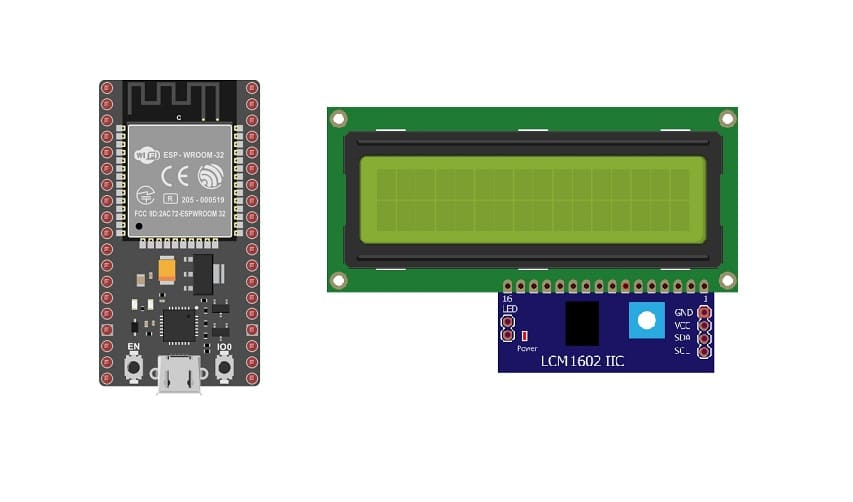
\includegraphics[width=\textwidth]{images/esp32-lcd-i2c-single.jpg}
        \caption{LCD 16x2}
    \end{subfigure}
    \hfill
    \begin{subfigure}[b]{0.19\textwidth}
        \centering
        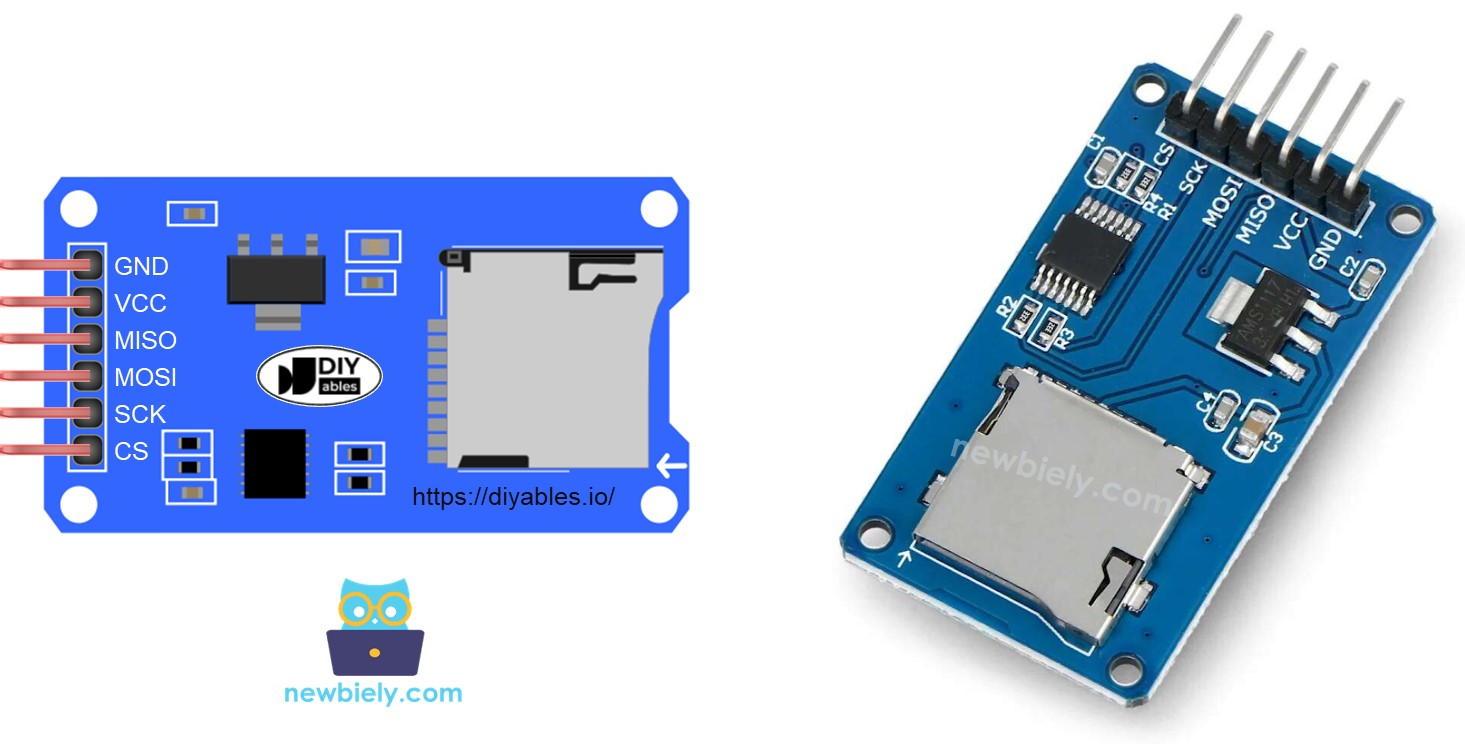
\includegraphics[width=\textwidth]{images/micro-sd-card-module-pinout.jpg}
        \caption{Lecteur SD}
    \end{subfigure}
    \hfill
    \begin{subfigure}[b]{0.19\textwidth}
        \centering
        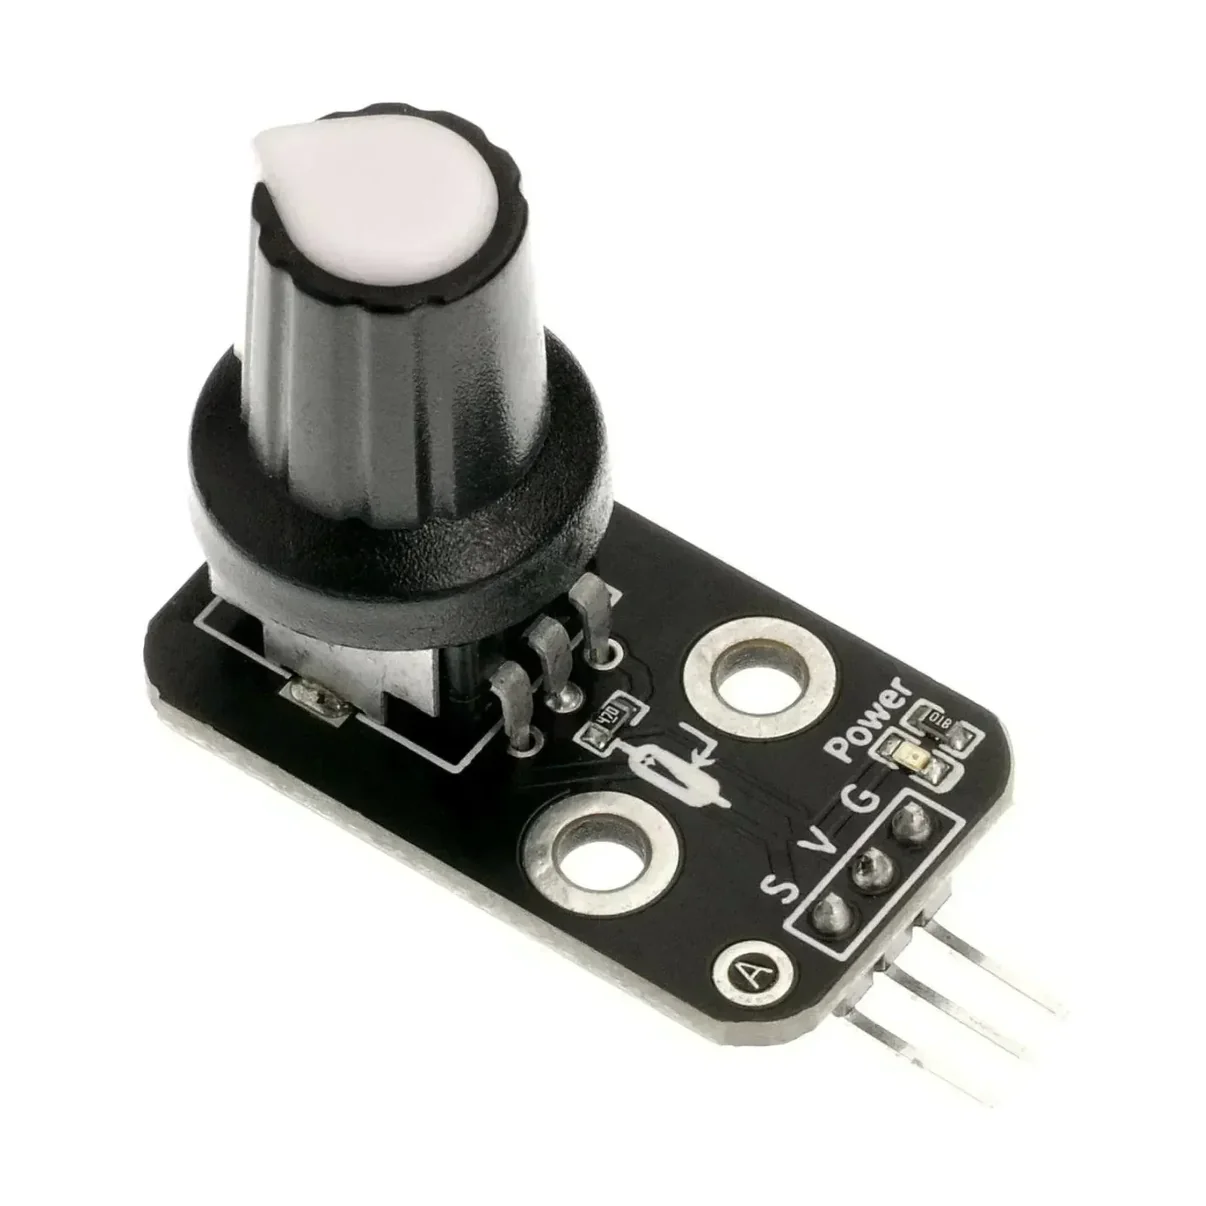
\includegraphics[width=\textwidth]{images/potentiometre_rotatif.png}
        \caption{Potentiomètre}
    \end{subfigure}
    \hfill
    \begin{subfigure}[b]{0.19\textwidth}
        \centering
        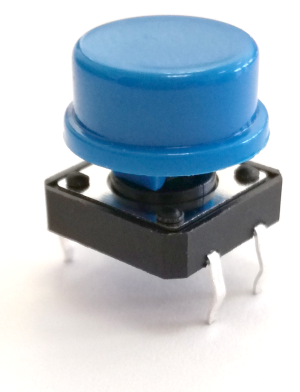
\includegraphics[width=\textwidth]{images/bouton_bleu.png}
        \caption{Boutons}
    \end{subfigure}
    \hfill
    \begin{subfigure}[b]{0.19\textwidth}
        \centering
        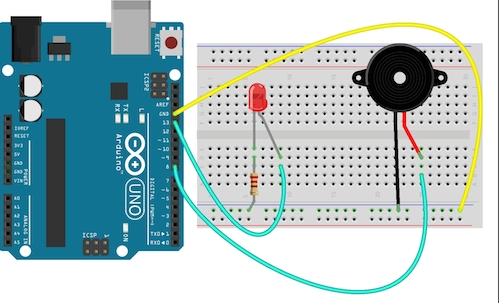
\includegraphics[width=\textwidth]{images/buzzer + led.jpg}
        \caption{Signalisation}
    \end{subfigure}
    \caption{Interfaces locales et modules de traçabilité}
    \label{fig:ihm_systeme}
\end{figure}
\FloatBarrier

Le \textbf{lecteur MicroSD} (interface SPI, format FAT32) joue un rôle critique pour la traçabilité : en l'absence de réseau WiFi, toutes les métriques de traitement sont sauvegardées localement et retransmises automatiquement au broker MQTT dès la reconnexion — mécanisme dit de \textit{Store-and-Forward}.

% -------------------------------------------------------
\section{Sous-système énergétique : autonomie solaire}
% -------------------------------------------------------
Pour garantir un fonctionnement ininterrompu en milieu rural hors réseau, le système \textbf{SMART-SOJA} repose sur une alimentation photovoltaïque dimensionnée selon les principes de calcul de capacité batterie pour systèmes isolés \cite{labouret2017}. Le bilan de puissance des actionneurs est détaillé dans le Tableau \ref{tab:specs_energie} et le synoptique complet de la chaîne de puissance est présenté en \textbf{Annexe \ref{annexe:schema_alim}}.

\begin{table}[H]
    \caption{Bilan énergétique et spécifications d'alimentation}
    \label{tab:specs_energie}
    \centering
    \small
    \renewcommand{\arraystretch}{1.5}
    \rowcolors{2}{white}{lightGray}
    \begin{tabularx}{\textwidth}{|L|L|}
        \hline
        \rowcolor{lightGray}
        \textbf{Paramètre Énergétique} & \textbf{Valeur / Spécification} \\ \hline
        Production (Panneau) & Monocristallin 50~W (Peak) \\ \hline
        Stockage (Batterie) & Plomb-acide 12~V 20~Ah (240~Wh) \\ \hline
        Bilan de puissance crête & 37,85~W (Toutes charges ON) \\ \hline
        Consommation journalière est. & environ 113,5~Wh (pour 3h de travail) \\ \hline
        Autonomie théorique (sans soleil) & environ 1 jour (à 50\% de décharge) \\ \hline
        Conversion & Régulateurs Buck LM2596 (Efficacité > 85\%) \\ \hline
    \end{tabularx}
\end{table}

\textbf{Dimensionnement du système :} Pour valider les choix technologiques du kit de l'entreprise \textbf{QOTTO} (Batterie de 20~Ah et panneau de 50~W), nous avons procédé à un dimensionnement basé sur le besoin réel du prototype.

\begin{enumerate}
    \item \textbf{Étape 1 — Bilan de puissance crête :} La puissance totale est la somme des consommations réelles des composants du prototype (incluant deux résistances et deux ventilateurs pour le séchage) :
    \[ P_{tot} = \underbrace{9,0\text{W}}_{\text{2 Moteurs}} + \underbrace{\mathbf{24,0\text{W}}}_{\text{2 Résistances}} + \underbrace{\mathbf{3,6\text{W}}}_{\text{2 Ventilos}} + \underbrace{1,25\text{W}}_{\text{ESP32}} = \mathbf{37,85~\text{W}} \]
    
    \item \textbf{Étape 2 — Énergie consommée par jour ($E_j$) :} En considérant une utilisation du prototype pendant \textbf{3 heures par jour} (soit environ 18 cycles de traitement), l'énergie totale consommée est :
    \[ E_{jour} = 37,85~\text{W} \times 3~\text{h} \approx \mathbf{113,5~\text{Wh/jour}} \]
    
    \item \textbf{Étape 3 — Validation de la batterie :} La batterie de 12~V et 20~Ah possède une capacité totale de \textbf{240~Wh}. En limitant la décharge à 50~\% pour prolonger sa durée de vie (standard pour les batteries au plomb), l'énergie réellement disponible est de \textbf{120~Wh}.
    \begin{itemize}
        \item \textbf{Conclusion :} 120~Wh (disponibles) $>$ 113,5~Wh (besoin), la batterie est donc bien dimensionnée pour couvrir une session de travail quotidienne en autonomie.
    \end{itemize}

    \item \textbf{Étape 4 — Validation du panneau solaire :} Avec un ensoleillement moyen de 5 heures par jour au Bénin, le panneau de 50~W produit :
    \[ E_{produite} = 50~\text{W} \times 5~\text{h} = \mathbf{250~\text{Wh/jour}} \]
    \begin{itemize}
        \item \textbf{Conclusion :} 250~Wh (produits) $>$ 113,5~Wh (besoin), le panneau recharge la batterie très facilement, offrant une marge de sécurité confortable pour compenser les jours de faible ensoleillement.
    \end{itemize}
\end{enumerate}

% -------------------------------------------------------
\section{Sous-système mécanique : architecture modulaire}
% -------------------------------------------------------
La conception mécanique repose sur une structure modulaire composée d'un châssis porteur accueillant quatre blocs fonctionnels amovibles. Les matériaux ont été sélectionnés selon un compromis robustesse/coût de prototypage (Tableau \ref{tab:specs_mecanique}). Des photographies des matériaux bruts utilisés sont consultables en \textbf{Annexe \ref{annexe:materiaux_mecaniques}}.

\begin{table}[H]
    \caption{Spécifications mécaniques, contraintes et justification des matériaux}
    \label{tab:specs_mecanique}
    \centering
    \small
    \renewcommand{\arraystretch}{1.5}
    \rowcolors{2}{white}{lightGray}
    \begin{tabularx}{\textwidth}{|L|C|L|L|}
        \hline
        \rowcolor{lightGray}
        \textbf{Élément} & \textbf{Masse (kg)} & \textbf{Contrainte / Rigidité} & \textbf{Justification Matériau} \\ \hline
        Châssis porteur & 12,0 & Compression / Haute & Acier (Tubes 40~mm) : Robustesse et soudabilité \\ \hline
        Support Tamis & 0,293 & Vibration / Haute & Inox 304 : Résistance à la corrosion et hygiène \\ \hline
        Support Capteur & 0,1 & Flexion / Moyenne & PLA (3D) : Précision et légèreté \\ \hline
        Roulettes (×4) & 2,0 & Chocs / Élastique & Caoutchouc HD : Absorption des vibrations \\ \hline
    \end{tabularx}
\end{table}
\FloatBarrier

Les quatre blocs fonctionnels (alimentation, nettoyage, séchage et pesée) sont conçus pour être retirés individuellement du châssis. Ce système de glissières et connecteurs rapides facilite grandement la maintenance en milieu rural, évitant ainsi le démontage intégral de la machine.



% -------------------------------------------------------
\section{Méthodologie logicielle : contrôle temps réel}
% -------------------------------------------------------

\subsection{Le système multitâche FreeRTOS}
La gestion simultanée de la sécurité, du contrôle et de la communication Internet des objets sur l'ESP32 nécessite un ordonnancement rigoureux des tâches. Nous utilisons \textbf{FreeRTOS} \cite{freeRTOS}, un noyau temps réel miniature qui offre :
\begin{itemize}
    \item \textbf{Déterminisme :} La lecture des capteurs et le pilotage des actionneurs ne sont jamais interrompus par les tâches réseau.
    \item \textbf{Gestion Multi-Core :} Les deux cœurs de l'ESP32 sont répartis selon la criticité des tâches.
    \item \textbf{Hiérarchie des priorités :} Les tâches de sécurité préemptent systématiquement toutes les autres.
\end{itemize}

Cette organisation logicielle est détaillée dans le Tableau \ref{tab:freertos_sched}.

\begin{table}[H]
    \caption{Hiérarchie et configuration de l'ordonnanceur FreeRTOS}
    \label{tab:freertos_sched}
    \centering
    \small
    \renewcommand{\arraystretch}{1.5}
    \rowcolors{2}{white}{lightGray}
    \begin{tabularx}{\textwidth}{|L|C|L|L|}
        \hline
        \rowcolor{lightGray}
        \textbf{Tâche} & \textbf{Priorité} & \textbf{Justification} & \textbf{Risque en cas de latence} \\ \hline
        \textbf{Task\_Safety} & 4 (Max) & Sécurité critique (Arrêt, Surchauffe) & Endommagement du matériel \\ \hline
        \textbf{Task\_Control} & 3 (Haute) & Ordonnancement GRAFCET & Conflits d'états et blocages \\ \hline
        \textbf{Task\_Sensing} & 2 (Moy.) & Acquisition capteurs (Filtrage) & Mesures erronées ou bruitées \\ \hline
        \textbf{Task\_Actuators} & 2 (Moy.) & Pilotage PWM et Servomoteurs & Réactivité saccadée \\ \hline
        \textbf{Task\_LCD} & 1 (Faible) & Interface locale (I2C) & Affichage figé (non critique) \\ \hline
        \textbf{Task\_MQTT} & 1 (Faible) & Communication Internet des objets et SD & Perte de traçabilité \\ \hline
    \end{tabularx}
\end{table}

Le chronogramme de la Figure \ref{fig:freertos_chronogramme} illustre la dynamique de l'ordonnancement préemptif sur l'ESP32.

\begin{figure}[H]
    \centering
    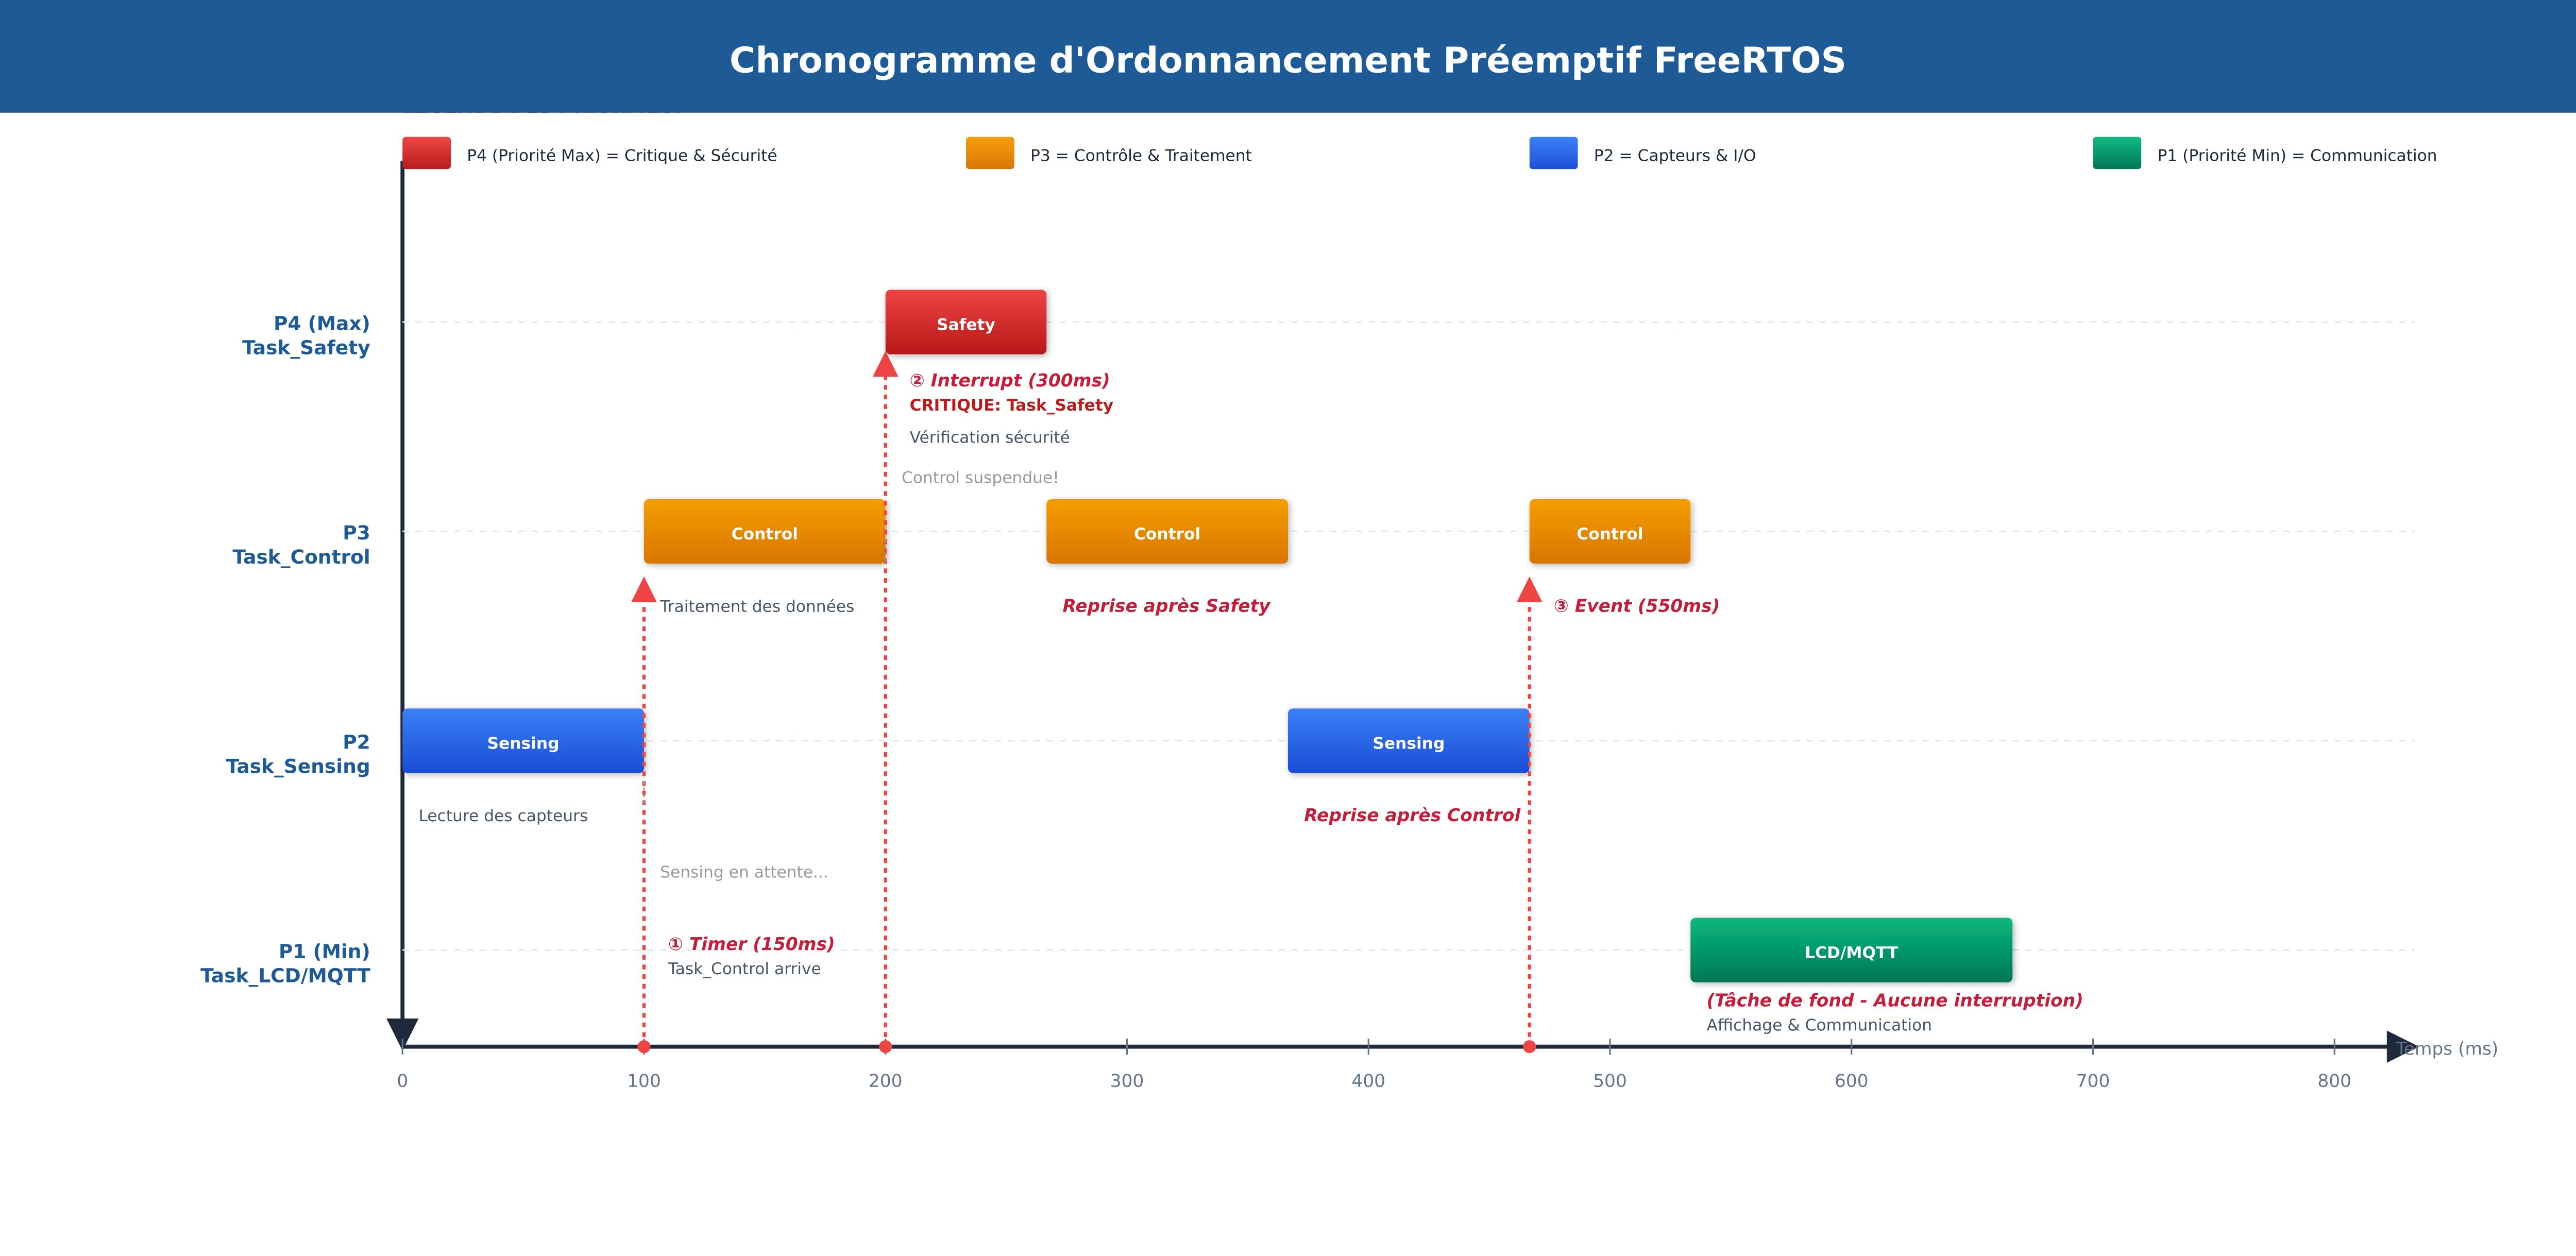
\includegraphics[width=\textwidth]{images/freertos_chronogramme.png}
    \caption{Chronogramme d'ordonnancement préemptif FreeRTOS : Illustration de la préemption et de la hiérarchie des priorités}
    \label{fig:freertos_chronogramme}
\end{figure}

L'ordonnancement repose sur trois principes fondamentaux illustrés par ce graphique :
\begin{enumerate}
    \item \textbf{La Préemption (Interruption) :} Toute tâche de priorité supérieure (ex: \textit{Task\_Safety}) suspend immédiatement l'exécution de la tâche courante (ex: \textit{Task\_Control}), garantissant une réactivité immédiate aux événements critiques.
    \item \textbf{La Reprise Automatique :} Lorsqu'une tâche prioritaire se bloque ou se termine, le noyau FreeRTOS restaure le contexte de la tâche précédemment suspendue, qui reprend exactement là où elle s'était arrêtée.
    \item \textbf{La Gestion des Priorités :} Les tâches de faible priorité (ex: \textit{Task\_LCD / Task\_MQTT}) ne s'exécutent que si aucune tâche plus prioritaire n'est prête à fonctionner, optimisant l'usage du processeur pour les fonctions vitales du système.
\end{enumerate}

\subsection{Modélisation de l'automatisme : le GRAFCET}

La complexité du cycle de traitement du soja — combinant tri mécanique, séchage thermique et pesage électronique — nécessite un outil de modélisation robuste pour garantir une exécution séquentielle sans conflit d'actionneurs. Pour ce faire, nous avons retenu le formalisme du \textbf{GRAFCET} (Graphe Fonctionnel de Commande Étape-Transition), décliné en deux niveaux d'analyse.

\subsubsection{Analyse fonctionnelle (GRAFCET niveau 1)}

Le GRAFCET de niveau 1 décrit le comportement global du système SMART-SOJA du point de vue de l'utilisateur. Le cycle se décompose en trois phases majeures :
\begin{itemize}
    \item \textbf{Phase de préparation :} Le système vérifie la disponibilité de la matière première (Trémie) et la présence d'un réceptacle (Sac) avant d'autoriser l'admission des grains.
    \item \textbf{Phase de traitement :} Elle englobe le nettoyage granulométrique par vibration, suivi d'une analyse critique de l'humidité. Si le soja dépasse le seuil de 12~\%, une séquence de séchage et de brassage est activée de manière itérative jusqu'à conformité.
    \item \textbf{Phase de clôture :} Le lot est transféré vers l'unité de pesée, les données de traçabilité sont enregistrées et le système attend le retrait du sac pour se réinitialiser.
\end{itemize}

\subsubsection{Analyse technologique (GRAFCET niveau 2)}

Le passage au niveau 2 permet de traduire les fonctions précédentes en ordres pilotables par le microcontrôleur ESP32. Cette étape définit les interfaces matérielles :
\begin{itemize}
    \item \textbf{Gestion des entrées :} Utilisation de capteurs infrarouges (IR1 et IR2) pour la détection de présence, et de sondes capacitives reliées aux convertisseurs analogique-numérique (ADC) pour l'humidité.
    \item \textbf{Pilotage des sorties :} Commande de servomoteurs par signaux PWM pour la gestion des vannes, et activation de MOSFETs de puissance pour les éléments thermiques et vibratoires.
\end{itemize}

\subsubsection{Évolutions et logique de cycle}

Pour optimiser le rendement énergétique et la qualité, l'automatisme intègre des structures algorithmiques avancées :
\begin{enumerate}
    \item \textbf{Saut de Séquence :} Si le soja est détecté comme étant déjà sec lors de l'analyse initiale, le système court-circuite l'étape de séchage pour passer directement à l'ensachage, économisant ainsi l'énergie des batteries.
    \item \textbf{Reprise de Séquence (Boucle) :} Un rebouclage est systématiquement effectué après chaque phase de séchage vers l'étape d'analyse, garantissant que seuls les grains conformes à la norme NB 01.07.004 quittent la machine.
    \item \textbf{Sûreté de fonctionnement :} Une évolution parallèle logicielle surveille en permanence le bouton d'arrêt d'urgence et les courants de fuite, capable d'interrompre le cycle à n'importe quelle étape.
\end{enumerate}

\FloatBarrier

\textbf{Double validation de l'humidité :} L'ensachage n'est autorisé que si les deux sondes Soil1 \textit{ET} Soil2 confirment individuellement $H \leq 12~\%$. Cette double validation prévient les hétérogénéités verticales du lot et les défauts de capteur isolé :
\begin{align*}
\text{Sortie\_séchage} &= (S_1 \leq 12~\%) \text{ ET } (S_2 \leq 12~\%) \\
\text{Déclenchement\_séchage} &= (S_1 > 12~\%) \text{ OU } (S_2 > 12~\%)
\end{align*}

L'ensemble de ces règles logiques et technologiques est synthétisé dans le GRAFCET de la Figure \ref{fig:grafcet_systeme}.

\begin{figure}[H]
    \centering
    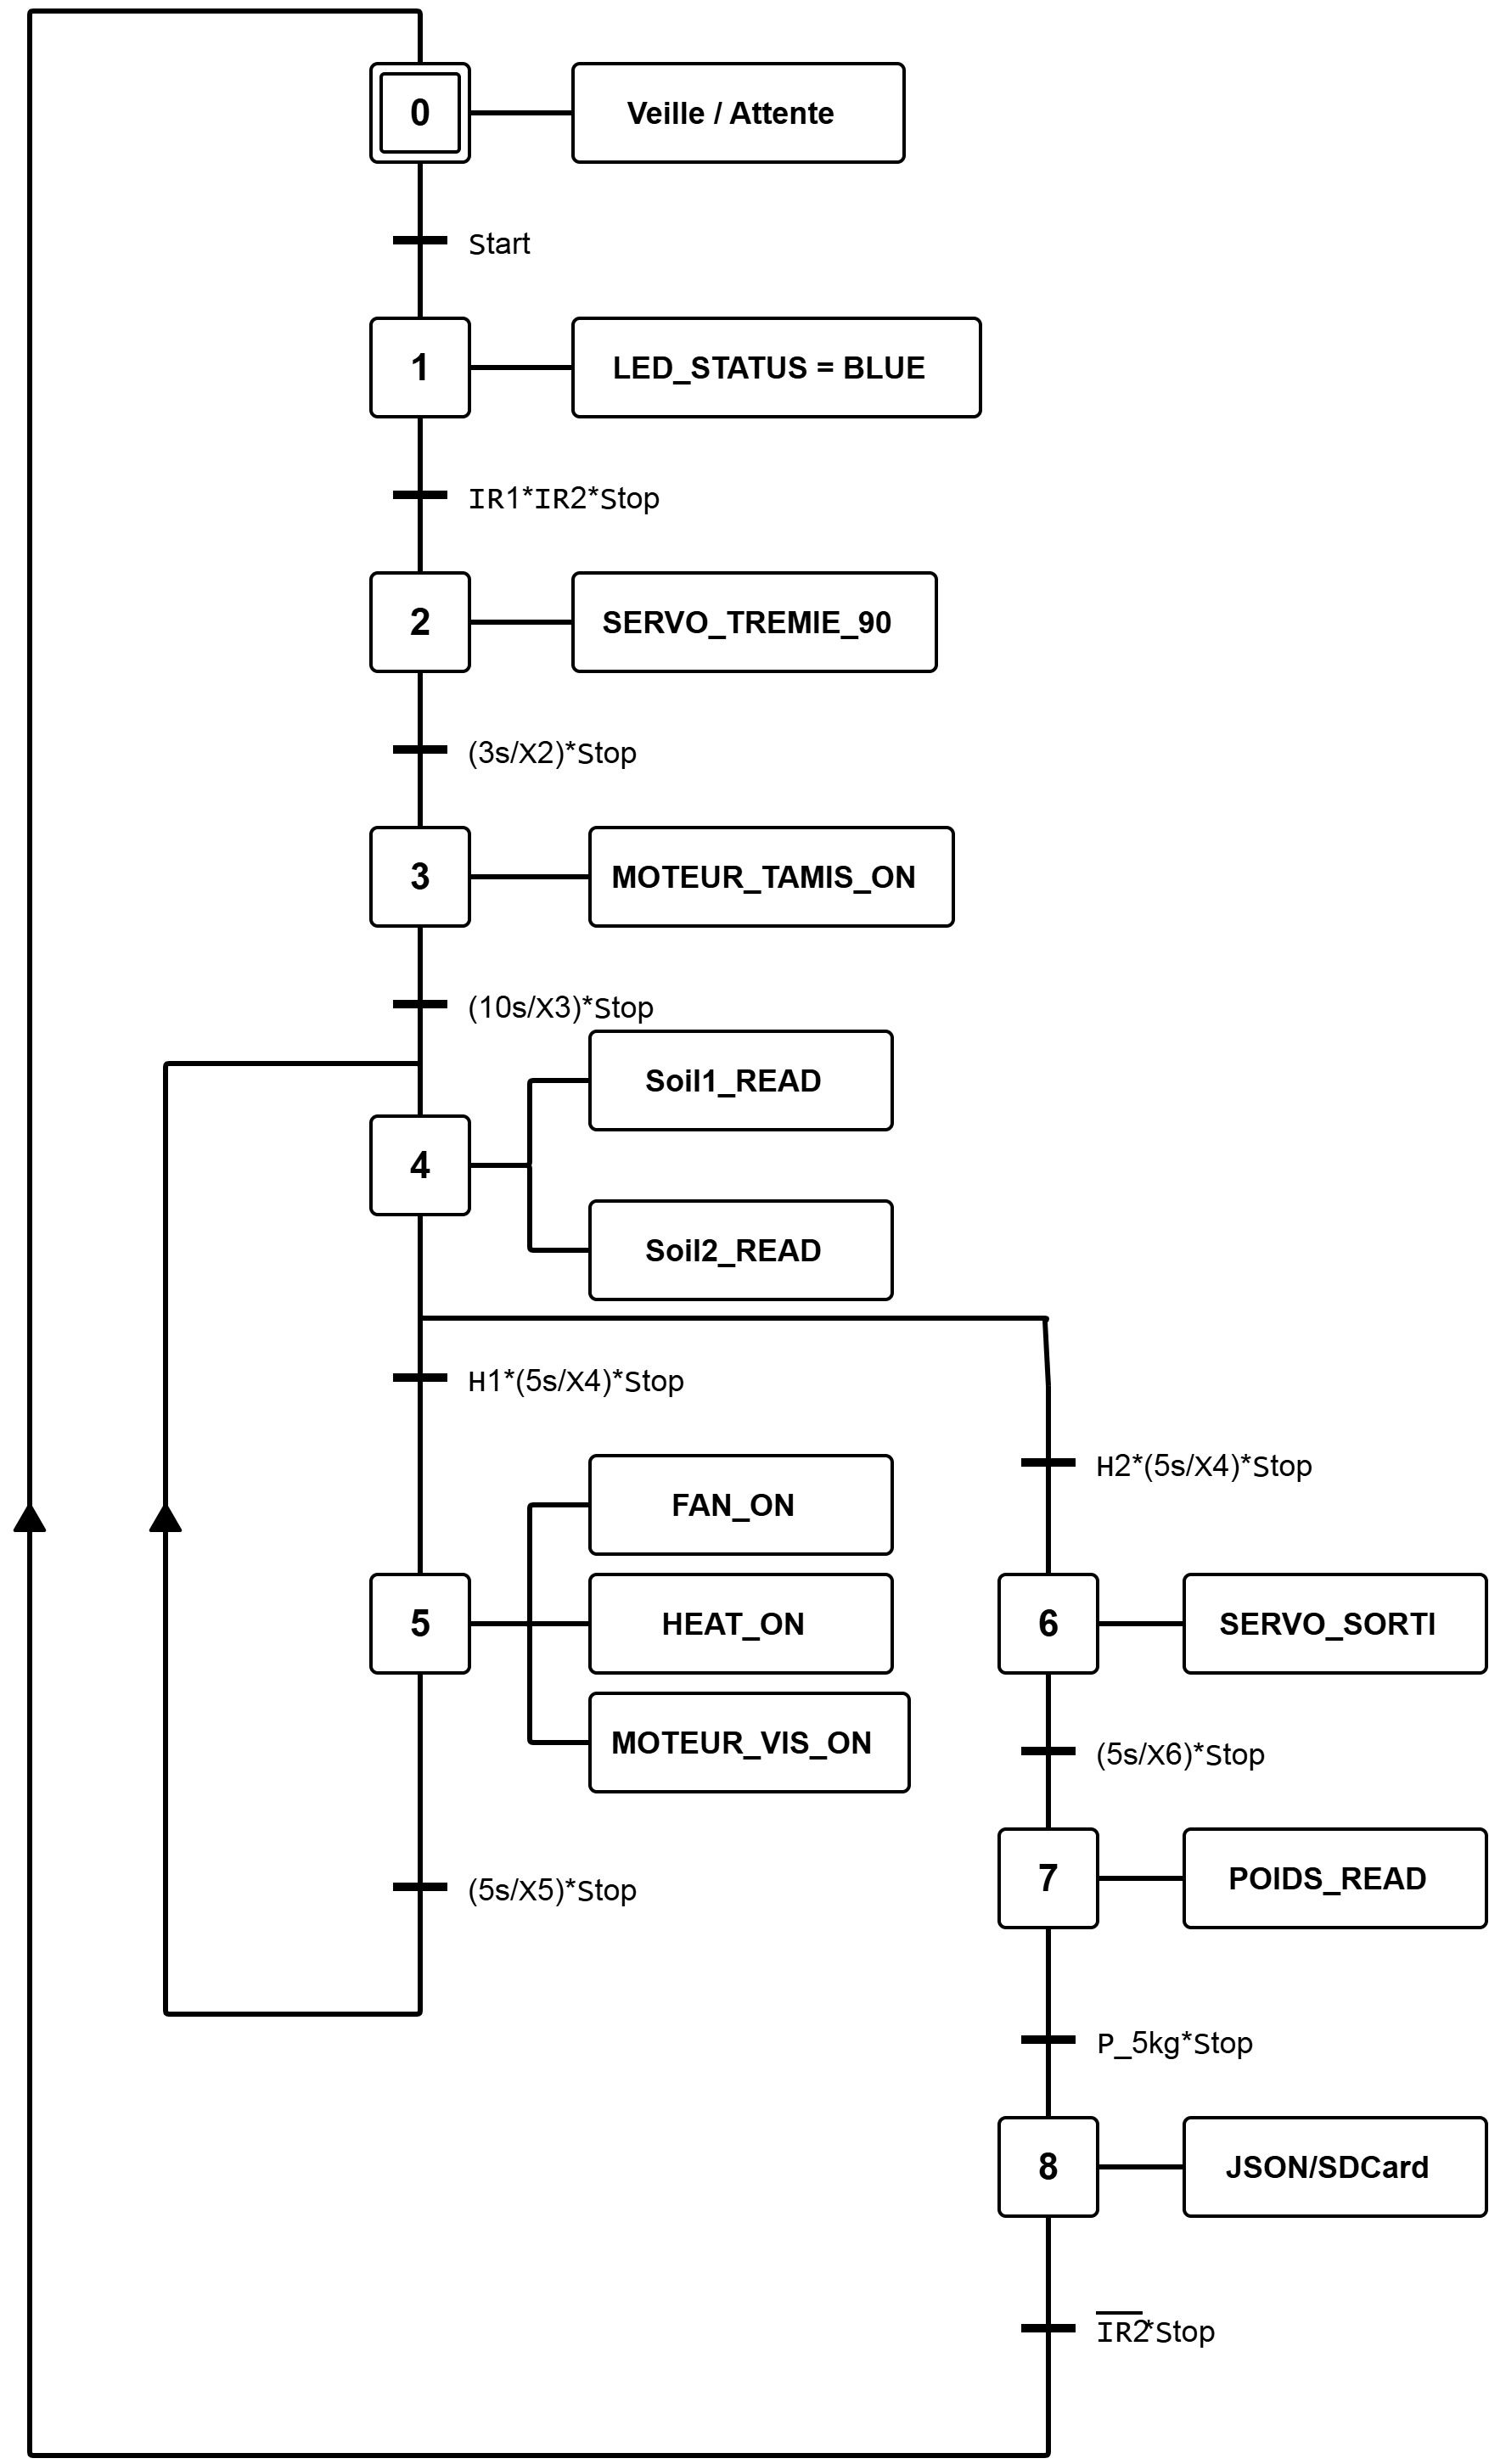
\includegraphics[width=0.6\textwidth]{images/grafcet_smart.png}
    \caption{Algorithme de contrôle séquentiel du système (GRAFCET Niveau 2)}
    \label{fig:grafcet_systeme}
\end{figure}


\subsection{Communication et traçabilité numérique}

Une fois le cycle de traitement validé par le GRAFCET, les données doivent être exportées pour assurer la traçabilité du lot. Le protocole \textbf{MQTT} (architecture Publication/Abonnement) est retenu pour sa légèreté et sa robustesse sur les réseaux à faible bande passante \cite{mqtt_org}. L'utilisation du format \textbf{JSON} garantit quant à elle l'interopérabilité des données entre l'Edge et le Cloud \cite{hanes2017}.

À chaque fin de cycle, la machine génère un \textbf{passeport numérique} au format \textbf{JSON}. Ce message regroupe l'ensemble des métriques de traçabilité (identifiant unique, horodatage, humidité moyenne et poids final) et est publié vers le broker central.

En cas de perte de connexion, ces données sont archivées sur la carte MicroSD et renvoyées dès le rétablissement du signal (\textit{Store-and-Forward}).

% Fin de la section méthodes


% -------------------------------------------------------
% PARTIE 3 : CONCEPTION ET IMPLÉMENTATION
% -------------------------------------------------------

% ---- SECTION CONCEPTION ET IMPLÉMENTATION ----

% -------------------------------------------------------
\section{Environnement de conception et de développement}
Pour mener à bien ce projet mécatronique, plusieurs outils professionnels de conception et de développement ont été mobilisés. Ils permettent de garantir la précision des modèles et l'interopérabilité des données.

\subsection{Conception mécanique et électronique}
\begin{itemize}
    \item \textbf{SolidWorks (Dassault Systèmes) :} Utilisé pour la modélisation 3D intégrale du prototype, les simulations d'assemblage et la génération des mises en plan techniques. C'est le standard industriel pour la conception de systèmes mécaniques complexes.
    \item \textbf{KiCad EDA :} Suite logicielle open-source retenue pour la saisie schématique et le routage du PCB. Sa flexibilité et sa gratuité en font un outil idéal pour le prototypage rapide en milieu académique et professionnel.
\end{itemize}

\subsection{Développement logiciel}
\begin{itemize}
    \item \textbf{Arduino IDE :} Utilisé pour le codage, la compilation et le téléversement du firmware sur l'ESP32. Sa vaste bibliothèque de pilotes facilite l'interfaçage des capteurs et la gestion du WiFi.
    \item \textbf{VS Code (Visual Studio Code) :} Retenu pour le développement du tableau de bord Internet des objets (HTML/JS) en raison de sa gestion avancée du versionnement (Git) et de son écosystème d'extensions.
\end{itemize}

\begin{figure}[H]
    \centering
    % Première ligne : Conception
    \begin{subfigure}[b]{0.45\textwidth}
        \centering
        
\includegraphics[height=3cm]{images/logo_solidwork.png}
        \caption{SolidWorks (CAO)}
    \end{subfigure}
    \hfill
    \begin{subfigure}[b]{0.45\textwidth}
        \centering
        
\includegraphics[height=3cm]{images/logo_kicad.png}
        \caption{KiCad (EDA)}
    \end{subfigure}
    
    \vspace{0.8cm}
    
    % Deuxième ligne : Développement
    \begin{subfigure}[b]{0.45\textwidth}
        \centering
        
\includegraphics[height=3cm]{images/logo_arduino.png}
        \caption{Arduino IDE (Firmware)}
    \end{subfigure}
    \hfill
    \begin{subfigure}[b]{0.45\textwidth}
        \centering
        
\includegraphics[height=3cm]{images/Visual-Studio-Code-logo.png}
        \caption{VS Code (Tableau de bord IoT)}
    \end{subfigure}
    \caption{Écosystème logiciel utilisé pour le projet SMART-SOJA}
    \label{fig:logos_logiciels}
\end{figure}
\FloatBarrier

\section{Conception électronique : le circuit imprimé (PCB)}

Le schéma électronique global, regroupant l'ensemble des blocs fonctionnels, est consultable en \textbf{Annexe \ref{annexe:schema_global}}.

\subsection{Segmentation fonctionnelle de la conception}
Pour garantir une maintenance aisée et minimiser les interférences électromagnétiques (EMI) entre signaux de puissance et de commande, la conception est segmentée en cinq blocs fonctionnels dès la saisie schématique :

\begin{enumerate}
    \item \textbf{Zone Alimentation (Figure \ref{fig:zone_alim}) :} Régulateur Buck \textbf{LM2596} générant un rail 5~V / 2~A depuis la source 12~V. La logique 3,3~V est assurée par le régulateur interne de l'ESP32.
    \begin{figure}[H]
        \centering
        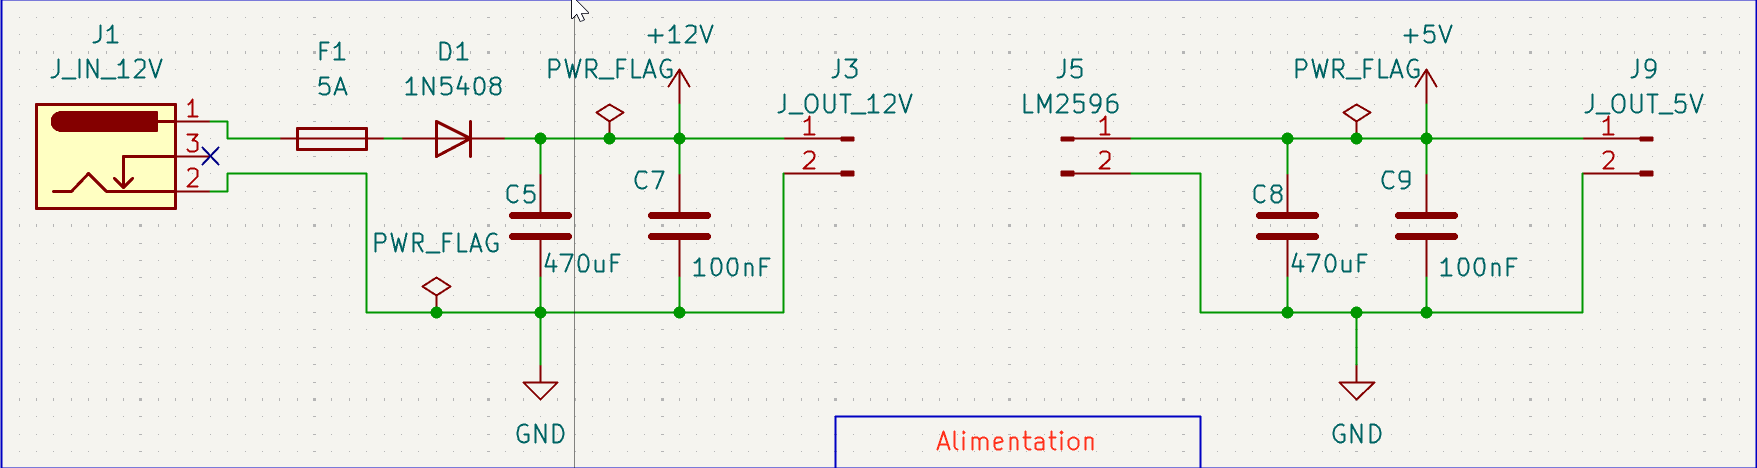
\includegraphics[width=0.55\textwidth]{images/image_circuit_zone-alimentation.PNG}
        \caption{Zone d'alimentation multi-tensions}
        \label{fig:zone_alim}
    \end{figure}

    \item \textbf{Zone ESP32 (Figure \ref{fig:zone_esp32}) :} L'affectation des broches a été optimisée pour éviter les conflits avec les \textit{strapping pins} (GPIO 0, 2, 12, 15) critiques au démarrage.
    \begin{figure}[H]
        \centering
        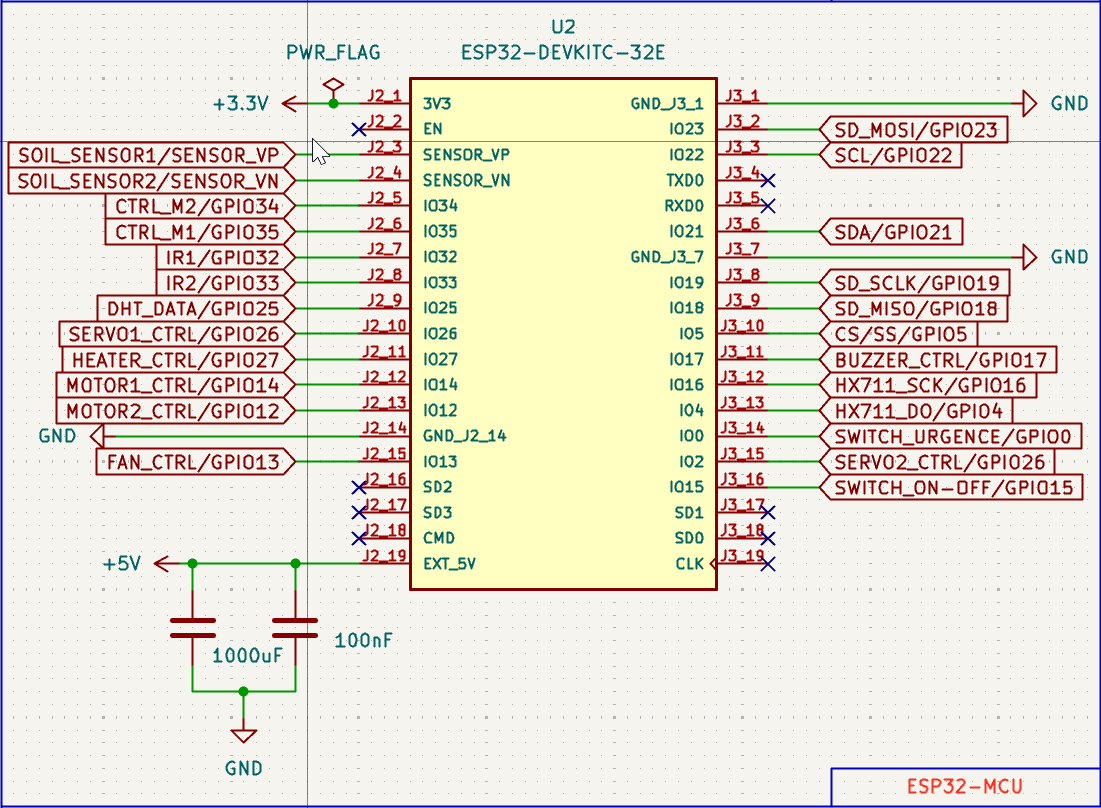
\includegraphics[width=0.55\textwidth]{images/image_circuit_zone-esp32.PNG}
        \caption{Unité de traitement centrale ESP32}
        \label{fig:zone_esp32}
    \end{figure}

    \item \textbf{Zone Puissance (Figure \ref{fig:zone_act}) :} Chaque canal MOSFET IRLZ44N intègre une résistance de grille de 220~$\Omega$, une résistance de rappel pull-down de 10~k$\Omega$ et une diode de roue libre \textbf{1N5408} contre les retours inductifs des moteurs.
    \begin{figure}[H]
        \centering
        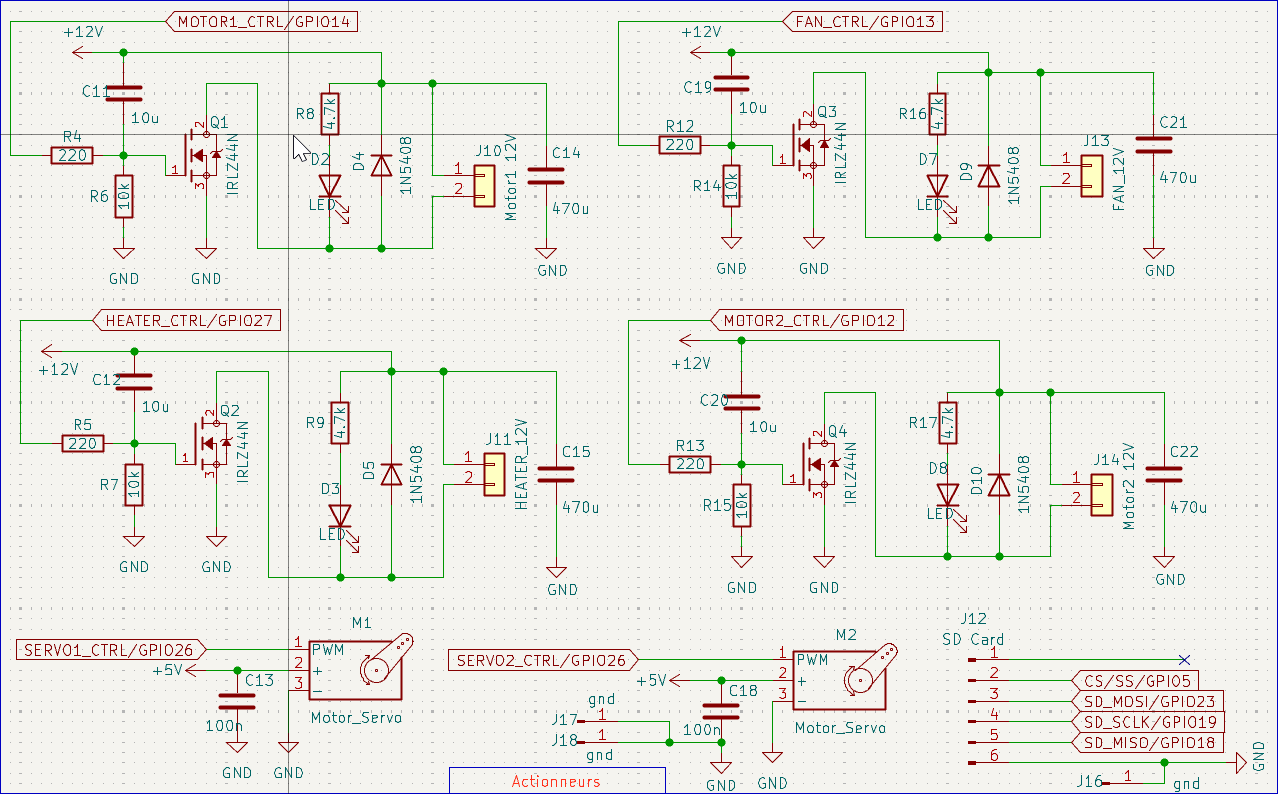
\includegraphics[width=0.55\textwidth]{images/image_circuit_zone-actionneurs.PNG}
        \caption{Étage de puissance avec protections inductives}
        \label{fig:zone_act}
    \end{figure}

    \item \textbf{Zone Acquisition (Figure \ref{fig:zone_cap}) :} Interfaces pour les signaux analogiques (Sondes capacitives sur GPIO 36/39) et numériques (HX711 sur GPIO 25, DHT22, capteurs IR sur GPIO 32/33).
    \begin{figure}[H]
        \centering
        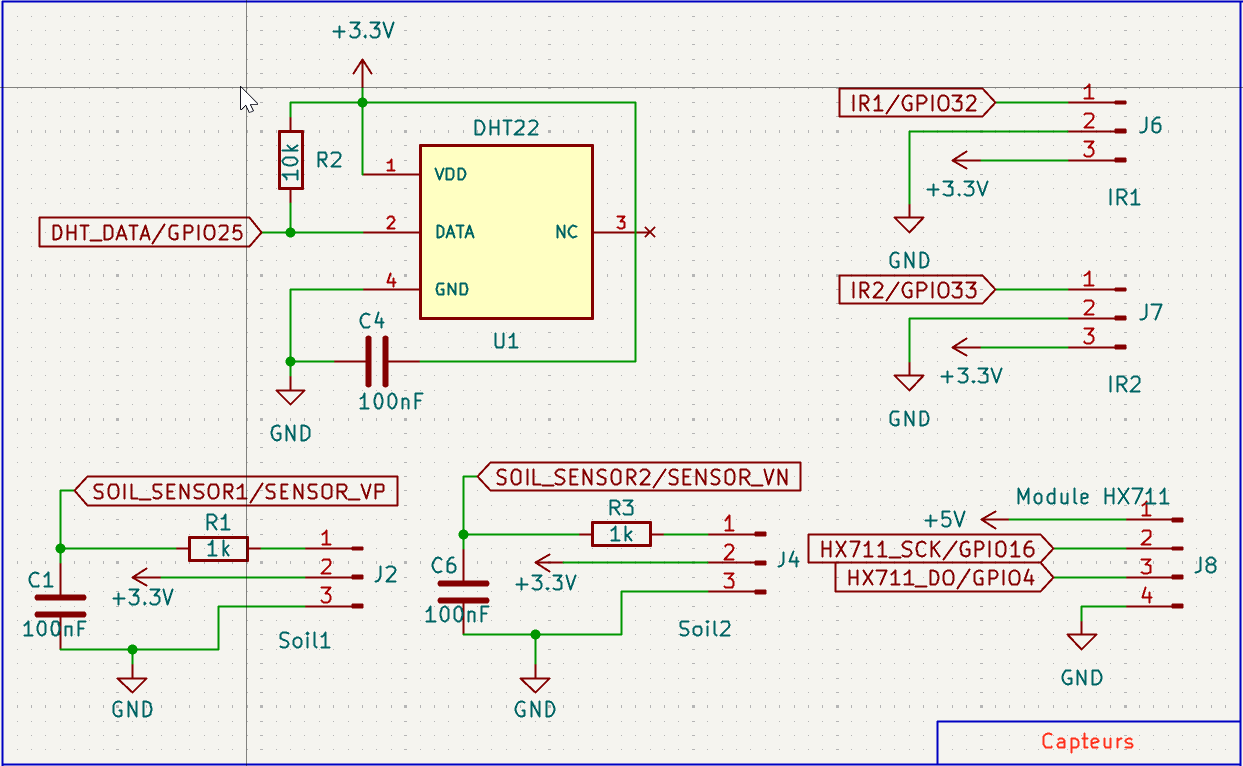
\includegraphics[width=0.55\textwidth]{images/image_circuit_zone-capteurs.PNG}
        \caption{Interface d'acquisition des capteurs}
        \label{fig:zone_cap}
    \end{figure}

    \item \textbf{Zone IHM (Figure \ref{fig:zone_ihm}) :} Gestion du bus I2C (LCD), du bus SPI (carte SD) et des signaux PWM (buzzer, servomoteur, boutons).
    \begin{figure}[H]
        \centering
        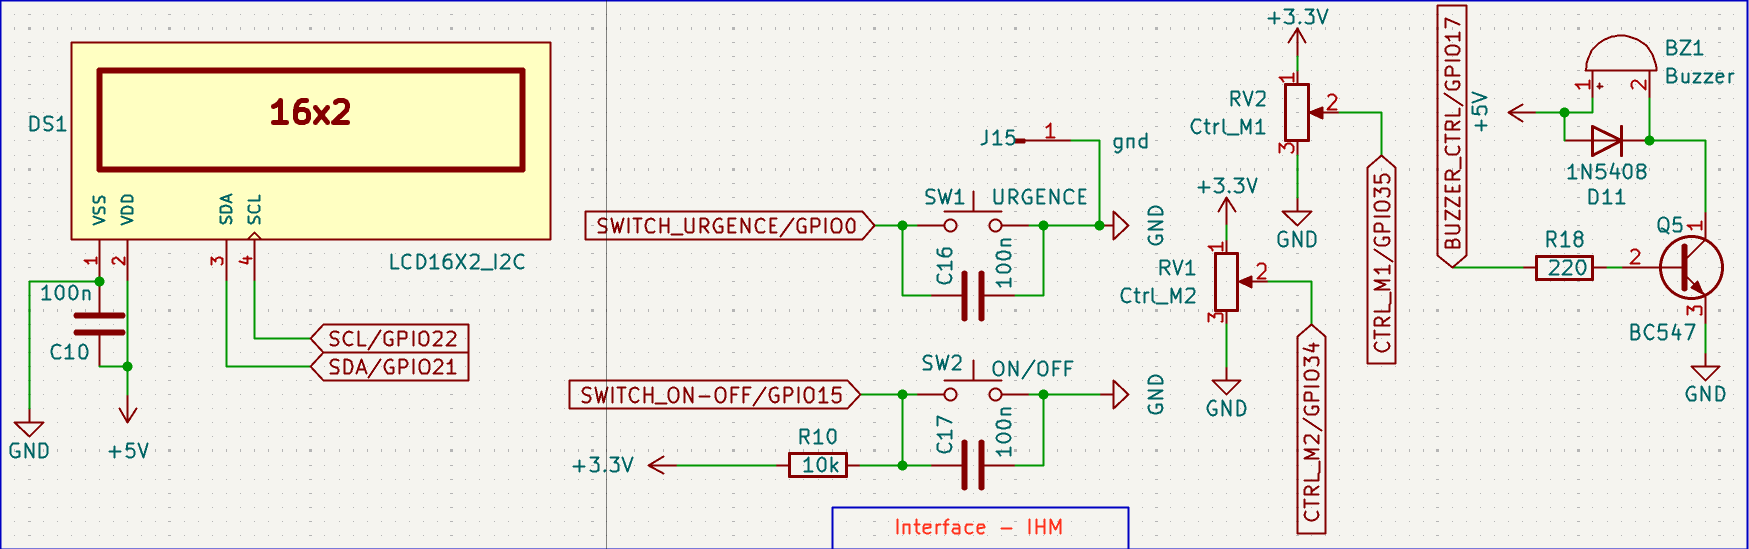
\includegraphics[width=0.55\textwidth]{images/image_circuit_zone-ihm.PNG}
        \caption{Interface Homme-Machine locale}
        \label{fig:zone_ihm}
    \end{figure}
\end{enumerate}
\FloatBarrier

Le routage sous KiCad a été réalisé sur une \textbf{seule couche (Bottom Layer)} pour simplifier la fabrication du prototype. Les pistes de puissance sont dimensionnées à une largeur minimale de \textbf{1~mm} pour supporter les charges inductives sans échauffement. Un plan de masse (Ground Pour) a été généré sur cette face unique pour assurer l'intégrité du signal et limiter les boucles de masse.

La modélisation 3D du PCB a permis de valider l'absence de collision mécanique entre composants volumineux avant fabrication. Les vues détaillées (routage, faces 3D) sont consultables en \textbf{Annexe \ref{annexe:routage_pcb}} et \textbf{Annexe \ref{annexe:vues_3d_pcb}}.

% -------------------------------------------------------
\section{Conception mécanique : architecture modulaire}
% -------------------------------------------------------
La conception mécanique a été réalisée sous \textbf{SolidWorks} selon une architecture modulaire en quatre blocs fonctionnels indépendants (Figure \ref{fig:cad_4blocs}), montés sur un châssis porteur mobile.

\begin{figure}[H]
    \centering
    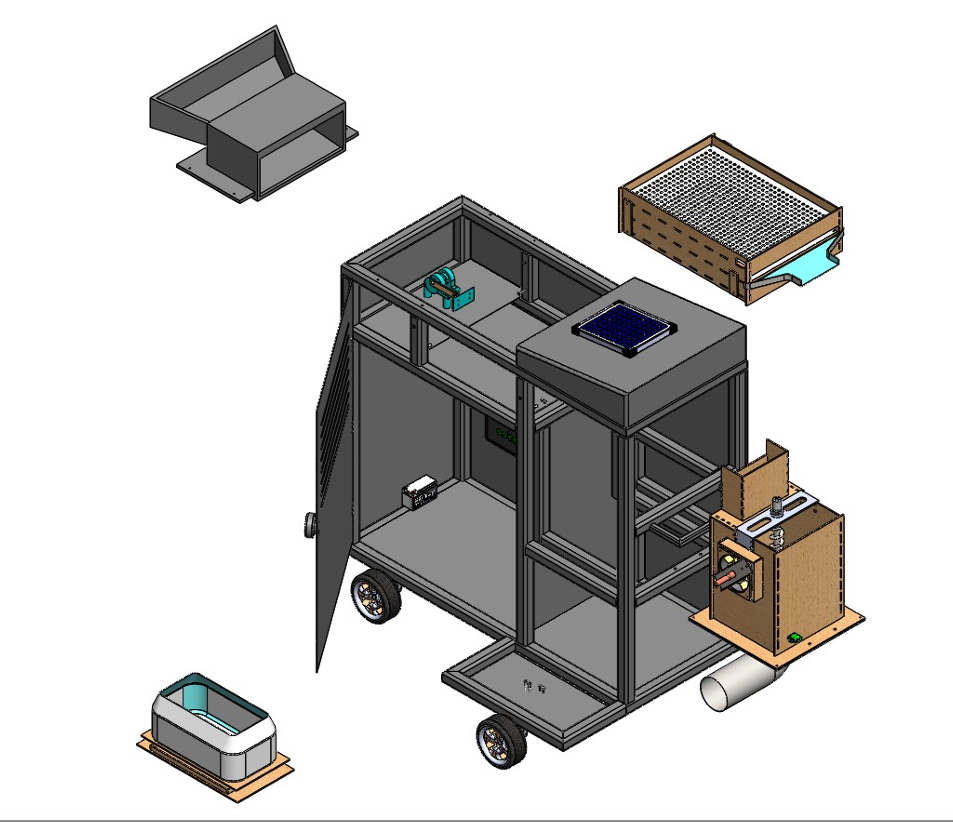
\includegraphics[width=0.85\textwidth]{images/Vue_modulaire_3D.PNG}
    \caption{Architecture modulaire du système SMART-SOJA — Vue d'ensemble CAO}
    \label{fig:cad_4blocs}
\end{figure}
\FloatBarrier


\begin{enumerate}
    \item \textbf{Bloc 1 — Unité d'entrée (Trémie) :} Trémie pyramidale à écoulement gravitaire, pilotée par le servomoteur SG90. Le capteur IR1 confirme la présence de soja avant l'ouverture.

    \item \textbf{Bloc 2 — Unité de nettoyage et vibration :} Deux tamis inox superposés montés sur suspensions élastiques. Le moteur JGA25-370 génère les oscillations via un système poulie-tige de transmission, assurant la séparation granulométrique.

    \item \textbf{Bloc 3 — Unité de séchage et analyse (Figure \ref{fig:sechage_pesee_cad}) :}
    \begin{itemize}
        \item \textbf{Vis sans fin} (type Archimède) : brassage mécanique continu pour un séchage homogène.
        \item \textbf{Ensemble Ventilateur + Résistance Chauffante} : circulation d'air chaud.
        \item \textbf{Boîtiers capteurs} : logements dédiés aux deux sondes capacitives (Soil1/Soil2) et au DHT22.
    \end{itemize}

    \begin{figure}[H]
        \centering
        \begin{subfigure}[b]{0.48\textwidth}
            \centering
            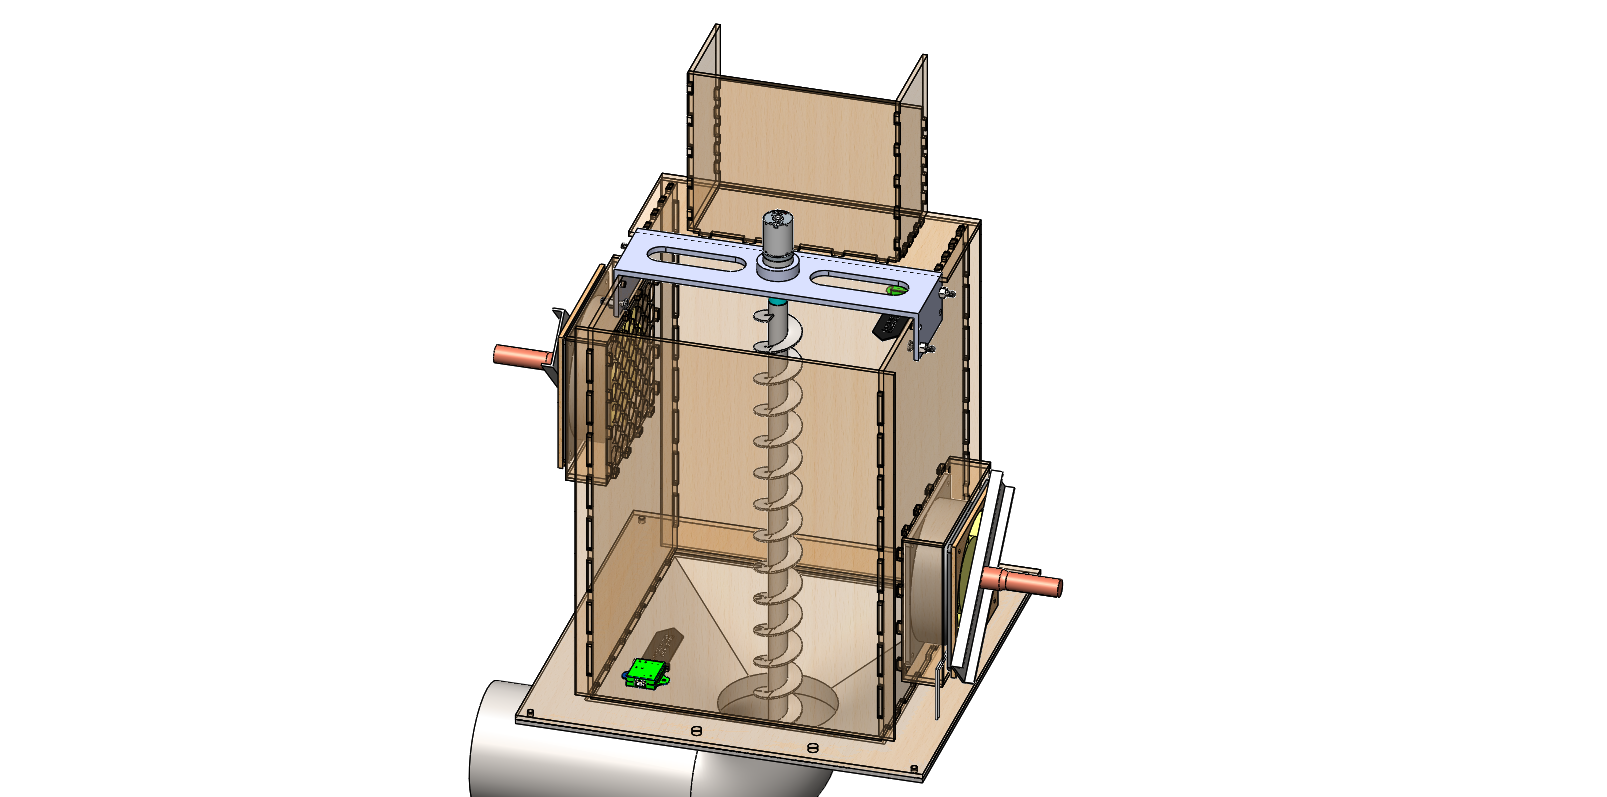
\includegraphics[width=\textwidth]{images/systeme_sechage.PNG}
            \caption{Unité de séchage (Vue 3D)}
        \end{subfigure}
        \hfill
        \begin{subfigure}[b]{0.48\textwidth}
            \centering
            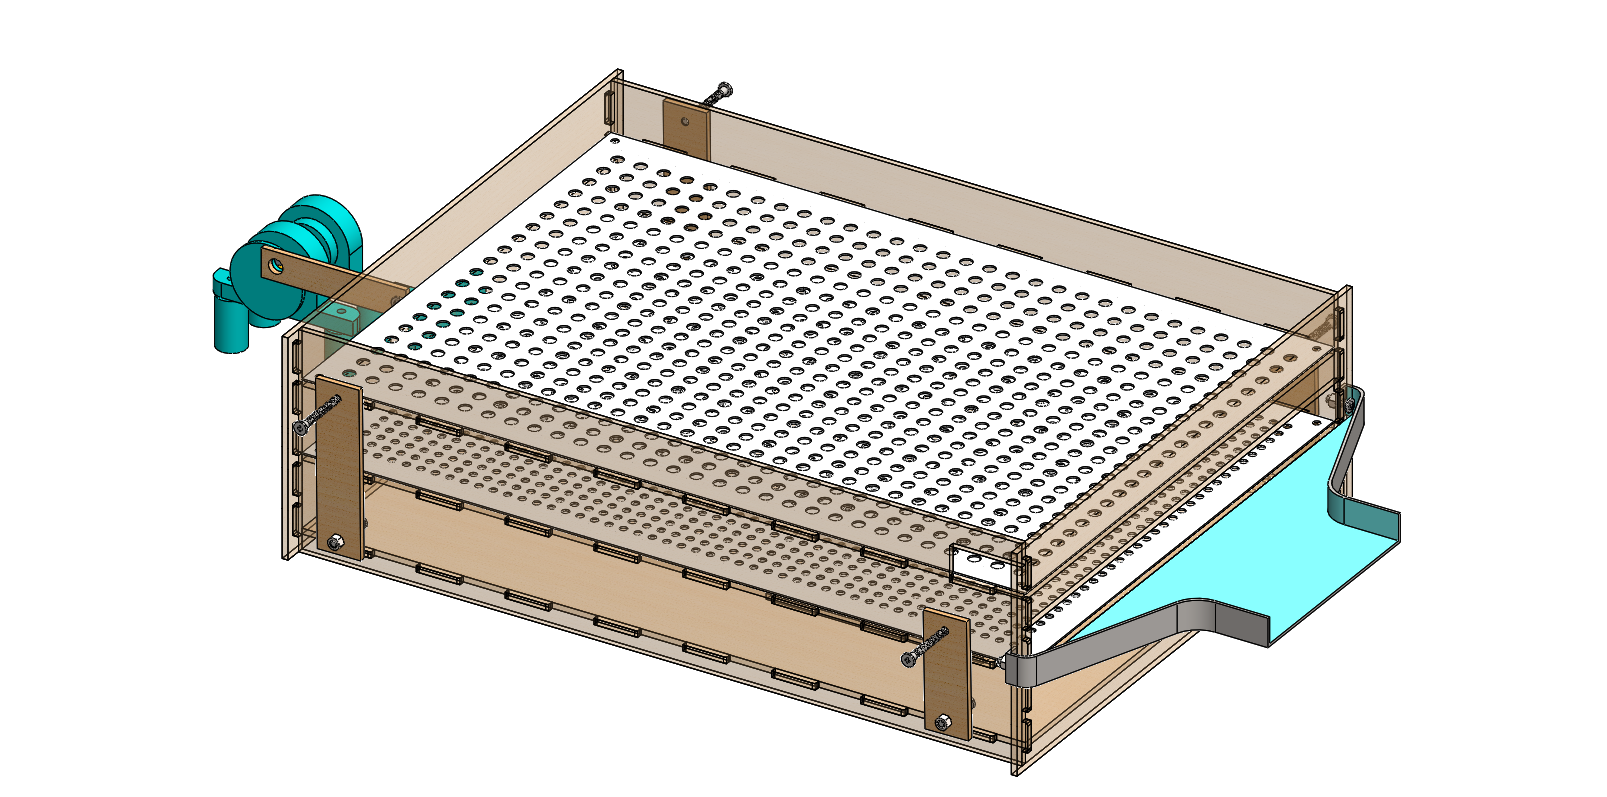
\includegraphics[width=\textwidth]{images/systeme_tami.PNG}
            \caption{Unité de tamisage (Vue 3D)}
        \end{subfigure}
        \caption{Détails des blocs de traitement mécanique sous SolidWorks}
        \label{fig:sechage_pesee_cad}
    \end{figure}
    \FloatBarrier


    \item \textbf{Bloc 4 — Unité de pesée et réception :} Support cellule de charge (Load Cell HX711) avec plateau de réception finale. Le capteur IR2 confirme le retrait du sac en fin de cycle.
\end{enumerate}

\begin{figure}[H]
    \centering
    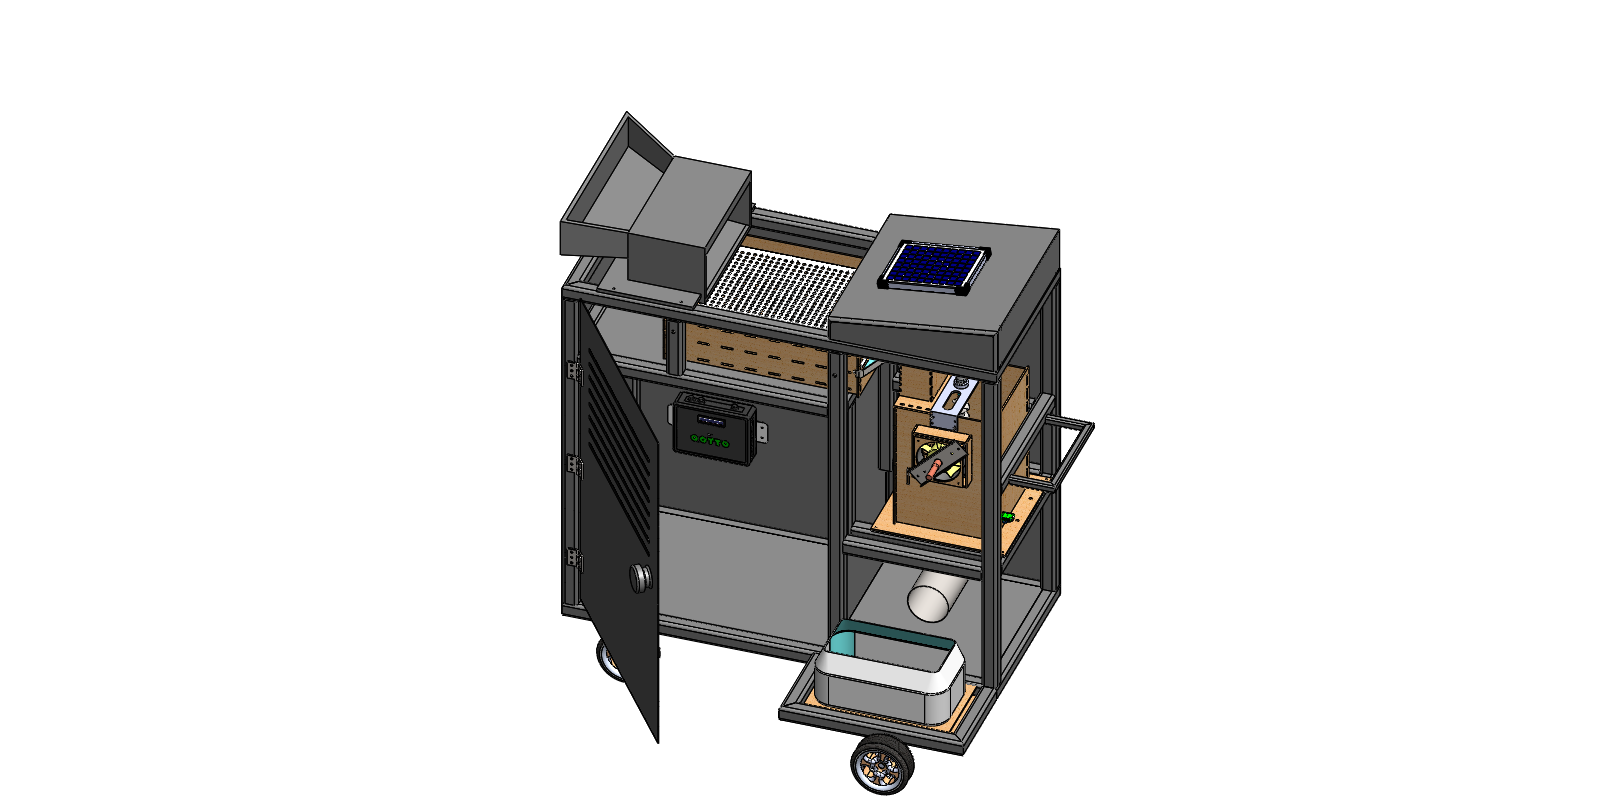
\includegraphics[width=1.02\textwidth]{images/Smart-Soja.PNG}
    \caption{Vue d'ensemble du prototype SMART-SOJA assemblé (SolidWorks)}
    \label{fig:systeme_complet}
\end{figure}
\FloatBarrier

\begin{figure}[H]
    \centering
    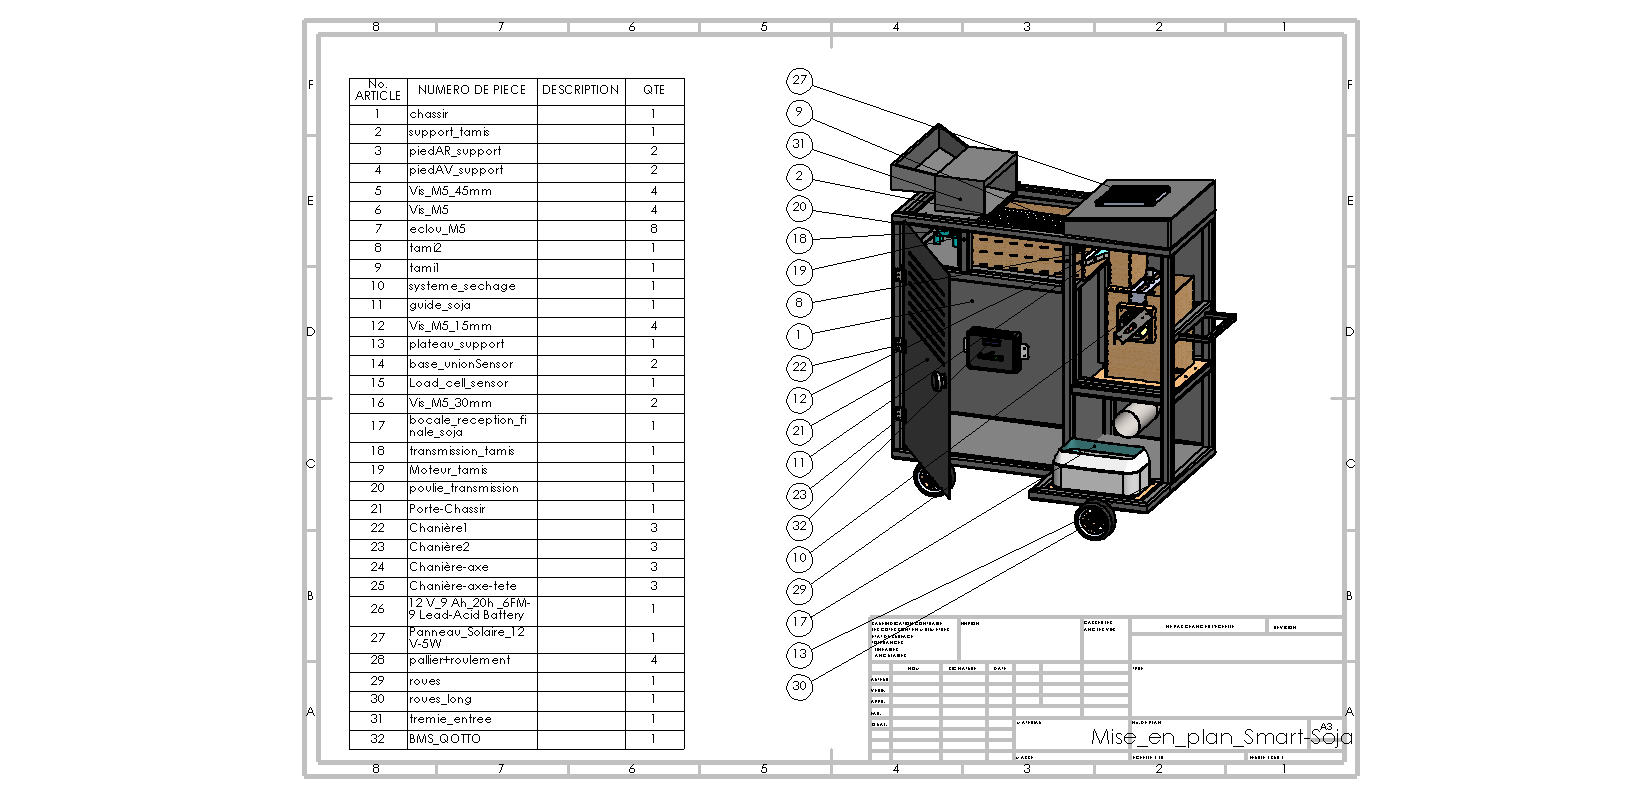
\includegraphics[width=\textwidth]{images/Mise_en_plan_Smart-Soja.PNG}
    \caption{Mise en plan technique et nomenclature (BOM) du châssis}
    \label{fig:mise_en_plan}
\end{figure}
\FloatBarrier

Chaque bloc peut être retiré du châssis sans démonter l'intégralité du système grâce à un système de glissières et connecteurs rapides — facteur clé pour la maintenance en milieu rural isolé.

\subsection{Fabrication et assemblage physique du châssis}
La phase de fabrication mécanique du châssis a nécessité la découpe de panneaux de contreplaqué haute densité aux dimensions précises de la modélisation SolidWorks. Cette opération a été réalisée à l'atelier de \textbf{Sèmè City Open Park} à l'aide d'une scie circulaire sur table (Figure~\ref{fig:decoupe_contreplaque}).

\begin{figure}[H]
    \centering
    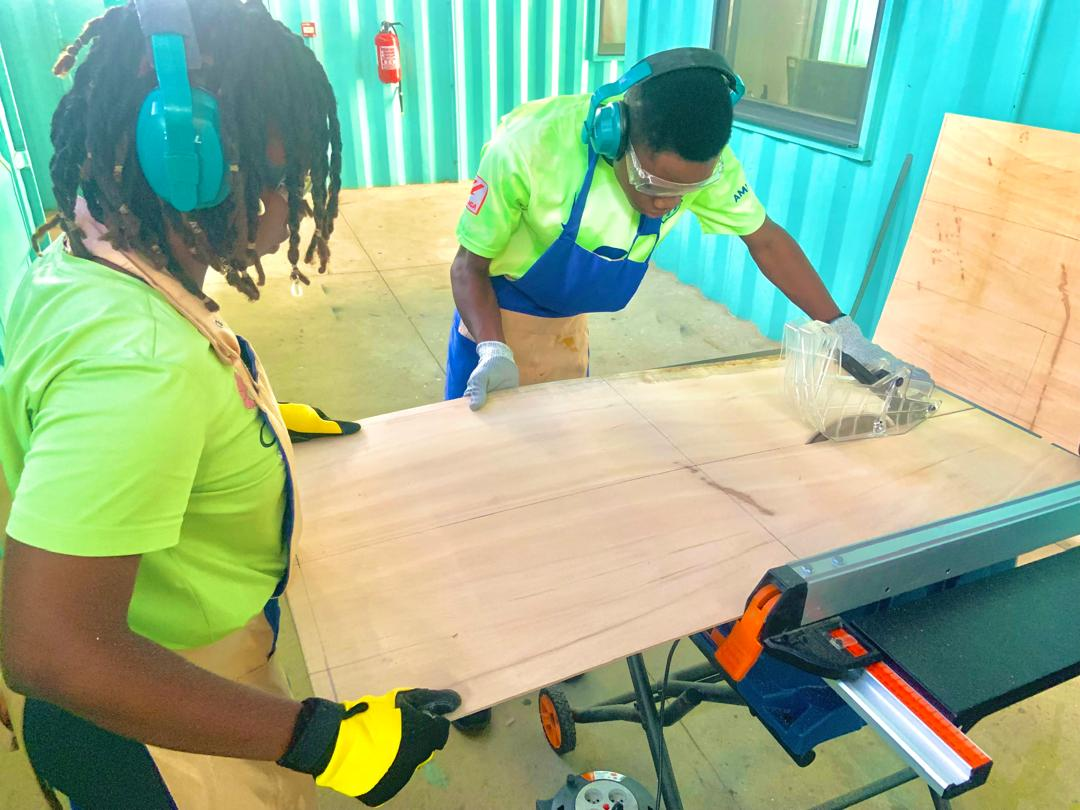
\includegraphics[width=0.55\textwidth]{images/decoupe_plaquet.jpg}
    \caption{Découpe du contreplaqué pour le châssis SMART-SOJA à Sèmè City Open Park}
    \label{fig:decoupe_contreplaque}
\end{figure}
\FloatBarrier

% -------------------------------------------------------
\section{Implémentation du firmware embarqué}
% -------------------------------------------------------
\label{sec:freertos_implementation}

\subsection{Architecture multitâches FreeRTOS}
Le firmware SMART-SOJA implémente \textbf{6 tâches FreeRTOS} ordonnancées selon leur criticité. La communication inter-tâches s'effectue via 5 files de messages (queues) pour un découplage robuste sans conditions de course (Tableau \ref{tab:freertos_tasks}).

\begin{table}[H]
    \caption{Hiérarchie des tâches FreeRTOS du firmware SMART-SOJA}
    \label{tab:freertos_tasks}
    \centering
    \small
    \renewcommand{\arraystretch}{1.8}
    \rowcolors{2}{white}{lightGray}
    \begin{tabularx}{\textwidth}{|L|>{\bfseries}C|C|L|}
        \hline
        \rowcolor{lightGray}
        \textbf{Tâche} & \textbf{Priorité} & \textbf{Cycle} & \textbf{Fonction} \\ \hline
        Task\_Safety    & 4 (MAX)  & 10 ms  & Arrêt d'urgence, surchauffe, timeout — temps réponse $<$ 10 ms. \\ \hline
        Task\_Control   & 3 (HIGH) & 50 ms  & Automate GRAFCET, gestion des transitions d'états. \\ \hline
        Task\_Sensing   & 2 (MED)  & 100 ms & Acquisition DHT22, Soil1/2, HX711 avec filtrage passe-bas. \\ \hline
        Task\_Actuators & 2 (MED)  & 50 ms  & Pilotage PWM moteurs, servo, LEDs. \\ \hline
        Task\_LCD       & 1 (LOW)  & 200 ms & Affichage I2C + lecture potentiomètres (ADC 0--4095 → 0--100\%). \\ \hline
        Task\_MQTT      & 1 (LOW)  & 500 ms & Transmission JSON, Store-and-Forward sur SD si déconnecté. \\ \hline
    \end{tabularx}
\end{table}
\FloatBarrier

Le flux de synchronisation entre tâches est illustré en Figure \ref{fig:arch_freertos} :

\begin{figure}[H]
    \centering
    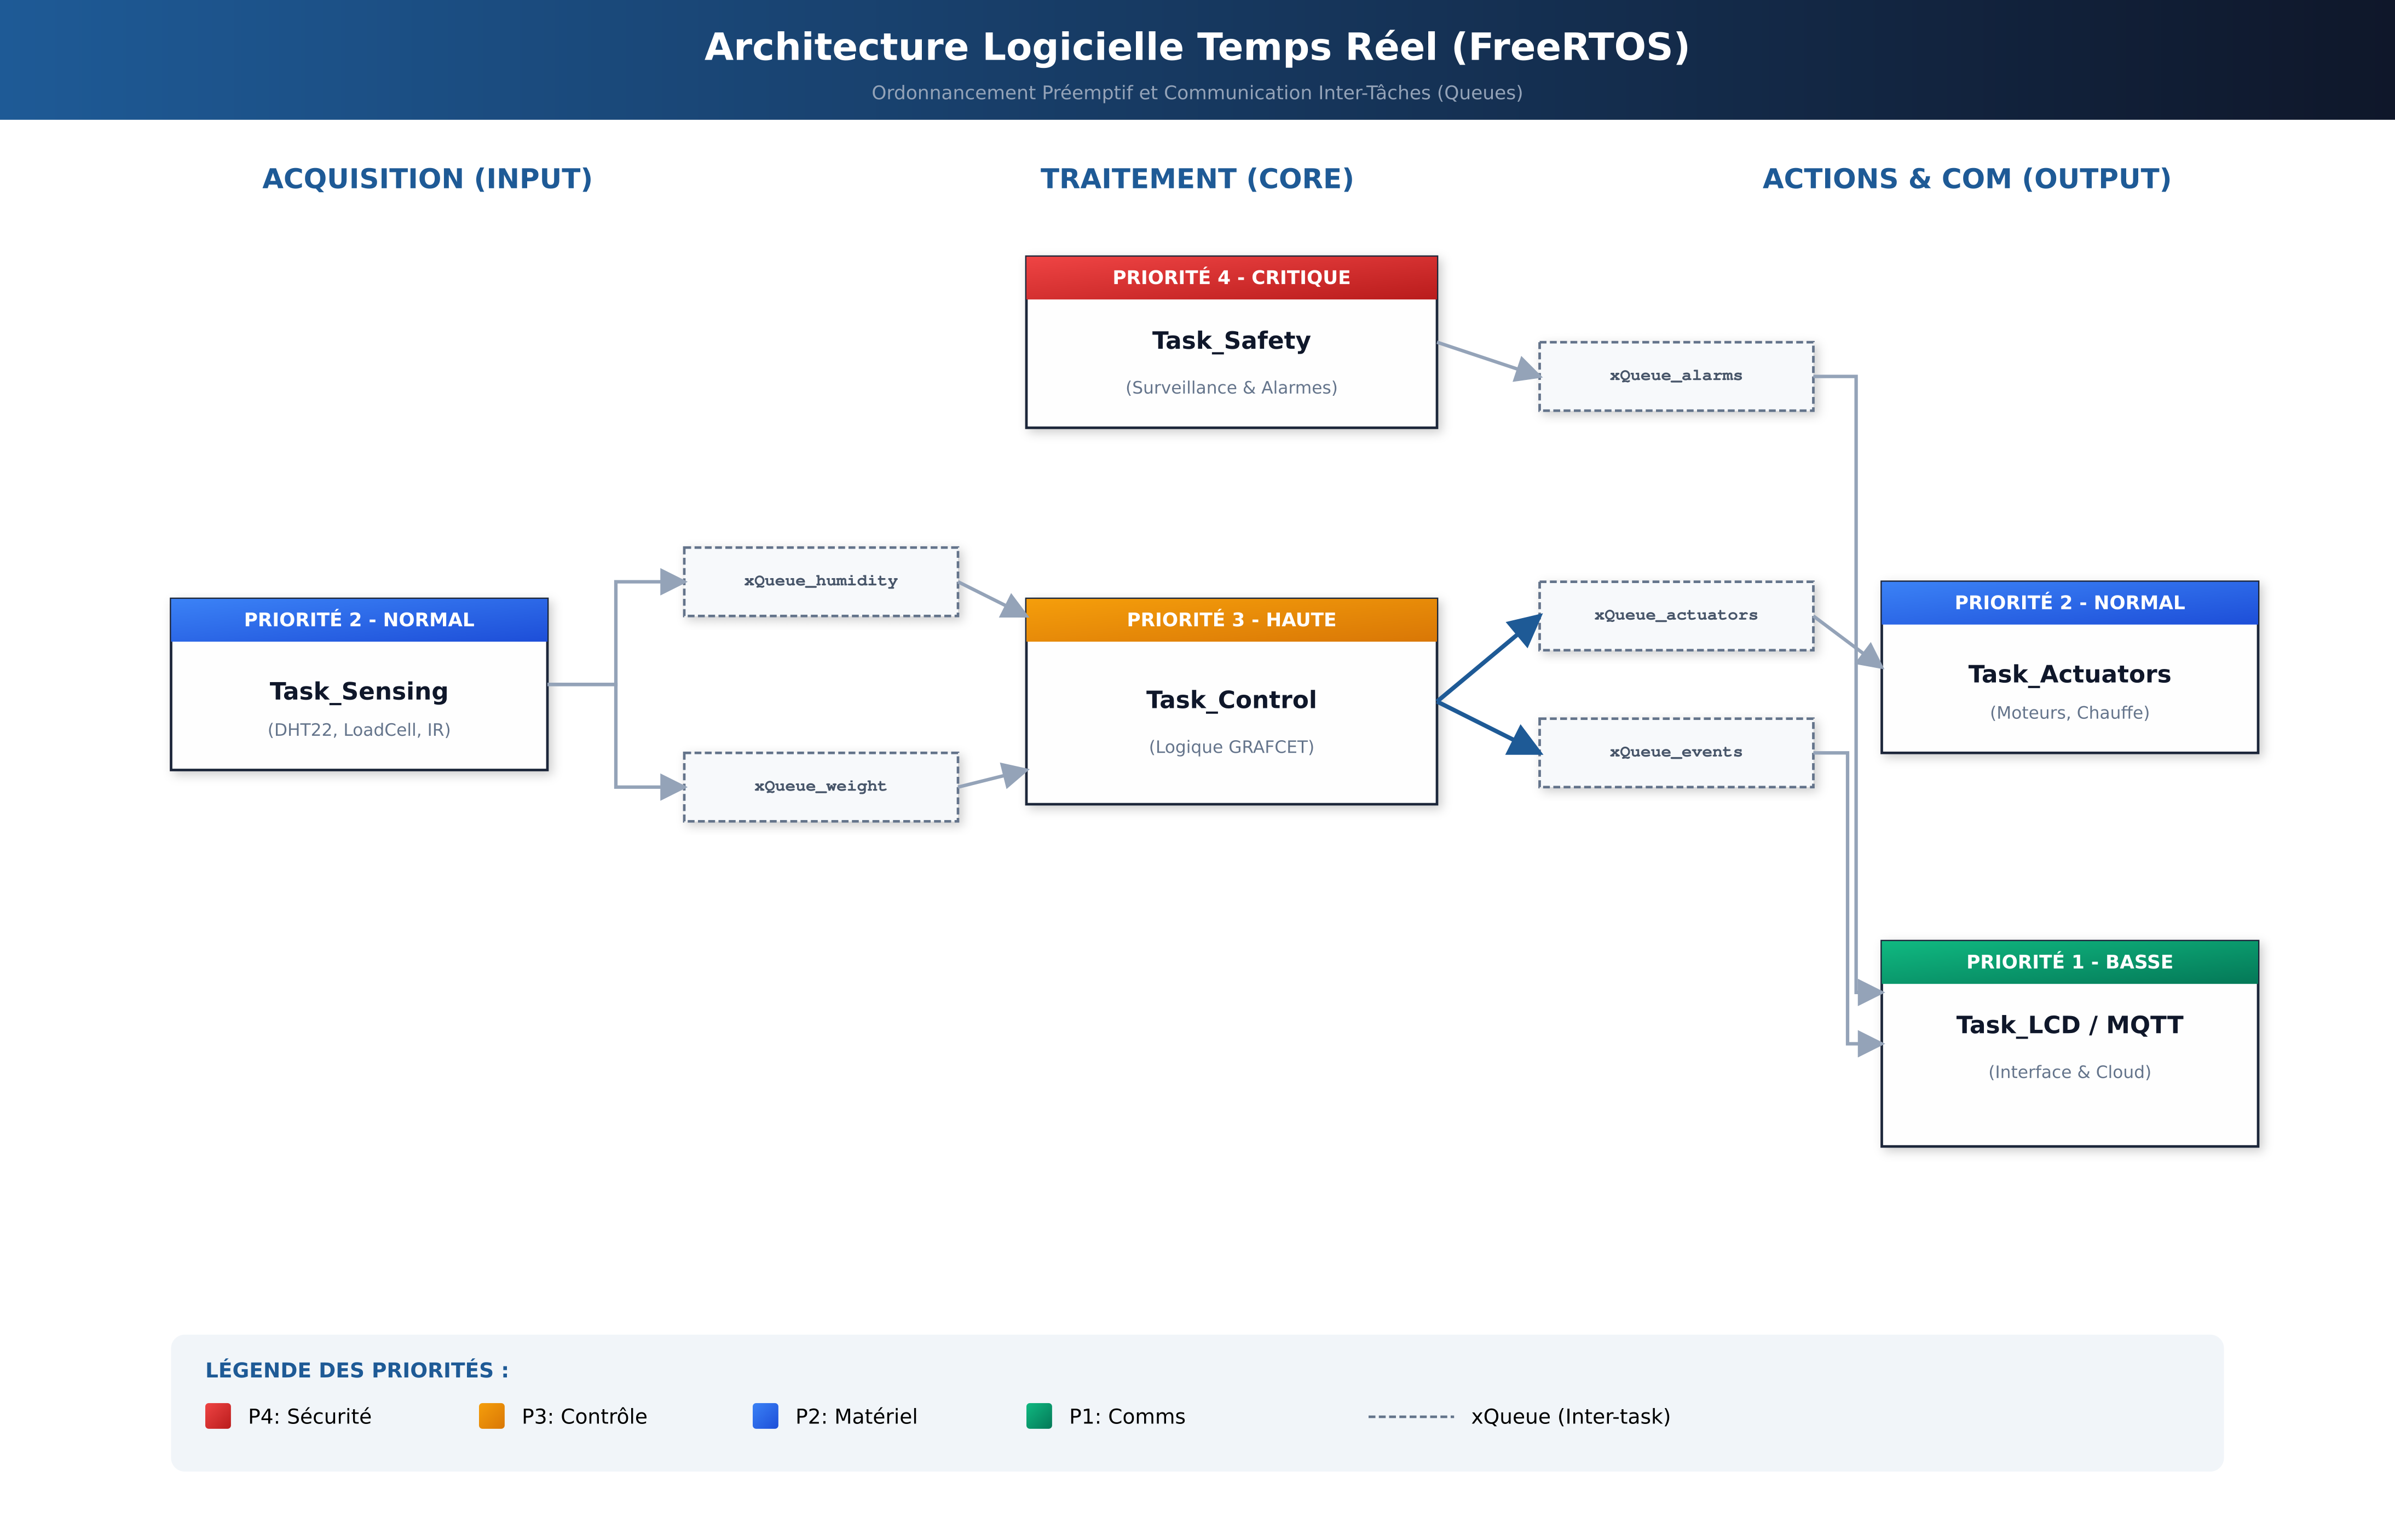
\includegraphics[width=\textwidth]{images/freertos_tasks.png}
    \caption{Diagramme de synchronisation des tâches FreeRTOS — SMART-SOJA}
    \label{fig:arch_freertos}
\end{figure}
\FloatBarrier

\subsection{Sérialisation et format de données (JSON)}
L'échange de données entre l'unité mobile ESP32 et la plateforme web de supervision s'effectue sous forme de messages sérialisés au format JSON. Deux types de trames sont principalement transmis :

\vspace{0.3cm}
\noindent\textbf{1. Trame de télémétrie périodique} (publiée toutes les 5~secondes sur le topic \texttt{smart-soja/telemetry/\{unitId\}}) : elle assure le suivi en temps réel de l'état de fonctionnement du prototype.
\begin{verbatim}
{
  "unitId": "SS-000110",
  "timestamp": 1716633600000,
  "humidity": 12.5,
  "temperature": 31.8,
  "weight": 42.3,
  "ir1": true,
  "ir2": false,
  "mode": "auto",
  "step": 3,
  "alarm": false,
  "controls": {
    "alimentation": false,
    "tamis": true,
    "ventilateur": false,
    "chauffage": true,
    "vis_soja": true,
    "servo_vanne": false
  },
  "battery": 95
}
\end{verbatim}

\vspace{0.3cm}
\noindent\textbf{2. Trame d'archivage de fin de cycle} (publiée sur le topic \texttt{smart-soja/lot\_completed/\{unitId\}} lors de la finalisation du traitement d'un lot) : elle certifie la qualité finale du soja.
\begin{verbatim}
{
  "unitId": "SS-000110",
  "timestamp": 1716633780000,
  "lotId": "LOT-TEST-002",
  "duration_ms": 180000,
  "weight_processed": 5000,
  "humidity_avg": 10.8,
  "temperature_avg": 31.8,
  "steps_completed": 12,
  "quality_score": 95
}
\end{verbatim}
\vspace{0.2cm}

Ce format de \textbf{passeport numérique} constitue la pièce centrale de la traçabilité Internet des objets : il lie chaque sac de soja à ses métriques de qualité certifiées, consultables depuis le tableau de bord web.

% -------------------------------------------------------
\section{Plateforme Internet des objets : tableau de bord de supervision}
% -------------------------------------------------------
La plateforme web \textbf{SMART-SOJA} constitue le centre de supervision et de traçabilité à distance du système. Elle a été développée selon une architecture de type \textbf{SPA} (\textit{Single Page Application}) en utilisant l'outillage moderne \textbf{Vite.js} et du \textbf{JavaScript (Vanilla JS)}. Ce choix garantit une interface utilisateur fluide, réactive et optimisée pour une consultation sur terminaux mobiles comme sur ordinateurs.

Le flux de données (Figure \ref{fig:diagram_mqtt}) repose sur un pipeline de communication bidirectionnel :
\begin{enumerate}
    \item \textbf{Collecte et Transport :} L'unité mobile publie les données de chaque lot au format JSON via le protocole \textbf{MQTT}.
    \item \textbf{Passerelle et Persistance :} Un serveur bridge sous \textbf{Node.js} intercepte ces messages pour les valider et les enregistrer instantanément dans la base de données temps réel \textbf{Firebase (Firestore)}.
    \item \textbf{Visualisation :} La plateforme web se synchronise automatiquement avec Firebase, permettant aux utilisateurs de suivre l'évolution de l'humidité et du poids des grains sans avoir à rafraîchir la page.
\end{enumerate}

\begin{figure}[H]
    \centering
    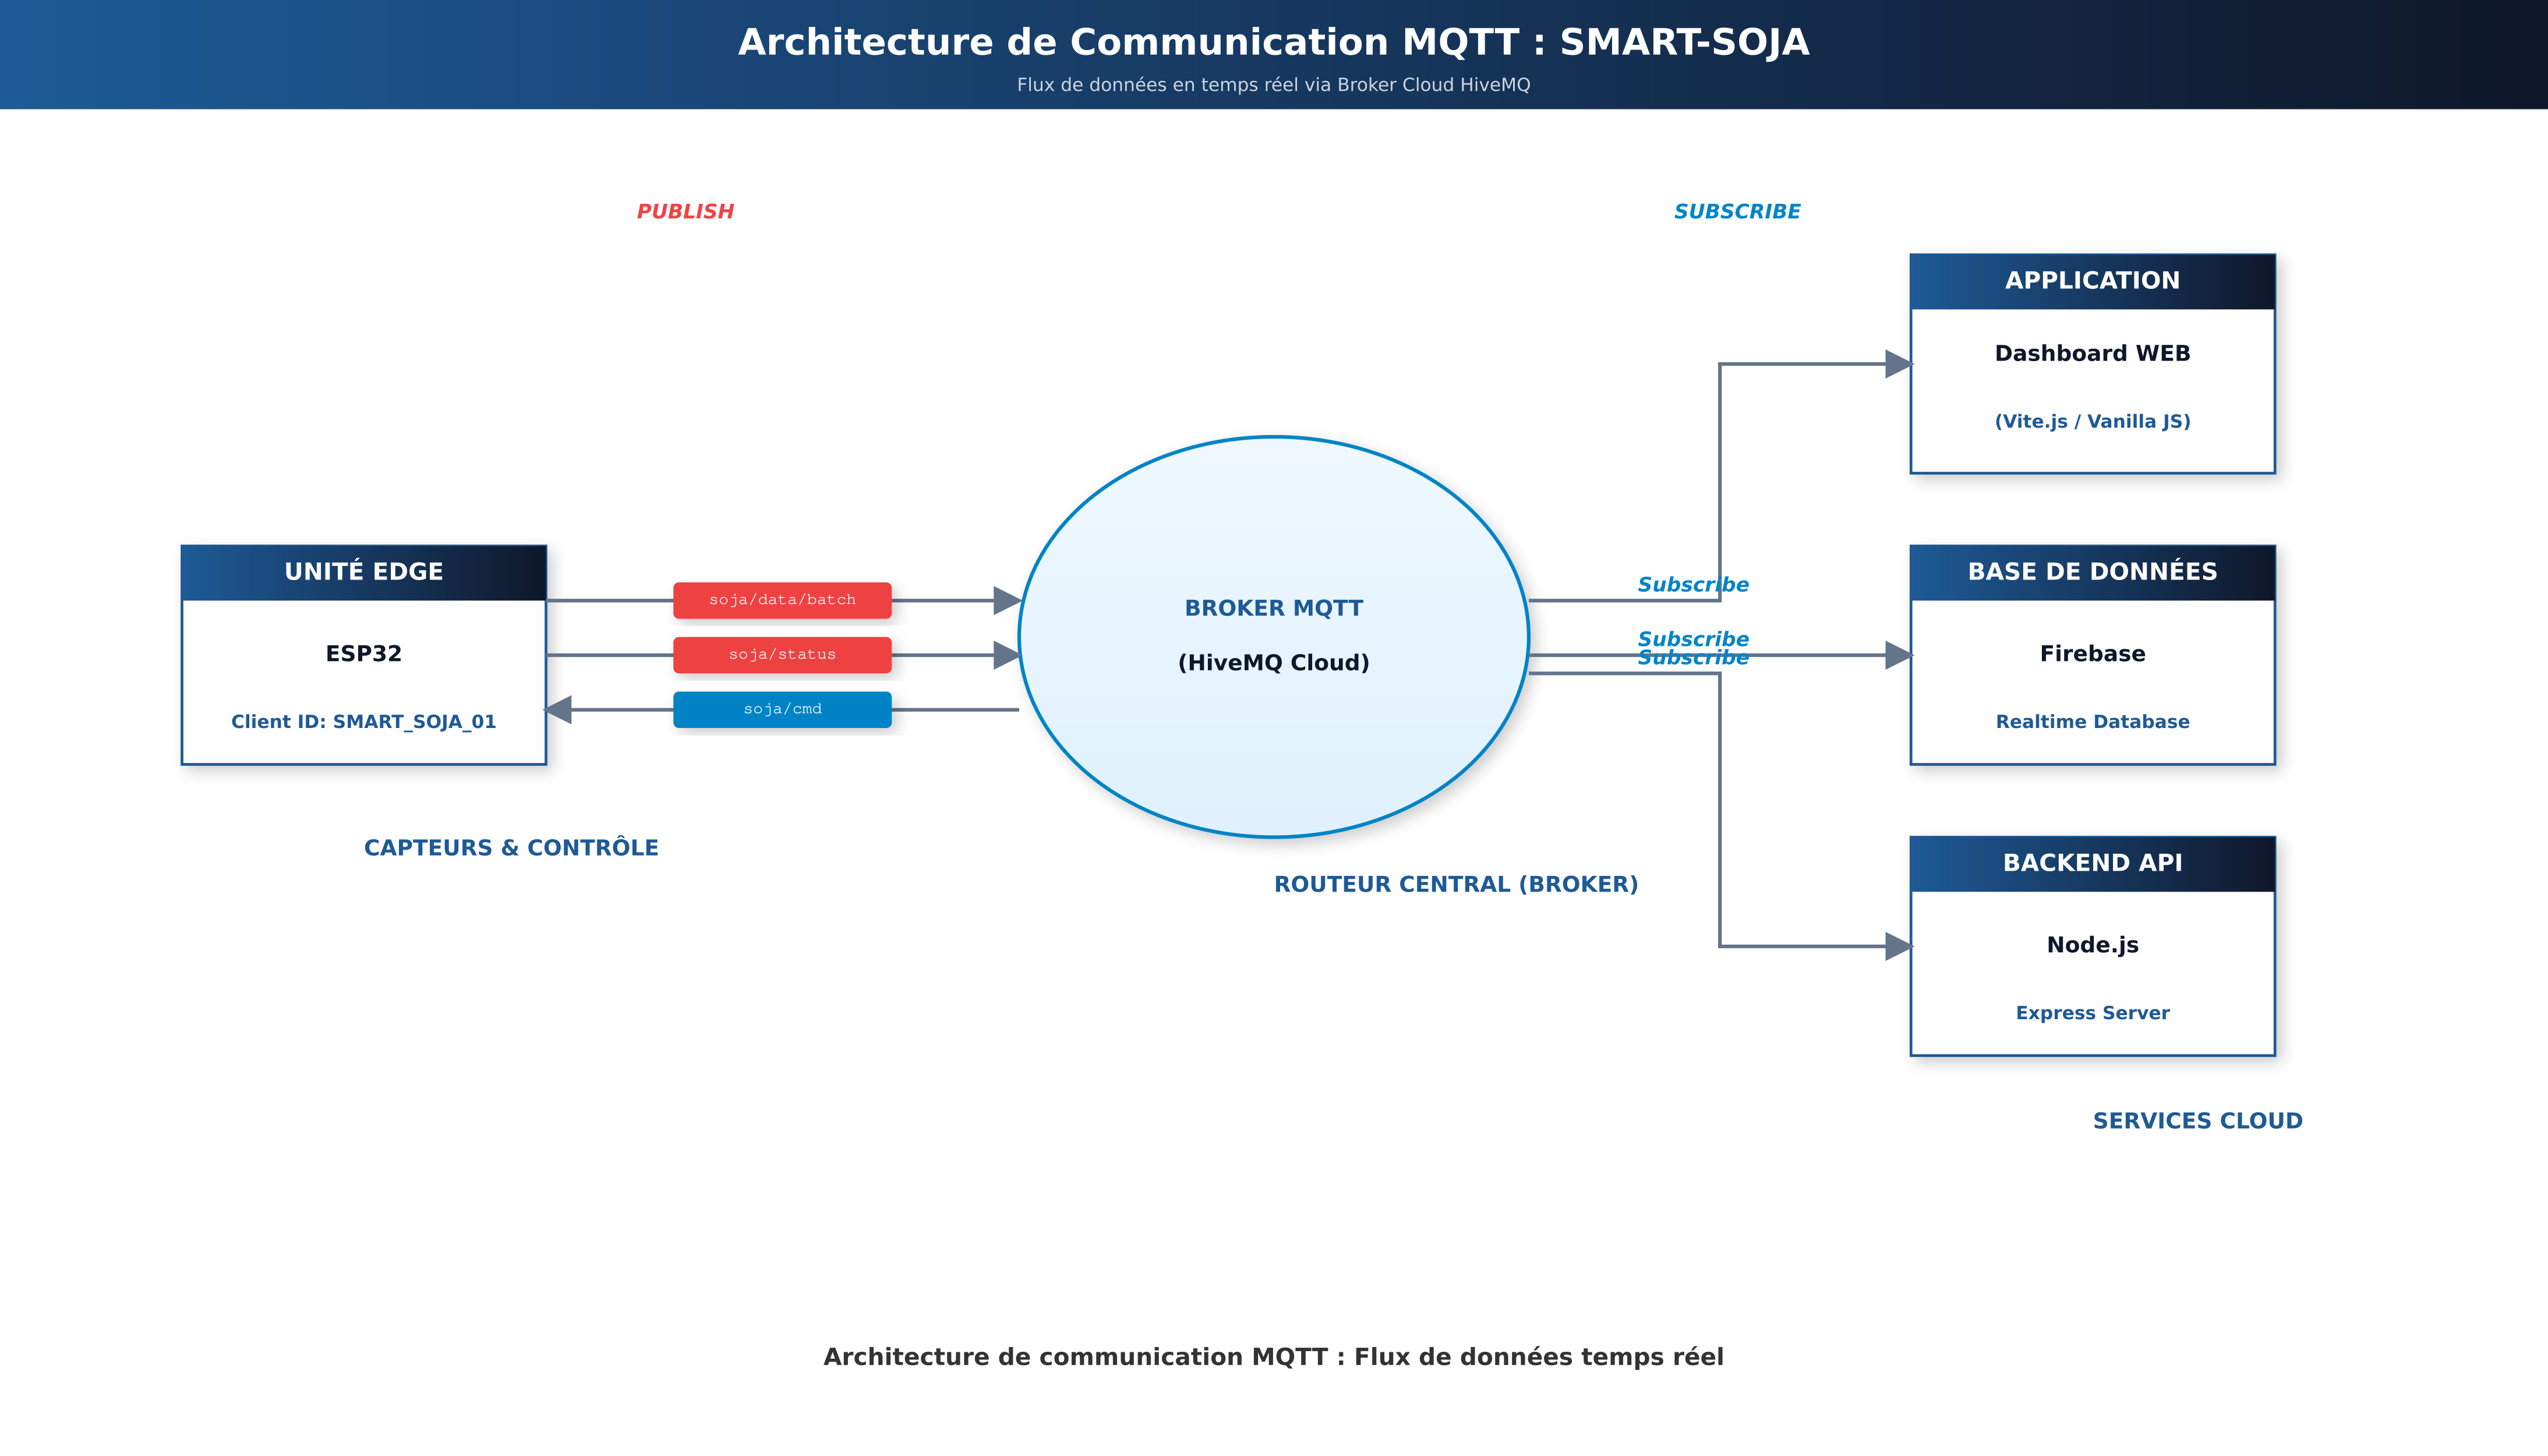
\includegraphics[width=\textwidth]{images/mqtt_architecture.png}
    \caption{Architecture de communication MQTT : Pipeline de données temps réel}
    \label{fig:diagram_mqtt}
\end{figure}
\FloatBarrier

Cette architecture garantit une \textbf{intégrité totale de la traçabilité} : chaque sac de soja possède son propre passeport numérique stocké de manière sécurisée dans le Cloud.

\begin{figure}[H]
    \centering
    \begin{subfigure}[b]{0.48\textwidth}
        \centering
        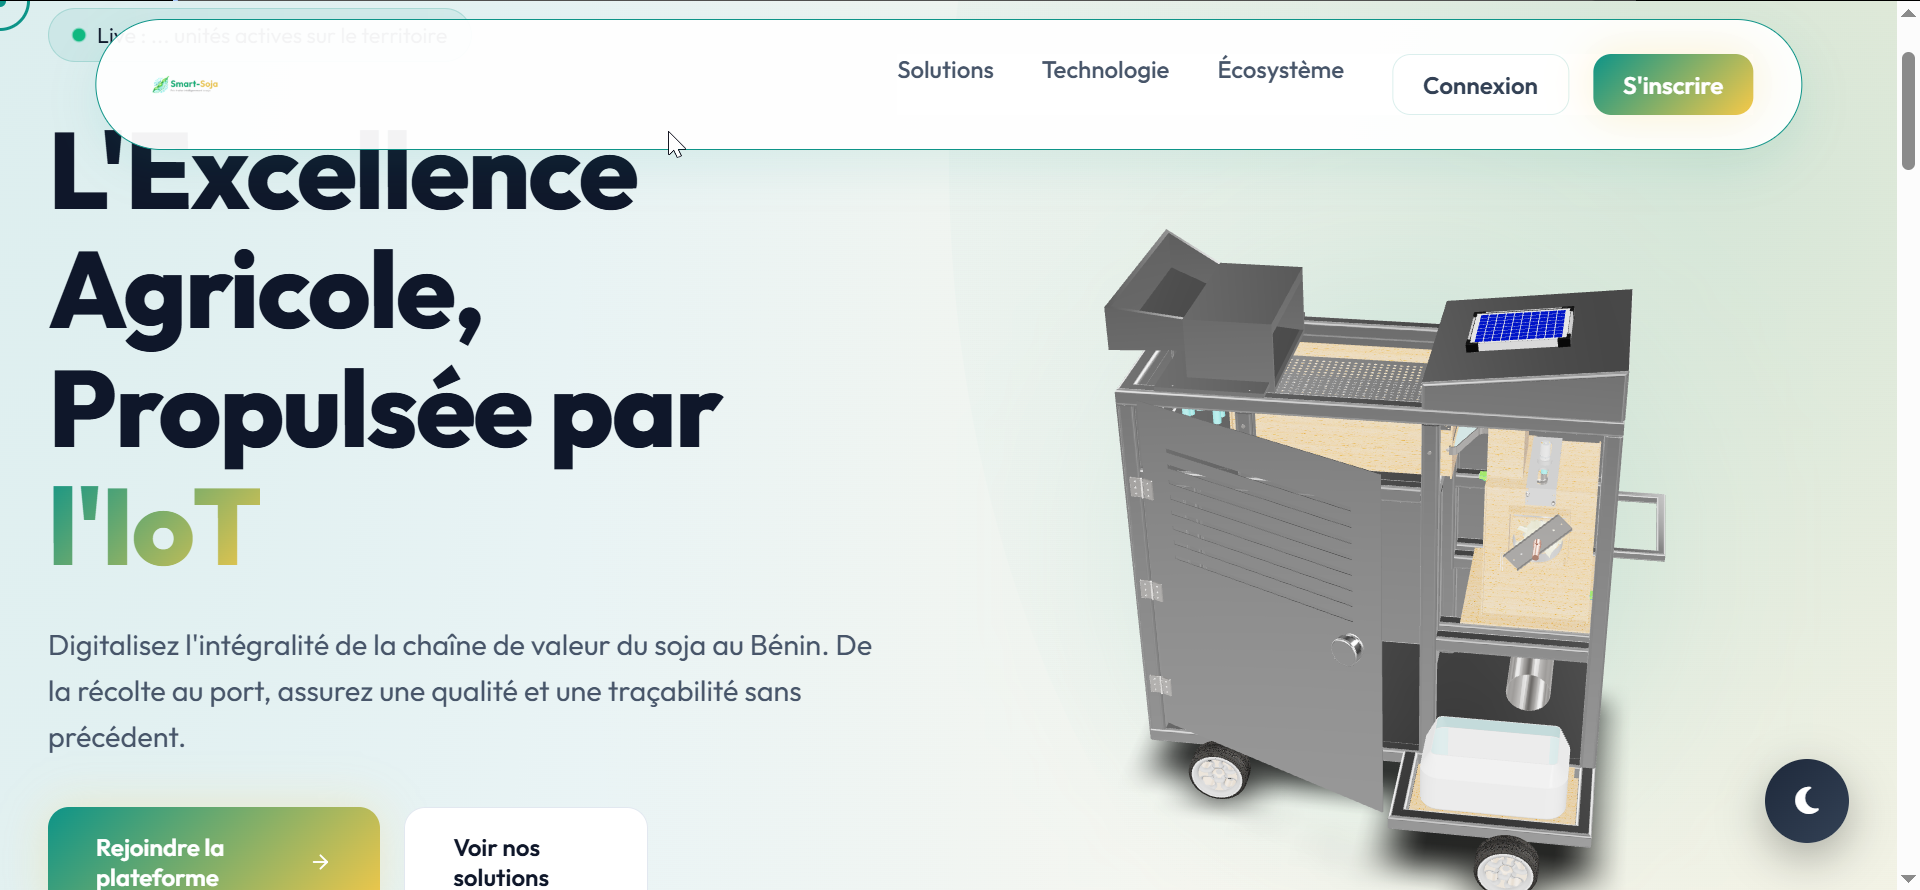
\includegraphics[width=\textwidth]{images/smart-soja-web_light.png}
        \caption{Mode Clair (\textit{Light Theme})}
    \end{subfigure}
    \hfill
    \begin{subfigure}[b]{0.48\textwidth}
        \centering
        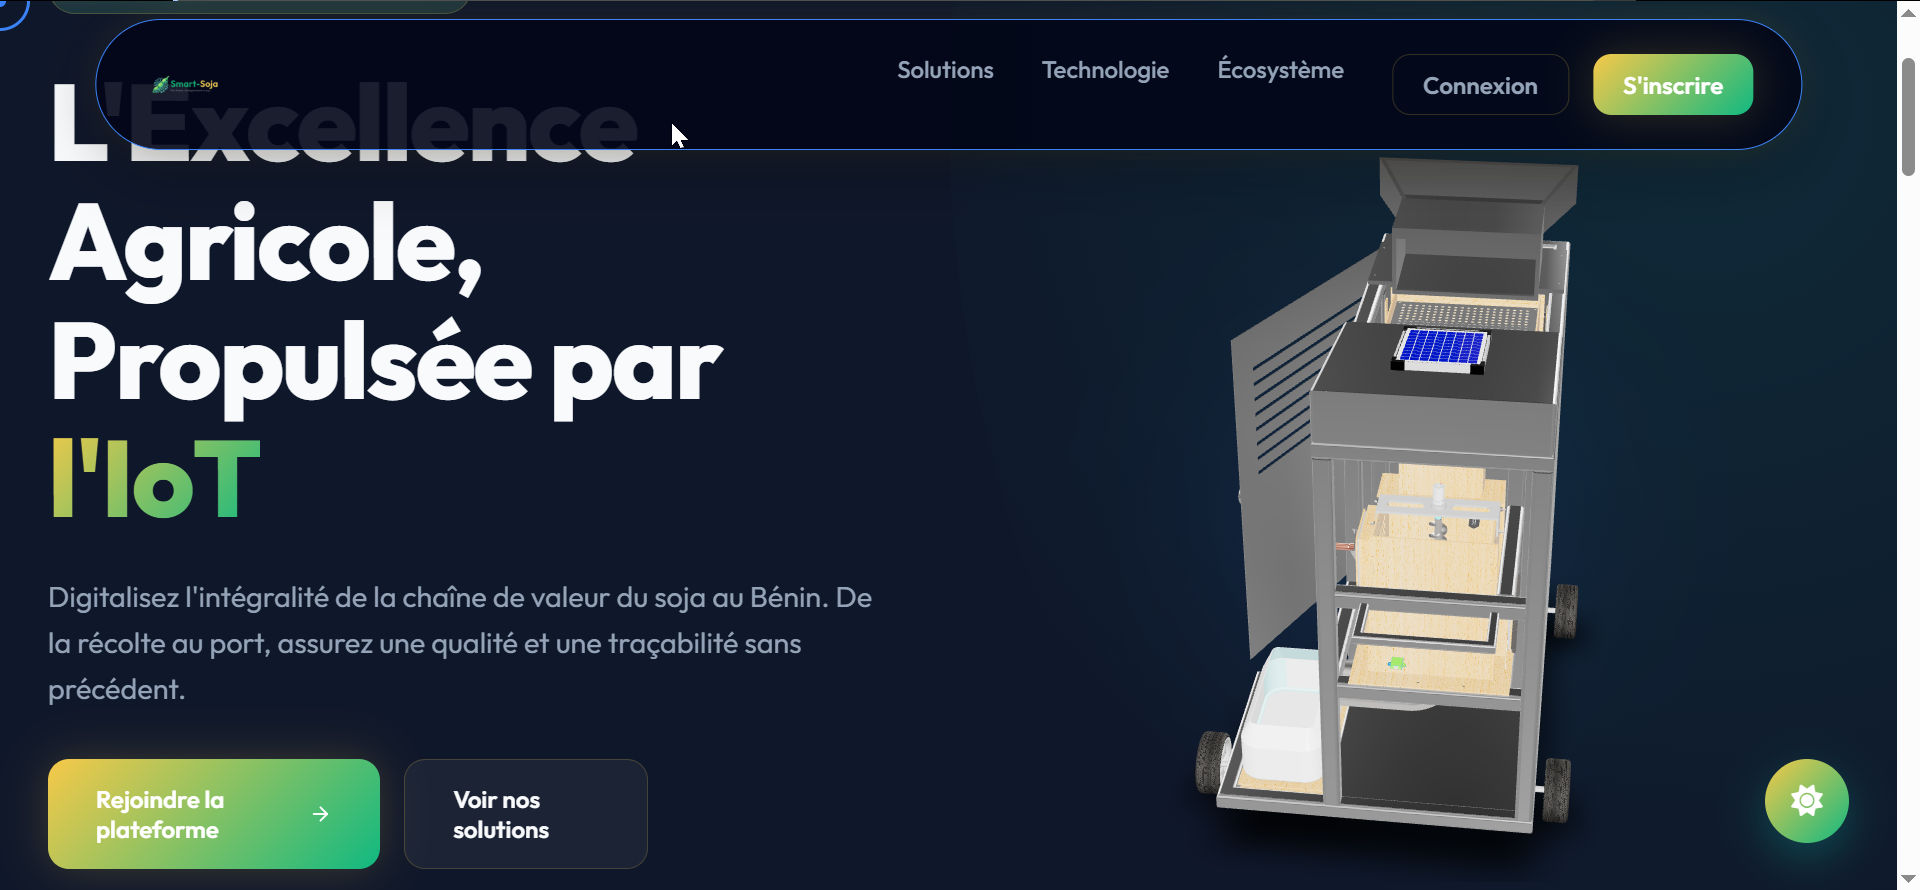
\includegraphics[width=\textwidth]{images/smart-soja-web_dark.png}
        \caption{Mode Sombre (\textit{Dark Theme})}
    \end{subfigure}
    \caption{Interface de présentation du projet SMART-SOJA — Page d'accueil (Vues multi-thèmes)}
    \label{fig:dashboard_themes}
\end{figure}
\FloatBarrier

Trois profils d'accès sont proposés :
\begin{itemize}
    \item \textbf{Tableau de bord Exploitant :} Suivi de production en temps réel, contrôle manuel des actionneurs via MQTT, alertes de maintenance.
    \item \textbf{Tableau de bord Industrie (GDIZ Ready) :} Validation de la qualité des lots entrants, graphiques d'humidité et température, impression des certificats de traçabilité PDF.
    \item \textbf{Tableau de bord Admin :} Gestion de la flotte de machines et des utilisateurs, audit système.
\end{itemize}

\FloatBarrier

% Fin de la section conception


\section*{Synthèse et transition}
Ce chapitre a présenté l'ensemble de la démarche de conception du système SMART-SOJA, depuis l'analyse du contexte de la filière soja au Bénin jusqu'à la réalisation concrète du prototype. L'architecture modulaire retenue, combinant mécanique, électronique, informatique embarquée et connectivité IoT, aboutit à un système cohérent et fonctionnel. Afin de valider la viabilité de cette solution mécatronique et de vérifier sa conformité au cahier des charges fonctionnel sous des contraintes réelles, une série d'essais expérimentaux a été menée sur le site de QOTTO Bénin. Les résultats quantitatifs de cette phase d'évaluation des performances, ainsi que leur analyse critique et les discussions associées, font l'objet du chapitre suivant.
     % Chap 2 : Étude de la solution proposée
% ================== CHAPITRE 3 : RÉSULTATS, ANALYSE ET DISCUSSION ==================
\chapter{Résultats, analyse et discussion}
\label{chap:resultats}

Ce chapitre présente la validation fonctionnelle du prototype \textbf{SMART-SOJA}. À la phase actuelle d'assemblage et d'intégration (juin 2026), l'approche adoptée consiste à démontrer la faisabilité technique et la conformité des sous-systèmes individuels à travers des tests unitaires rigoureux, des mesures quantifiées et une démonstration de la chaîne numérique de traçabilité. Les résultats documentent l'état de validation technique atteint à ce stade du projet, en distinguant clairement les démonstrations fonctionnelles déjà réalisées des améliorations et validations complémentaires envisagées.

% -------------------------------------------------------
\section{Présentation du prototype physique réalisé}
% -------------------------------------------------------

Avant de détailler les résultats de la validation fonctionnelle, il convient de présenter le prototype physique de \textbf{SMART-SOJA} tel qu'il a été assemblé et intégré à ce stade d'avancement (juin 2026). Cette réalisation concrétise les modèles de conception assistée par ordinateur (CAO) 3D et les routages de cartes électroniques présentés au Chapitre 2.

Le système est structuré sous forme de blocs physiques distincts montés sur un châssis robuste en acier (tubes de 30×30~mm) et parois en contreplaqué, assurant à la fois la rigidité mécanique nécessaire pour supporter les vibrations du tamisage et l'isolation thermique requise pour le séchage.

La Figure~\ref{fig:realisation_blocs} présente les trois principaux sous-ensembles physiques de la machine :
\begin{itemize}
    \item \textbf{Le bloc d'entrée (Figure~\ref{fig:real_bloc_entree}) :} Il comprend la trémie d'alimentation supérieure, équipée d'un système de distribution en utilisant un servomoteur S90 et de capteurs infrarouges de détection de niveau pour réguler le débit de soja.
    \item \textbf{Le bloc de tamisage (Figure~\ref{fig:real_bloc_tamis}) :} Ce sous-système suspendu intègre le cadre du tamis vibrant, entraîné par un moteur DC pour séparer les impuretés du soja par granulométrie et tamisage mécanique.
    \item \textbf{Le bloc de séchage actif (Figure~\ref{fig:real_bloc_sechage}) :} Il abrite la chambre de séchage équipée des résistances chauffantes alimentées en 12~V DC, d'un ventilateur pour homogénéiser l'air chaud, de sondes capacitives intégrées pour le suivi de l'humidité en cours de traitement et d'une vis sans fin commandée par un moteur DC pour faciliter le brassage du soja.
\end{itemize}

\begin{figure}[H]
    \centering
    \begin{subfigure}[b]{0.32\textwidth}
        \centering
        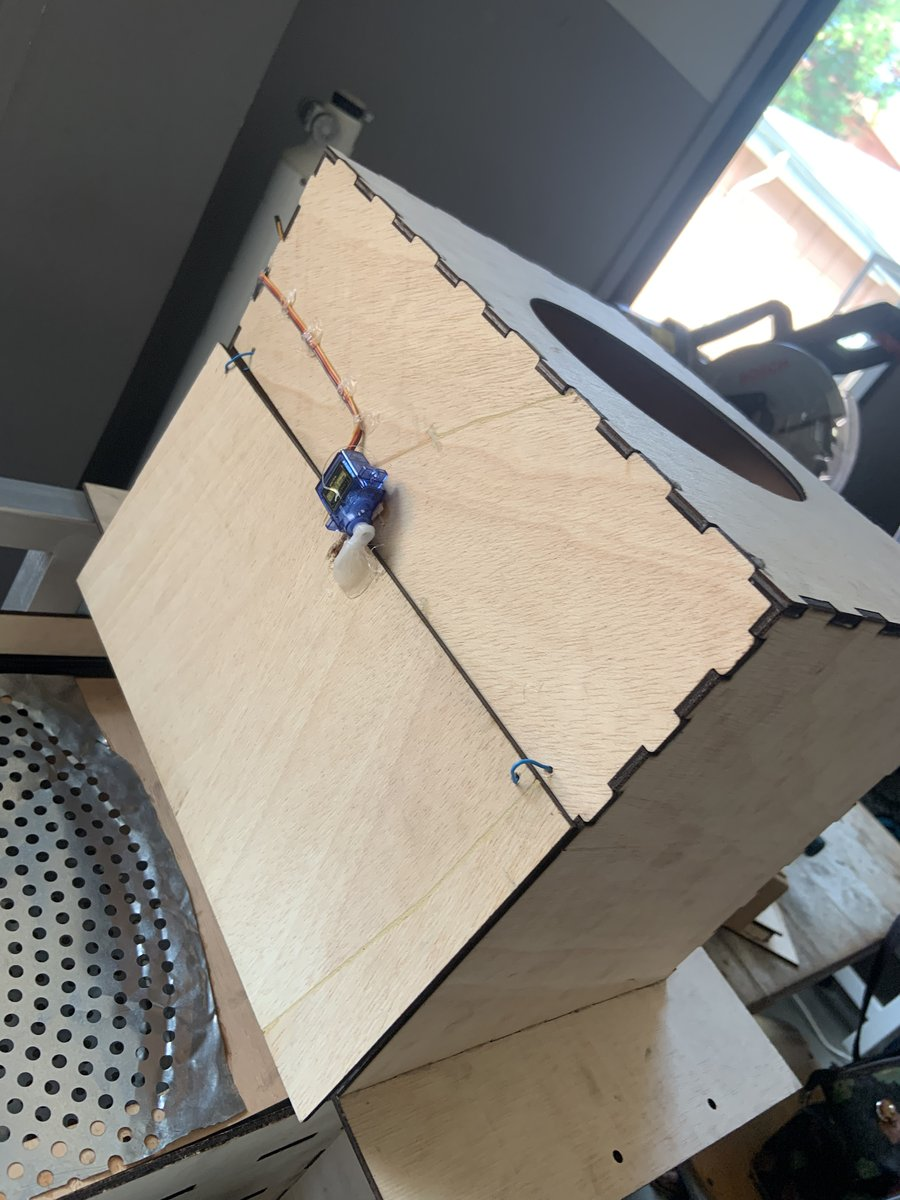
\includegraphics[width=\textwidth]{images/image_bloc_entree.jpg}
        \caption{Bloc d'alimentation}
        \label{fig:real_bloc_entree}
    \end{subfigure}
    \hfill
    \begin{subfigure}[b]{0.32\textwidth}
        \centering
        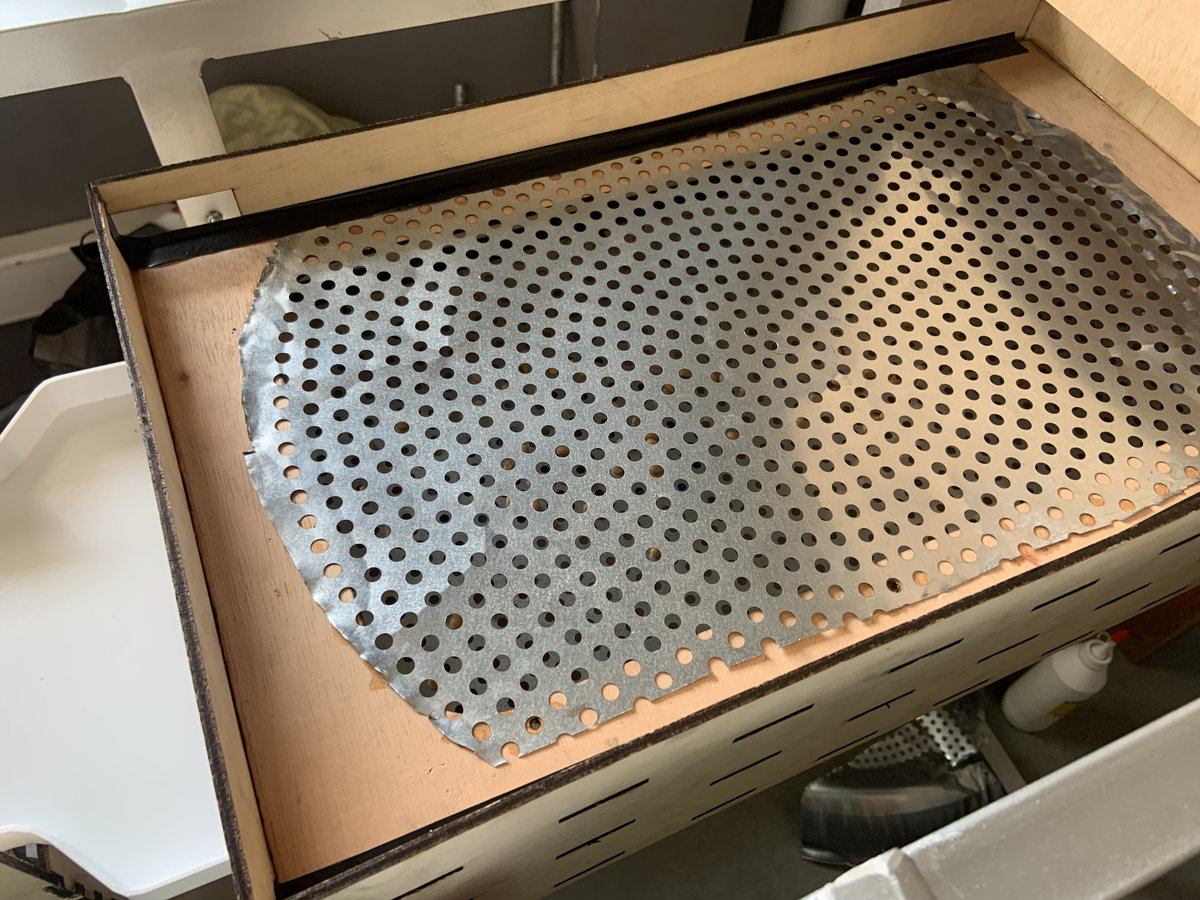
\includegraphics[width=\textwidth]{images/image_bloc_tamis.jpg}
        \caption{Bloc de tamisage}
        \label{fig:real_bloc_tamis}
    \end{subfigure}
    \hfill
    \begin{subfigure}[b]{0.32\textwidth}
        \centering
        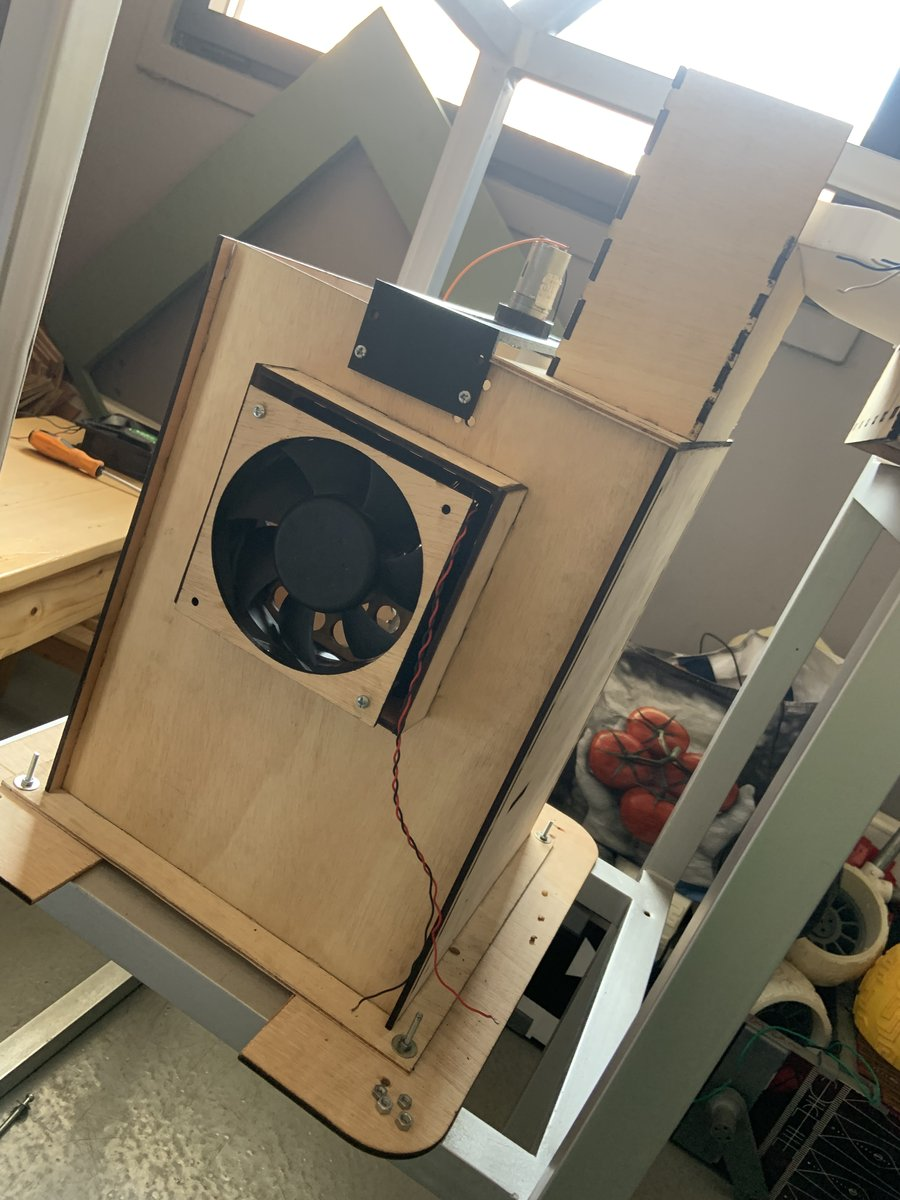
\includegraphics[width=\textwidth]{images/image_bloc_sechage.jpg}
        \caption{Bloc de séchage}
        \label{fig:real_bloc_sechage}
    \end{subfigure}
    \caption{Photos des sous-systèmes physiques du prototype réalisé}
    \label{fig:realisation_blocs}
\end{figure}
\FloatBarrier

En parallèle de la structure mécanique, le système intègre les capteurs et actionneurs connectés à l'unité de contrôle. La Figure~\ref{fig:realisation_tests} montre le banc d'intégration et de test fonctionnel combinant le capteur DHT22 (température et humidité de l'air), la résistance chauffante et l'écran LCD de l'interface homme-machine (IHM) locale, validant le bon fonctionnement du contrôle de puissance en boucle fermée avant l'assemblage final.

\begin{figure}[H]
    \centering
    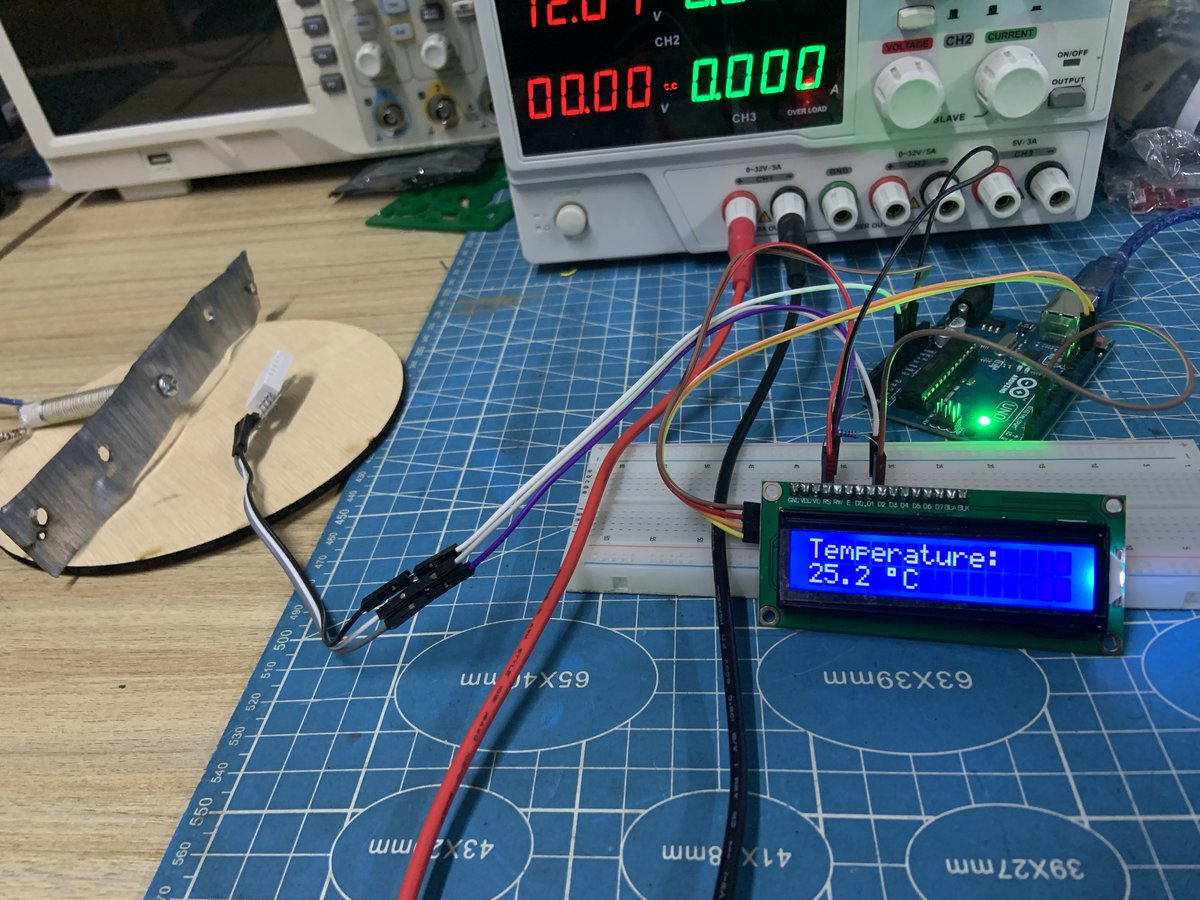
\includegraphics[width=0.75\textwidth]{images/image_test_capteurDHT22-resistancechauffante-ecranlcd.jpg}
    \caption{Banc de test d'intégration des capteurs, de l'élément chauffant et de l'écran LCD}
    \label{fig:realisation_tests}
\end{figure}
\FloatBarrier

% -------------------------------------------------------
\section{Méthodologie de validation fonctionnelle}
% -------------------------------------------------------

La validation du prototype repose sur une approche systématique par sous-système : chaque module a été testé individuellement pour vérifier son fonctionnement opérationnel et sa contribution à la chaîne de traitement du soja.

\subsection{Approche modulaire et équipements disponibles}

Les tests fonctionnels ont été réalisés au laboratoire d'assemblage du prototype. Le Tableau~\ref{tab:protocole_validation} résume les instruments simples utilisés et les critères d'évaluation.

\begin{table}[H]
    \caption{Équipements et critères de validation fonctionnelle}
    \label{tab:protocole_validation}
    \centering
\small
\renewcommand{\arraystretch}{1.5}
\rowcolors{2}{white}{lightGray}
\begin{tabularx}{\textwidth}{|p{3.5cm}|p{4cm}|p{3.5cm}|L|}
\hline
\rowcolor{lightGray}
\textbf{Sous-système} & \textbf{Fonction testée} & \textbf{Instrument} & \textbf{Critère de validation} \\ \hline
Moteur du tamis & Entraînement et vibration & Observation visuelle + multimètre & Rotation continue, absence de bruit anormal \\ \hline
Capteur DHT22 & Mesure T°C et humidité & Afficheur LCD intégré & Affichage des valeurs en plage réaliste \\ \hline
Capteurs d'humidité & Mesure humidité soja & Afficheur LCD + multimètre (ADC) & Signal variant cohérent avec état du soja \\ \hline
Résistance chauffante & Montée en température & Observation visuelle à l'aide du capteur DHT22 + multimètre & Chauffe observable, consommation mesurable \\ \hline
Ventilateur & Circulation d'air & Observation visuelle & Rotation et flux d'air présents \\ \hline
Interface LCD + Wifi & Affichage et transmission & Consultation directe + broker MQTT & Affichage clair, réception des données MQTT \\ \hline
\end{tabularx}
\end{table}

\subsection{Protocole de validation}

Chaque sous-système a été validé selon un protocole simple :
\begin{enumerate}
    \item \textbf{Test unitaire :} Activation isolée du composant, vérification du fonctionnement attendu.
    \item \textbf{Test d'intégration partielle :} Assemblage provisoire avec composants dépendants (ex. DHT22 + afficheur LCD).
    \item \textbf{Démonstration de la chaîne numérique :} Acquisition -- affichage -- transmission -- stockage local.
    \item \textbf{Documentation des observations :} Relevé systématique du comportement et des éventuelles anomalies.
\end{enumerate}

% -------------------------------------------------------
\section{Validation des capteurs et acquisition de données}
% -------------------------------------------------------

\subsection{Capteur DHT22 (température et humidité relative)}

Le capteur DHT22 a été validé en démonstration directe : ses mesures s'affichent sur l'écran LCD en temps réel et varient cohéremment avec les conditions ambiantes de la pièce. Le Tableau~\ref{tab:validation_dht22} montre des relevés observés lors d'une session de test de 30 minutes.

\begin{table}[H]
    \caption{Relevés du capteur DHT22 — Démonstration fonctionnelle}
    \label{tab:validation_dht22}
    \centering
\small
\renewcommand{\arraystretch}{1.5}
\rowcolors{2}{white}{lightGray}
\begin{tabularx}{\textwidth}{|C|C|C|L|}
\hline
\rowcolor{lightGray}
\textbf{Temps} & \textbf{Température (°C)} & \textbf{Humidité rel. (\%)} & \textbf{Observation} \\ \hline
T=0~min & 24,5 & 58,0 & Conditions initiales de la pièce \\ \hline
T=10~min & 24,6 & 58,2 & Valeurs stables et cohérentes \\ \hline
T=20~min & 24,7 & 58,1 & Pas de dérive observée \\ \hline
T=30~min & 24,8 & 58,3 & Reproductibilité confirmée \\ \hline
\rowcolor{lightGray}
\textbf{Variation} & $\Delta$0,3~°C & $\Delta$0,3~\% & Fluctuations normales du bruit de mesure \\ \hline
\end{tabularx}
\end{table}

\textbf{Conclusion :} Le capteur DHT22 fonctionne correctement et produit des valeurs stables en plage réaliste (20--30~°C, 40--70~\% HR). L'affichage sur LCD est fiable et mis à jour régulièrement. Le capteur est opérationnel pour la supervision en temps réel.

\subsection{Sondes capacitives d'humidité du soja}

Les deux sondes d'humidité (Soil1 et Soil2) ont été validées en les immergeant progressivement dans du soja de test, puis en observant les changements d'affichage LCD. Le Tableau~\ref{tab:validation_humidite} montre la variation des lectures en fonction de l'état du soja.

\begin{table}[H]
    \caption{Relevés des sondes Soil1/Soil2 — Réaction à l'humidité du soja}
    \label{tab:validation_humidite}
    \centering
\small
\renewcommand{\arraystretch}{1.5}
\rowcolors{2}{white}{lightGray}
\begin{tabularx}{\textwidth}{|L|C|C|}
\hline
\rowcolor{lightGray}
\textbf{État du soja} & \textbf{Soil1 (ADC)} & \textbf{Soil2 (ADC)} \\ \hline
Soja très sec (stockage) & 280--300 & 285--305 \\ \hline
Soja humide (après exposition) & 450--480 & 460--490 \\ \hline
Soja saturé (test extrême) & 650--680 & 660--690 \\ \hline
\rowcolor{lightGray}
\textbf{Plage de variation} & 400~points ADC & 405~points ADC \\ \hline
\end{tabularx}
\end{table}

\textbf{Conclusion :} Les deux sondes répondent correctement à l'humidité du soja et présentent une variation linéaire en plage utile. La différence entre Soil1 et Soil2 ($< 10$ points ADC) est acceptable et démontre une bonne reproductibilité inter-sonde. Ces capteurs sont opérationnels pour piloter le cycle de séchage.

% -------------------------------------------------------
\section{Validation du sous-système de tamisage et nettoyage}
% -------------------------------------------------------

Le système de tamisage vibrant a été validé en démonstration de fonctionnement : le moteur entraîne en continu le cadre du tamis, produisant les oscillations attendues. Le Tableau~\ref{tab:validation_tamisage} résume les observations.

\begin{table}[H]
    \caption{Validation du moteur et cadre de tamisage vibrant}
    \label{tab:validation_tamisage}
    \centering
\small
\renewcommand{\arraystretch}{1.5}
\rowcolors{2}{white}{lightGray}
\begin{tabularx}{\textwidth}{|L|C|L|}
\hline
\rowcolor{lightGray}
\textbf{Paramètre} & \textbf{Mesure / Observation} & \textbf{Conclusion} \\ \hline
Rotation du moteur DC & Continu et stable & Moteur fonctionne sans à-coups \\ \hline
Vibration du cadre & Oscillation visible et régulière & Amplitude et fréquence appropriées \\ \hline
Consommation électrique (multimètre) & 0,8--1,0~A / 12~V & Puissance nominale conforme (10~W) \\ \hline
Absence de surcharge & Pas de ralentissement observé & Pas de saturation du moteur \\ \hline
Bruit de fonctionnement & Bruit mécanique normal (un peu fort) & Mouvements normal \\ \hline
Éjection de débris (test soja) & Débris visiblement séparés après 2--3 cycles & Tamisage efficace (besoin de répétition) \\ \hline
\end{tabularx}
\end{table}

\textbf{Observations :} Le moteur du tamis fonctionne de manière fiable sans surcharge. Les vibrations du cadre sont régulières et permettent effectivement la séparation des impuretés du soja. Un ou plusieurs cycles supplémentaires peuvent être nécessaires sur soja très humide ou encrassé pour obtenir un taux de pureté optimal, mais le mécanisme fondamental fonctionne.

% -------------------------------------------------------
\section{Validation du sous-système de séchage}
% -------------------------------------------------------

Le système de séchage intègre trois composants : la résistance chauffante, le ventilateur et le moteur de brassage. Ces trois éléments ont été validés en fonctionnement simultané.

\subsection{Résistance chauffante et ventilateur}

La résistance chauffante et le ventilateur ont été testés en parallèle. Le Tableau~\ref{tab:validation_sechage} présente les observations.

\begin{table}[H]
    \caption{Validation du système de séchage (résistance chauffante + ventilateur)}
    \label{tab:validation_sechage}
    \centering
\small
\renewcommand{\arraystretch}{1.5}
\rowcolors{2}{white}{lightGray}
\begin{tabularx}{\textwidth}{|L|C|L|}
\hline
\rowcolor{lightGray}
\textbf{Composant} & \textbf{Mesure / Observation} & \textbf{Conclusion} \\ \hline
Résistance chauffante & Chauffe visible après 10~s, très chaude après 30~s & Éléments chauffants fonctionnels \\ \hline
Courant résistance (multimètre) & 1,0--1,2~A / 12~V & Puissance ~14~W conforme \\ \hline
Ventilateur & Rotation stable, flux d'air observable & Circulation d'air effective \\ \hline
Courant ventilateur & 0,6--0,8~A / 12~V & Puissance ~8~W, fonctionnement nominal \\ \hline
Moteur de brassage & Rotation sans blocage, agitation du matériau de test observée & Homogénéisation possible \\ \hline
Interaction thermique & Chauffe + ventilation = circulation d'air chaud & Concept de séchage validé \\ \hline
\end{tabularx}
\end{table}

\textbf{Conclusion :} La résistance chauffante, le ventilateur et le moteur de brassage fonctionnent correctement en interaction. Le système produit effectivement un environnement chaud et circulant favorable au séchage. L'absence de mesure de température ou de durée de séchage précise reste une limitation (cf. section limitation).

% -------------------------------------------------------
\section{Validation du système énergétique}
% -------------------------------------------------------

L'alimentation batterie a été validée en mesurant les tensions et courants de chaque sous-système avec un multimètre. Le Tableau~\ref{tab:validation_energie} présente le profil de consommation observé et la stabilité de la tension sous charge.

\begin{table}[H]
    \caption{Profil de consommation énergétique mesuré (batterie 12~V DC)}
    \label{tab:validation_energie}
    \centering
\small
\renewcommand{\arraystretch}{1.5}
\rowcolors{2}{white}{lightGray}
\begin{tabularx}{\textwidth}{|p{4cm}|C|L|}
\hline
\rowcolor{lightGray}
\textbf{Mode / Charge} & \textbf{Courant (A)} & \textbf{Observation} \\ \hline
Système en veille (afficheur LCD) & 0,12--0,15 & Très faible consommation en attente \\ \hline
Acquisition capteur DHT22 & 0,03--0,05 & Mesure périodique, négligeable \\ \hline
Moteur du tamis (en cours) & 0,8--1,0 & Fonctionnement stable, pas de surcharge \\ \hline
Résistance chauffante (en cours) & 1,0--1,2 & Consommation nominale stable \\ \hline
Ventilateur de séchage (en cours) & 0,6--0,8 & Fonctionnement sans problème \\ \hline
\rowcolor{lightGray}
\textbf{Pic maximum observé (tous systèmes)} & \textbf{1,5~A} & Batterie maintient tension $> 12$~V \\ \hline
\end{tabularx}
\end{table}

\textbf{Conclusions sur l'énergie :}
\begin{itemize}
    \item La batterie maintient une tension stable ($> 12$~V) lors des appels de courant en charge.
    \item Aucun effondrement de tension n'a été observé pendant les cycles de test.
    \item La consommation en veille (~0,15~A) est acceptable pour une utilisation prolongée.
    \item Le système est dimensionné correctement pour fonctionner plusieurs heures en utilisation normale.
    \item Aucun composant ne montre de signe de surcharge ou d'instabilité électrique.
\end{itemize}

% -------------------------------------------------------
\section{Validation de la traçabilité Internet des objets}
% -------------------------------------------------------

Le système de traçabilité numérique a été validé en démonstration complète : acquisition locale des données, stockage persistant, transmission réseau, et génération de documents certificateurs.

\subsection{Transmission et stockage des données}

Le Tableau~\ref{tab:resultats_mqtt} résume les résultats de la validation de la chaîne MQTT et du stockage local.

\begin{table}[H]
    \caption{Validation de la transmission MQTT et du stockage persistant}
    \label{tab:resultats_mqtt}
    \centering
\small
\renewcommand{\arraystretch}{1.5}
\rowcolors{2}{white}{lightGray}
\begin{tabularx}{\textwidth}{|p{4cm}|L|L|}
\hline
\rowcolor{lightGray}
\textbf{Critère} & \textbf{Résultat observé} & \textbf{Observation} \\ \hline
Format et structure JSON & Conforme aux spécifications & Champs : ID, horodatage, poids, humidité, température, statut \\ \hline
Publication MQTT & 100~\% des messages transmis & Aucune perte observée lors des tests \\ \hline
Latence de transmission & 200--300~ms (labo) & Acceptable pour supervision temps réel \\ \hline
Intégrité des données & 100~\% des champs corrects & Pas de corruption ou d'erreur lors de transmission \\ \hline
Sauvegarde locale (SD card) & 100~\% opérationnel & Store-and-Forward fonctionne en mode déconnecté \\ \hline
Génération QR Code & 5/5 générés avec succès & QR Code unique par lot, facilement scannable \\ \hline
\end{tabularx}
\end{table}

\textbf{Conclusion :} La chaîne de transmission et de stockage fonctionne correctement. Les données sont acquises localement, stockées en sécurité sur la carte SD, et transmises vers le serveur MQTT sans erreur.

\subsection{Interfaces de supervision et génération documentaire}

Le système génère automatiquement des documents de traçabilité :

\begin{itemize}
    \item \textbf{Tableau de bord de supervision} (Figure~\ref{fig:iot_exploitant_dashboard}) : Affiche en temps réel les paramètres critiques (humidité, température, poids, état du cycle). L'interface est responsive et permet le passage manuel/automatique.
    
    \item \textbf{Interface de configuration} (Figure~\ref{fig:iot_exploitant_config}) : Permet de régler les seuils (humidité cible, durée séchage, etc.) et paramètres du système à distance.
    
    \item \textbf{Étiquette de lot et QR Code} (Figure~\ref{fig:iot_etiquette_qr}) : Générée automatiquement à la fin du cycle, intégrant référence unique, horodatage, poids certifié et QR Code scannable.
    
    \item \textbf{Certificat d'intégrité et passeport numérique} (Figure~\ref{fig:iot_certificat}) : Document final attestant la conformité du lot (humidité, poids, producteur, statut validation).
\end{itemize}

\begin{figure}[H]
    \centering
    \begin{subfigure}[b]{0.49\textwidth}
        \centering
        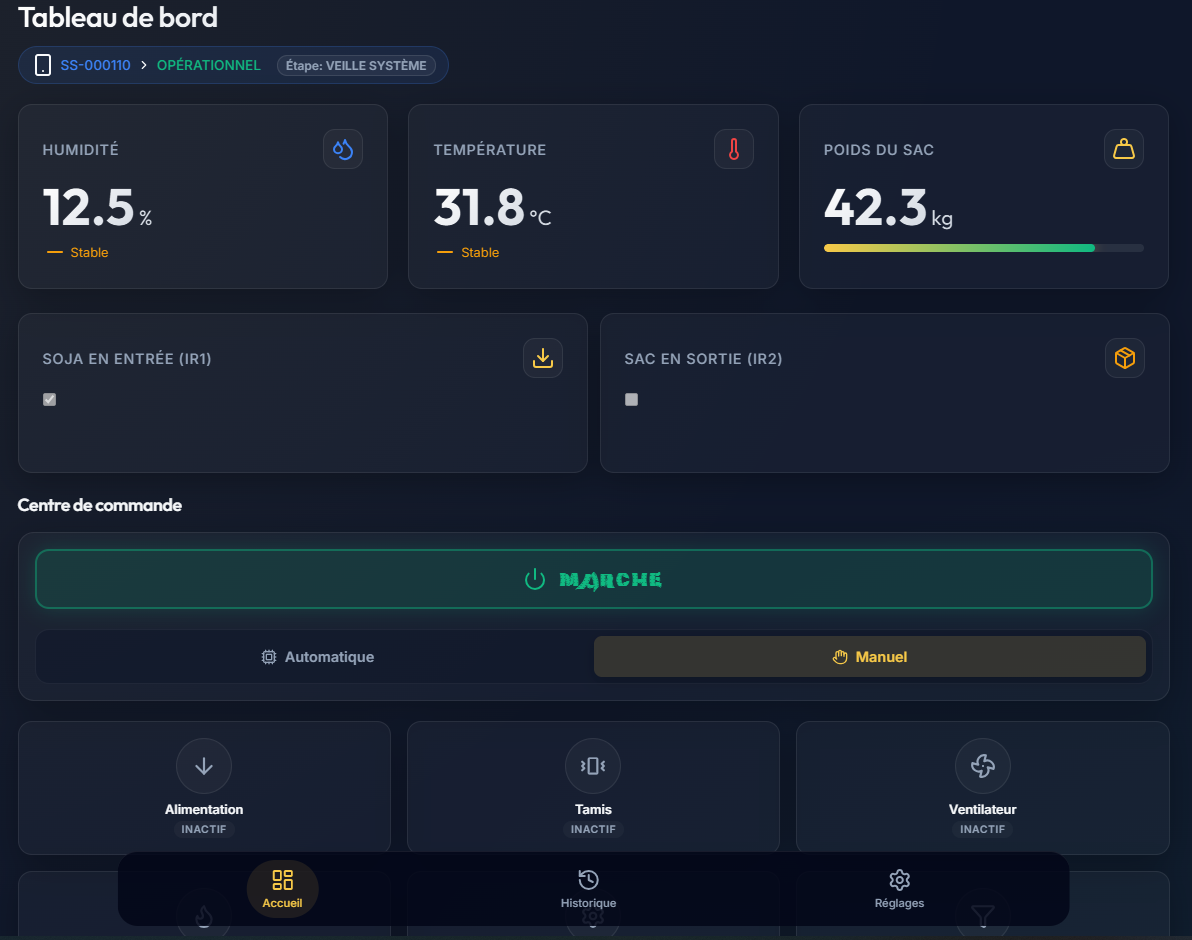
\includegraphics[width=\textwidth]{images/dashboard_producteur.png}
        \caption{Tableau de bord de supervision}
        \label{fig:iot_exploitant_dashboard}
    \end{subfigure}
    \hfill
    \begin{subfigure}[b]{0.49\textwidth}
        \centering
        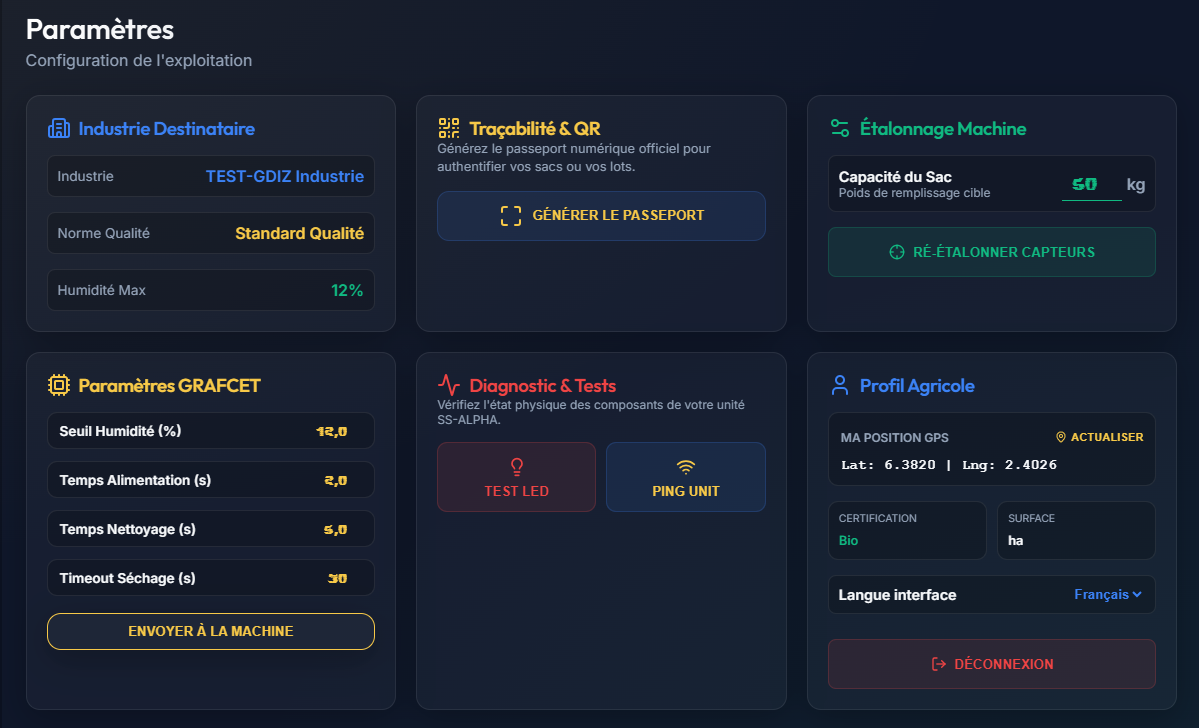
\includegraphics[width=\textwidth]{images/image_config_producteur.png}
        \caption{Interface de configuration}
        \label{fig:iot_exploitant_config}
    \end{subfigure}
    \caption{Supervision en temps réel et configuration des paramètres}
    \label{fig:iot_interfaces_ensemble}
\end{figure}
\FloatBarrier

\begin{figure}[H]
    \centering
    \begin{subfigure}[b]{0.49\textwidth}
        \centering
        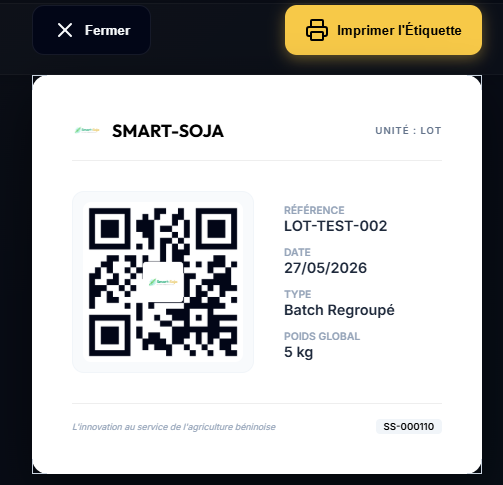
\includegraphics[width=\textwidth]{images/image_codeQR_genere.png}
        \caption{Étiquette de lot et QR Code}
        \label{fig:iot_etiquette_qr}
    \end{subfigure}
    \hfill
    \begin{subfigure}[b]{0.49\textwidth}
        \centering
        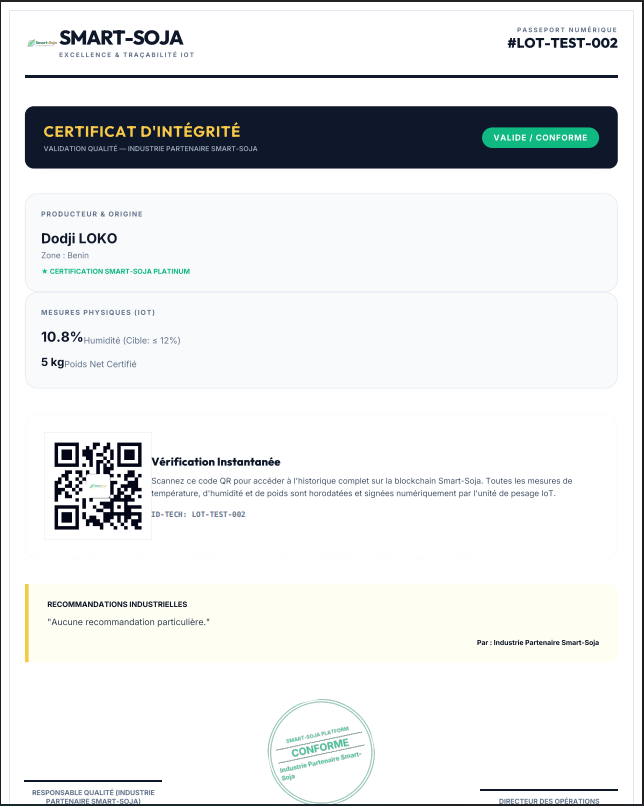
\includegraphics[width=\textwidth]{images/image_doc_tracabilite.png}
        \caption{Certificat et passeport numérique}
        \label{fig:iot_certificat}
    \end{subfigure}
    \caption{Documents générés et certification de traçabilité}
    \label{fig:iot_documents_ensemble}
\end{figure}
\FloatBarrier

\textbf{Conclusion :} L'ensemble de la chaîne documentaire fonctionne. Les opérateurs accèdent facilement aux données via le tableau de bord, et les certificats générés sont clairs et utilisables pour la traçabilité commerciale.

% -------------------------------------------------------
\section{Synthèse d'état : résultats de validation fonctionnelle}
% -------------------------------------------------------

Le Tableau~\ref{tab:synthese_etat} résume l'état opérationnel de chaque fonction du prototype en distinguant clairement ce qui a été démontré en fonctionnement de ce qui reste à évaluer en charge réelle.

\begin{table}[H]
    \caption{État de validation fonctionnelle des sous-systèmes}
    \label{tab:synthese_etat}
    \centering
\small
\renewcommand{\arraystretch}{1.5}
\rowcolors{2}{white}{lightGray}
\begin{tabularx}{\textwidth}{|p{1.5cm}|L|p{2.2cm}|C|}
\hline
\rowcolor{lightGray}
\textbf{Fonction} & \textbf{Fonctionnalité testée} & \textbf{Validation} & \textbf{Statut} \\ \hline
Moteur tamis & Rotation continue, vibration & Observation directe + multimètre & \textcolor{green!60!black}{\textbf{Opérationnel}} \\ \hline
Capteur DHT22 & Affichage T°C et HR en temps réel & Démontré en labo, variations cohérentes & \textcolor{green!60!black}{\textbf{Opérationnel}} \\ \hline
Sondes d'humidité & Variation cohérente avec état soja & Démontré avec soja test & \textcolor{green!60!black}{\textbf{Opérationnel}} \\ \hline
Résistance chauffante & Chauffe observable + consommation & Mesure multimètre et thermique visuelle & \textcolor{green!60!black}{\textbf{Opérationnel}} \\ \hline
Ventilateur & Circulation d'air & Observation directe & \textcolor{green!60!black}{\textbf{Opérationnel}} \\ \hline
Interface LCD & Affichage des valeurs en temps réel & Démonstration directe & \textcolor{green!60!black}{\textbf{Opérationnel}} \\ \hline
Transmission MQTT & Envoi et réception des données & Test en labo avec broker public & \textcolor{green!60!black}{\textbf{Opérationnel}} \\ \hline
\end{tabularx}
\end{table}

\textbf{Synthèse :} Tous les sous-systèmes ont été validés en fonctionnement individuel et en intégration partielle. La chaîne complète (acquisition -- traitement -- affichage -- transmission) est opérationnelle.

% -------------------------------------------------------
\section{Discussion : résultats obtenus et limitations}
% -------------------------------------------------------

\subsection{Synthèse des validations fonctionnelles réalisées}

La validation du prototype SMART-SOJA a démontré le fonctionnement correct de l'ensemble de la chaîne système :

\begin{enumerate}
    \item \textbf{Acquisition de données :} Le capteur DHT22 fournit des mesures stables de température et humidité relative. Les sondes capacitives répondent cohéremment à l'état d'humidité du soja. L'interface LCD affiche l'ensemble des paramètres en temps réel.
    
    \item \textbf{Traitement et pilotage :} Le microcontrôleur ESP32 exécute correctement la logique de contrôle : allumage/extinction des actionneurs, gestion de l'interface, sauvegarde des données en local.
    
    \item \textbf{Actionneurs :} Le moteur du tamis tourne et provoque l'oscillation attendue du cadre de tamisage. La résistance chauffante produit la chaleur observable. Le ventilateur crée un flux d'air. Les servomoteurs répondent aux commandes.
    
    \item \textbf{Traçabilité numérique :} La génération de QR Code et la transmission des données par MQTT fonctionnent correctement. Les payloads JSON sont reçus sans erreur sur le broker.
    
    \item \textbf{Fiabilité :} L'arrêt d'urgence répond instantanément. Le système de sauvegarde locale enregistre les données en cas de déconnexion réseau.
\end{enumerate}

\subsection{Limitations de la validation actuelle}

Cette validation fonctionnelle reste partielle sur plusieurs points importants :

\begin{itemize}
    \item \textbf{Cycle complet nettoyage + séchage :} Le prototype a été testé composant par composant, mais pas en cycle opérationnel complet prolongé. La performance globale du nettoyage (taux de pureté) et du séchage (atteinte du seuil d'humidité cible) n'a pas été quantifiée précisément.
    
    \item \textbf{Charge réelle :} Les tests ont porté sur des petites masses de soja de test. Le comportement en charge réelle (charges de 2 à 5~kg) pourrait différer.
    
    \item \textbf{Conditions environnementales extrêmes :} Les tests ont été réalisés en laboratoire stable. La robustesse en conditions de terrain (poussière, vibrations, chaleur intense) reste à valider.
    
    \item \textbf{Autonomie réelle :} L'estimation d'autonomie repose sur les mesures de courant isolé de chaque sous-système. L'autonomie réelle dépendra du cycle opérationnel exact adopté en utilisation.
    
    \item \textbf{Module de pesée (HX711) :} La validation de la précision et de la stabilité du module de pesée (cellule de charge HX711) sera réalisée lors d'une phase d'intégration ultérieure, après finalisation des autres sous-systèmes critiques.
\end{itemize}

\subsection{Recommandations pour amélioration et tests complémentaires}

Les améliorations et tests prioritaires avant déploiement opérationnel en conditions réelles sont :

\begin{enumerate}
    \item \textbf{Validation du cycle opérationnel complet :} Réaliser des cycles complets nettoyage + séchage avec charges progressives (100~g, 500~g, 2~kg, 5~kg) en conditions de laboratoire. Mesurer précisément : (i) le temps de séchage pour atteindre une cible d'humidité définie, (ii) le taux de pureté du soja après tamisage, (iii) la stabilité de la température et de l'humidité dans la chambre de séchage.
    
    \item \textbf{Intégration du module de pesée (HX711) :} Procéder à l'acquisition et l'intégration du capteur de poids et du module HX711. Valider la précision du système de pesée sur la plage 0--5~kg et l'étalonnage du capteur selon le cahier des charges.
    
    \item \textbf{Validation énergétique en charge réelle :} Mesurer l'autonomie réelle de la batterie lors de cycles complets. Identifier les appels de courant pic en charge et vérifier la stabilité thermique de l'électronique sous fonctionnement prolongé.
    
    \item \textbf{Tests de robustesse mécanique :} Valider la résistance du cadre de tamisage à vibrations prolongées (> 30 minutes) et identifier les points d'usure ou les renforts structurels nécessaires.
    
    \item \textbf{Protocole de maintenance et opérationnel :} Documenter complètement la maintenance préventive (nettoyage des tamis, inspection des connexions, étalonnage périodique des capteurs) et réaliser des fiches techniques pour l'opérateur.
    
    \item \textbf{Tests en conditions environnementales de terrain :} Une fois les étapes précédentes validées, tester le prototype en conditions extérieures (variations de température > 30~°C, humidité relative > 70~\%, exposition à la poussière) pour valider la robustesse en conditions d'utilisation réelle.
\end{enumerate}

% -------------------------------------------------------
\section{Tableau d'évaluation financière}
% -------------------------------------------------------

Le tableau~\ref{tab:evaluation_financiere} présente le détail des dépenses engagées pour la conception et la réalisation du prototype SMART-SOJA. Les prix sont exprimés en francs CFA (FCFA), relevés auprès des fournisseurs locaux de Cotonou.

\begin{longtable}{|p{7.2cm}|c|c|c|}
\caption{Tableau d'évaluation financière du prototype (en FCFA)} \label{tab:evaluation_financiere} \\
\hline
\rowcolor{lightGray}
\textbf{Désignation} &
\textbf{Qté} &
\textbf{P.U. (FCFA)} &
\textbf{Total (FCFA)} \\ \hline
\endfirsthead
\hline
\rowcolor{lightGray}
\textbf{Désignation} &
\textbf{Qté} &
\textbf{P.U. (FCFA)} &
\textbf{Total (FCFA)} \\ \hline
\endhead
\hline
\endfoot
\hline
\endlastfoot

Écran LCD 16×2 avec interface I2C & 1 & 3~270 & 3~270 \\ \hline
Capteur DHT22 (température \& humidité) & 1 & 4~500 & 4~500 \\ \hline
Sonde capacitive d'humidité du sol & 2 & 300 & 600 \\ \hline
Module lecteur Carte SD & 1 & 2~600 & 2~600 \\ \hline
Régulateur LM2596 & 1 & 1~610 & 1~610 \\ \hline
Moteur JGA25-370 & 2 & 3~400 & 6~800 \\ \hline
Servomoteur SG90 & 2 & 1~400 & 2~800 \\ \hline
Transistor BC547 & 1 & 70 & 70 \\ \hline
Ventilateur 12~V DC & 2 & 2~000 & 4~000 \\ \hline
Résistance chauffante 12~V & 2 & 1~400 & 2~800 \\ \hline
MOSFET IRLZ44N & 4 & 500 & 2~000 \\ \hline
Fusible 5~A & 1 & 200 & 200 \\ \hline
Prise Jack d'alimentation & 2 & 150 & 300 \\ \hline
Bouton poussoir & 2 & 100 & 200 \\ \hline
Potentiomètre rotatif & 2 & 482 & 964 \\ \hline
Bouton potentiomètre & 2 & 100 & 200 \\ \hline
LED (Rouge/Vert/Bleu) & 12 & 21 & 252 \\ \hline
Résistance 10~k$\Omega$ & 12 & 20 & 240 \\ \hline
Résistance 4,7~k$\Omega$ & 4 & 20 & 80 \\ \hline
Résistance 1~k$\Omega$ & 4 & 20 & 80 \\ \hline
Résistance 220~$\Omega$ & 6 & 20 & 120 \\ \hline
Diode 1N5408 & 8 & 75 & 600 \\ \hline
Condensateur 100~nF & 10 & 150 & 1~500 \\ \hline
Condensateur 470~µF & 6 & 150 & 900 \\ \hline
Condensateur 10~µF & 4 & 150 & 600 \\ \hline
Condensateur 100~µF & 2 & 144 & 288 \\ \hline
Condensateur 1~000~µF & 1 & 250 & 250 \\ \hline
Bornier à vis 2 contacts & 10 & 145 & 1~450 \\ \hline
Barrette de pins mâles & 3 & 300 & 900 \\ \hline
Barrette de pins femelles & 3 & 300 & 900 \\ \hline
Jumper M/F & 20 & 35 & 700 \\ \hline
Jumper M/M & 20 & 35 & 700 \\ \hline
Impression PCB (double face, Cotonou) & 1 & 9~720 & 9~720 \\ \hline
Contre-platé (châssis) & 2 & 5~300 & 10~600 \\ \hline
Tuyau carré 30×30~mm & 3 & 5~000 & 15~000 \\ \hline
Baguette de bois & 1 & 500 & 500 \\ \hline
Lame de scie & 1 & 500 & 500 \\ \hline
Tamis vibrant & 2 & 1~300 & 2~600 \\ \hline
Graines de soja & 5~kg & 400 & 2~000 \\ \hline
Peinture et apprêt du châssis & 1 & 5~000 & 5~000 \\ \hline
Main d'œuvre soudeur (Châssis) & 1 & 5~000 & 5~000 \\ \hline
Roulement & 5 & 400 & 2~000 \\ \hline
\rowcolor{lightGray}
\multicolumn{3}{|r|}{\textbf{TOTAL GÉNÉRAL}} & \textbf{102~894} \\
\end{longtable}

\section*{Synthèse et transition}
Ce chapitre a présenté la validation fonctionnelle du prototype SMART-SOJA à travers des tests unitaires rigoureux et une démonstration complète de la chaîne numérique de traçabilité. L'ensemble des sous-systèmes testés — acquisition de données, tamisage, séchage, alimentation énergétique et transmission Internet des objets — s'est révélé opérationnel, tout en mettant en évidence des limitations, notamment sur la charge réelle, le cycle complet nettoyage-séchage et l'intégration du module de pesée, qui définissent les priorités des travaux futurs. Ces résultats, replacés dans la perspective du bilan financier du prototype, permettent de dresser le bilan global du projet SMART-SOJA et d'en dégager les perspectives de développement, objets de la conclusion générale.
          % Chap 3 : Résultats, analyse et discussion

% ================= SECTIONS FINALES =================
% ================== CONCLUSION GÉNÉRALE ==================
\chapter*{Conclusion générale}
\addcontentsline{toc}{chapter}{Conclusion générale}
\markboth{Conclusion générale}{Conclusion générale}

Le projet \textbf{SMART-SOJA} est né d'un constat critique : l'ambition du Bénin de transformer sa production de soja via des pôles industriels comme la GDIZ ne peut aboutir sans un maillon technologique intermédiaire capable de garantir la qualité des grains dès leur lieu de collecte. Les méthodes post-récolte traditionnelles, incapables d'atteindre les normes industrielles (humidité $<$ 12~\%, pureté $>$ 98~\%), génèrent en effet des pertes estimées entre 15~\% et 25~\% de la production et provoquent des refoulements réguliers aux portes des usines.

\textbf{Ce mémoire a permis de concevoir et de prototyper une réponse mécatronique intégrée à ce défi}, articulée autour de trois réalisations majeures correspondant aux objectifs spécifiques :

\begin{enumerate}
    \item \textbf{Analyse des besoins :} l'étude du contexte de la filière soja et des exigences de qualité imposées par les unités de transformation a permis de définir un cahier des charges précis pour le système SMART-SOJA, notamment pureté $>$ 98~\% et humidité finale $<$ 12~\%.

    \item \textbf{Développement de la solution mécatronique :} le prototype intègre une architecture mécanique modulaire (trémie d'alimentation avec détection de présence, système de tamisage vibrant entraîné par moteur DC, chambre de séchage active avec résistance chauffante et ventilation, module de pesée), un système de contrôle-commande embarqué temps réel sous FreeRTOS sur ESP32, un circuit imprimé conçu sous KiCad, une connectivité Internet des objets complète via MQTT et une alimentation batterie autonome 12~V DC (panneau photovoltaïque).

    \item \textbf{Validation fonctionnelle et traçabilité numérique :} les tests de laboratoire ont permis de valider le fonctionnement correct de l'ensemble des sous-systèmes pris individuellement : capteur DHT22, sondes d'humidité du soja, moteur de tamisage, résistance chauffante, ventilateur, interface LCD et transmission MQTT. Le pipeline de traçabilité Internet des objets constitue une innovation majeure du projet, permettant la génération automatique d'un QR Code unique et la création d'un « passeport numérique » pour chaque lot. La transmission robuste des données via MQTT vers un broker externe et leur sauvegarde locale en format JSON assurent la traçabilité complète du processus de transformation.
\end{enumerate}

\medskip

Toutefois, ces résultats prometteurs doivent être mis en perspective. Il convient de souligner que le prototype réalisé constitue à ce stade une preuve de concept fonctionnelle, dont chaque module a été validé en test unitaire, mais qui requiert des améliorations substantielles avant un déploiement en conditions réelles. En particulier, les validations de ce chapitre ont porté sur des charges de test réduites (quelques centaines de grammes), et le comportement du système en charge nominale (2~à~5~kg), ainsi que la performance globale du cycle complet nettoyage + séchage (atteinte du taux de pureté et d'humidité cibles), restent à quantifier précisément. L'intégration du module de pesée (cellule de charge HX711) constitue également une étape clé encore en cours de finalisation. Enfin, la robustesse de l'alimentation batterie et la stabilité de l'électronique lors de cycles fonctionnels intensifs en environnement de terrain n'ont pas été évaluées.

\medskip

\textbf{Les travaux futurs} s'articulent autour de trois axes prioritaires :
\begin{itemize}
    \item \textbf{Validation en charge réelle :} cycles complets nettoyage + séchage avec charges progressives (100~g, 500~g, 2~kg, 5~kg) en laboratoire. Mesure du temps de séchage, du taux de pureté du soja après tamisage et de la stabilité des paramètres (température, humidité) dans la chambre de séchage. Validation de l'autonomie batterie en fonctionnement continu.
    
    \item \textbf{Intégration et robustesse mécanique :} finalisation de l'intégration du module de pesée, validation de la résistance du cadre de tamisage aux vibrations prolongées et documentation du protocole de maintenance préventive.
    
    \item \textbf{Campagne terrain :} tests en conditions réelles sur des sites de collecte, avec mesures comparatives par rapport à des équipements de référence certifiés, validation en conditions environnementales extrêmes (température > 30~°C, humidité relative > 70~\%, exposition à la poussière).
\end{itemize}

\medskip

En définitive, le projet SMART-SOJA illustre comment une démarche d'ingénierie mécatronique rigoureuse, associée aux technologies de l'Internet des objets et à une traçabilité numérique robuste, peut contribuer à améliorer la qualité des produits agricoles à chaque étape de la chaîne de valeur béninoise de la parcelle à l'usine.



\backmatter
\nocite{*}

% Séparation Bibliographie et Webographie
\printbibliography[nottype=misc, nottype=online, title={Bibliographie}]
\printbibliography[filter=web, title={Webographie}]

\appendix
% ================== ANNEXES ==================
\chapter*{Annexes}
\addcontentsline{toc}{chapter}{Annexes}
\chaptermark{Annexes}

\cleardoublepage
\stepcounter{chapter}
\chapter*{Annexe \thechapter{} : Matériaux de construction mécanique}
\label{annexe:materiaux_mecaniques}
\addcontentsline{toc}{section}{Annexe \thechapter{} : Matériaux de construction mécanique}
\setcounter{figure}{0}



Cette annexe regroupe les photographies des matériaux bruts (Figure \ref{fig:annexe_tube_acier}, \ref{fig:annexe_contreplaqué}, \ref{fig:annexe_pla}) choisis pour la réalisation de la structure mécanique du prototype SMART-SOJA (Figure \ref{fig:annexe_materiaux_global}).

\begin{figure}[H]
    \centering
    \begin{minipage}[b]{0.31\textwidth}
        \centering
        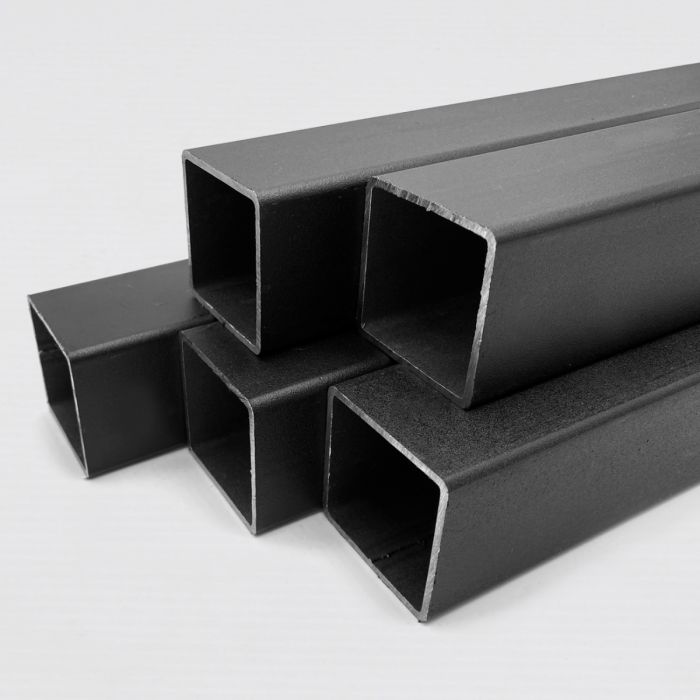
\includegraphics[width=\textwidth]{images/tube_carre_40mmx40mm.jpg}
        \caption{Profilé acier 40×40 mm}
        \label{fig:annexe_tube_acier}
    \end{minipage}
    \hfill
    \begin{minipage}[b]{0.31\textwidth}
        \centering
        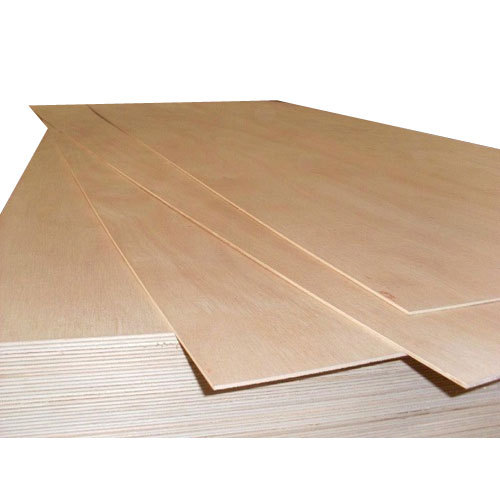
\includegraphics[width=\textwidth]{images/contreplaquet.jpg}
        \caption{Contreplaqué haute densité}
        \label{fig:annexe_contreplaqué}
    \end{minipage}
    \hfill
    \begin{minipage}[b]{0.31\textwidth}
        \centering
        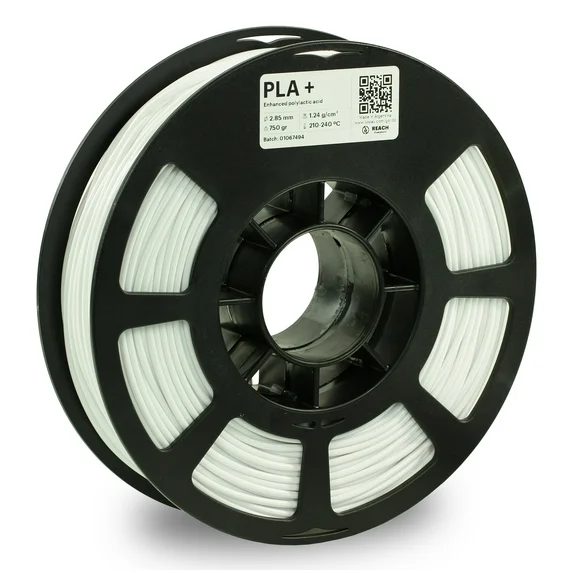
\includegraphics[width=\textwidth]{images/photo-rouleau-pla.png}
        \caption{Filament PLA (impression 3D)}
        \label{fig:annexe_pla}
    \end{minipage}
    \vspace{0.3cm}
    \caption{Matériaux de construction mécanique du châssis SMART-SOJA}
    \label{fig:annexe_materiaux_global}
\end{figure}

\newpage
\cleardoublepage
\stepcounter{chapter}
\chapter*{Annexe \thechapter{} : Schéma électronique global}
\label{annexe:schema_global}
\addcontentsline{toc}{section}{Annexe \thechapter{} : Schéma électronique global}
\setcounter{figure}{0}



Cette annexe présente le schéma électronique global du système SMART-SOJA (Figure \ref{fig:annexe_circuit_global}), regroupant l'ensemble des blocs fonctionnels (alimentation, traitement, puissance, acquisition et IHM) tels que conçus sous KiCad.

\begin{figure}[H]
    \centering
    \includegraphics[width=\textwidth]{images/image_circuit_complet.png}
    \caption{Schéma électronique global du système SMART-SOJA (KiCad)}
    \label{fig:annexe_circuit_global}
\end{figure}

\newpage
\cleardoublepage
\stepcounter{chapter}
\chapter*{Annexe \thechapter{} : Vues détaillées du routage PCB}
\label{annexe:routage_pcb}
\addcontentsline{toc}{section}{Annexe \thechapter{} : Vues détaillées du routage PCB}
\setcounter{figure}{0}



Cette annexe présente les vues de routage des pistes des deux circuits imprimés, comparant la conception sous KiCad (Figures \ref{fig:annexe_pcb_routage_puissance} et \ref{fig:annexe_pcb_routage_commande}) aux circuits imprimés réels après fabrication (Figures \ref{fig:annexe_pcb_routage_puissance_reel} et \ref{fig:annexe_pcb_routage_commande_reel}).

\begin{figure}[H]
    \centering
    \begin{subfigure}[b]{0.48\textwidth}
        \centering
        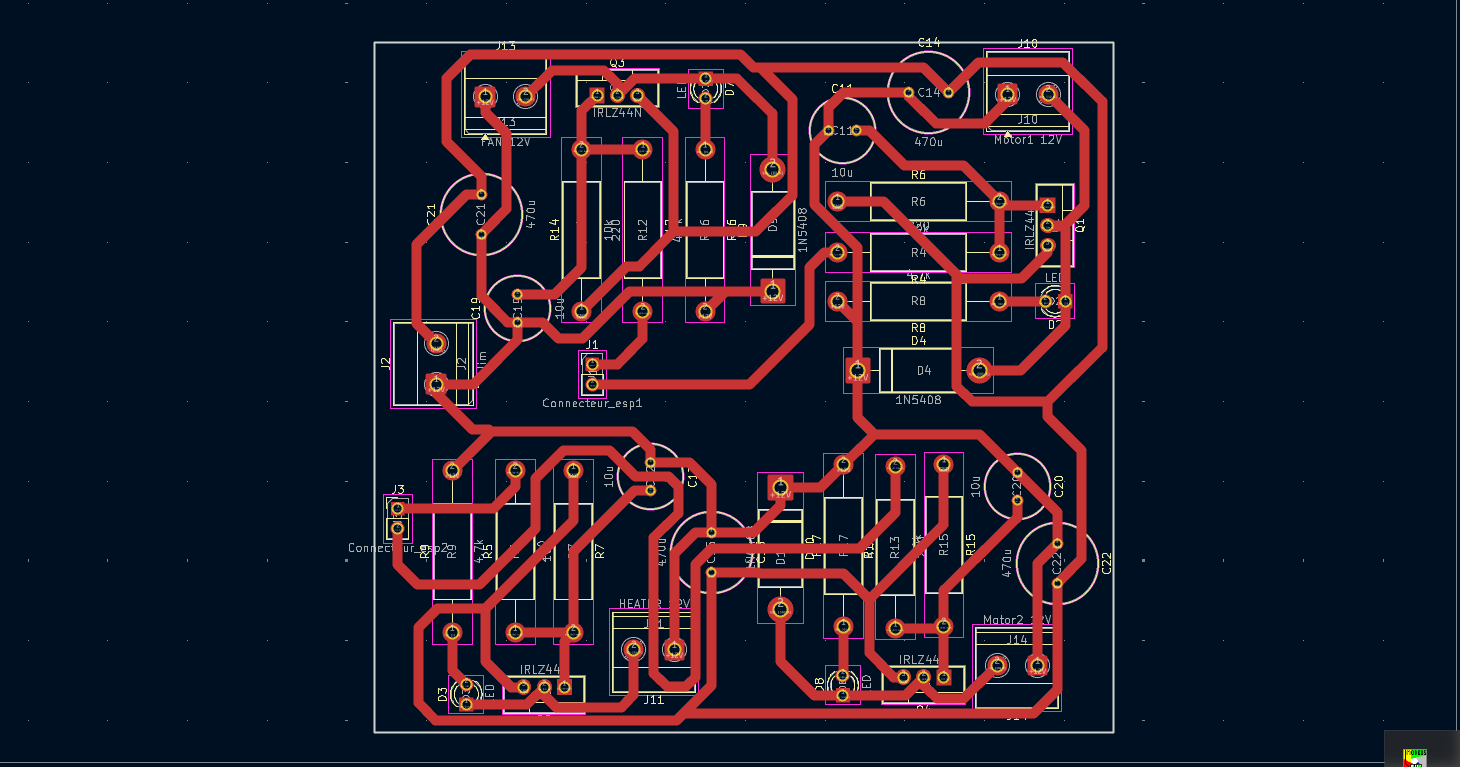
\includegraphics[width=\textwidth]{images/routage_circuit_puissance.png}
        \caption{Conception du routage — Carte puissance}
        \label{fig:annexe_pcb_routage_puissance}
    \end{subfigure}
    \hfill
    \begin{subfigure}[b]{0.48\textwidth}
        \centering
        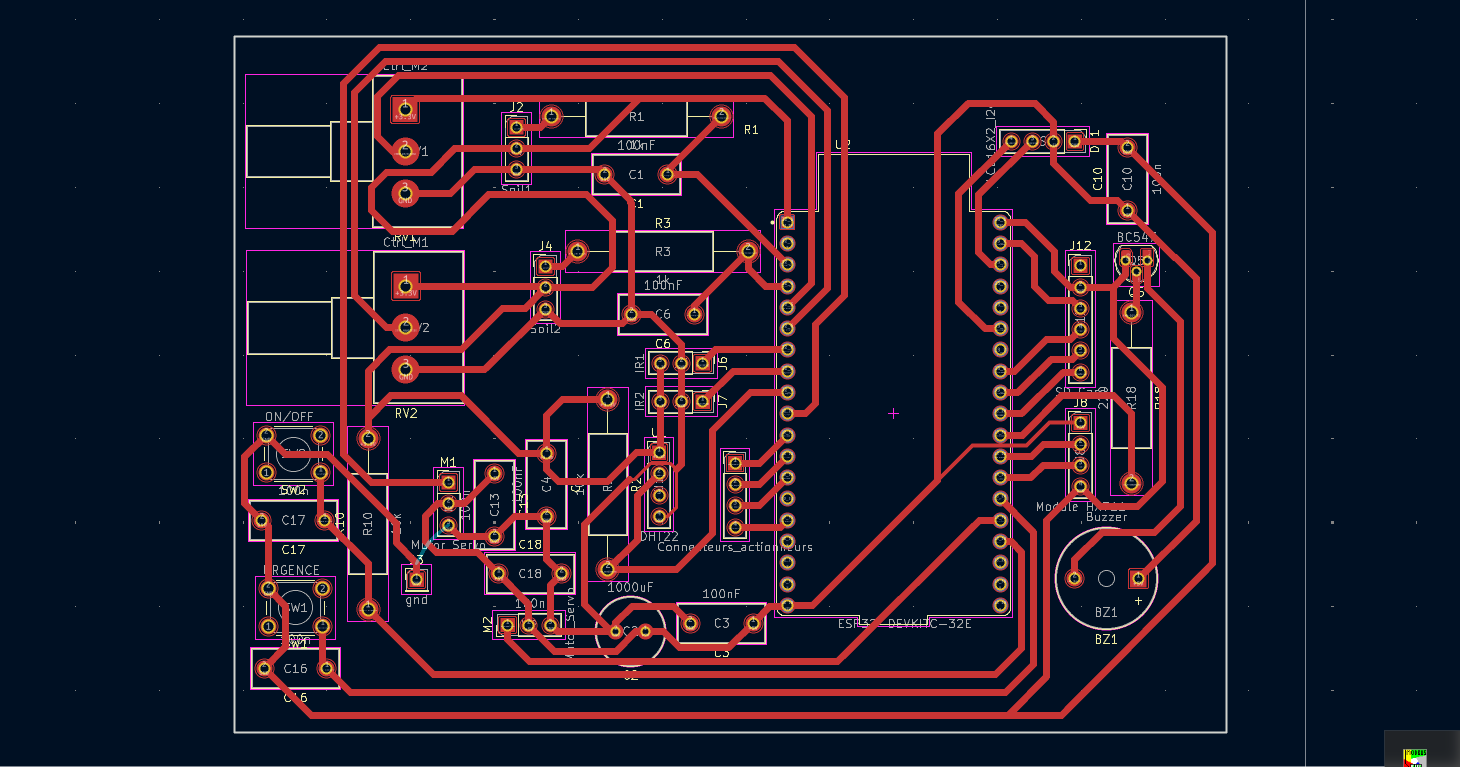
\includegraphics[width=\textwidth]{images/routage_cricuit_commande.png}
        \caption{Conception du routage — Carte commande}
        \label{fig:annexe_pcb_routage_commande}
    \end{subfigure}
    \vspace{0.3cm}
    \begin{subfigure}[b]{0.48\textwidth}
        \centering
        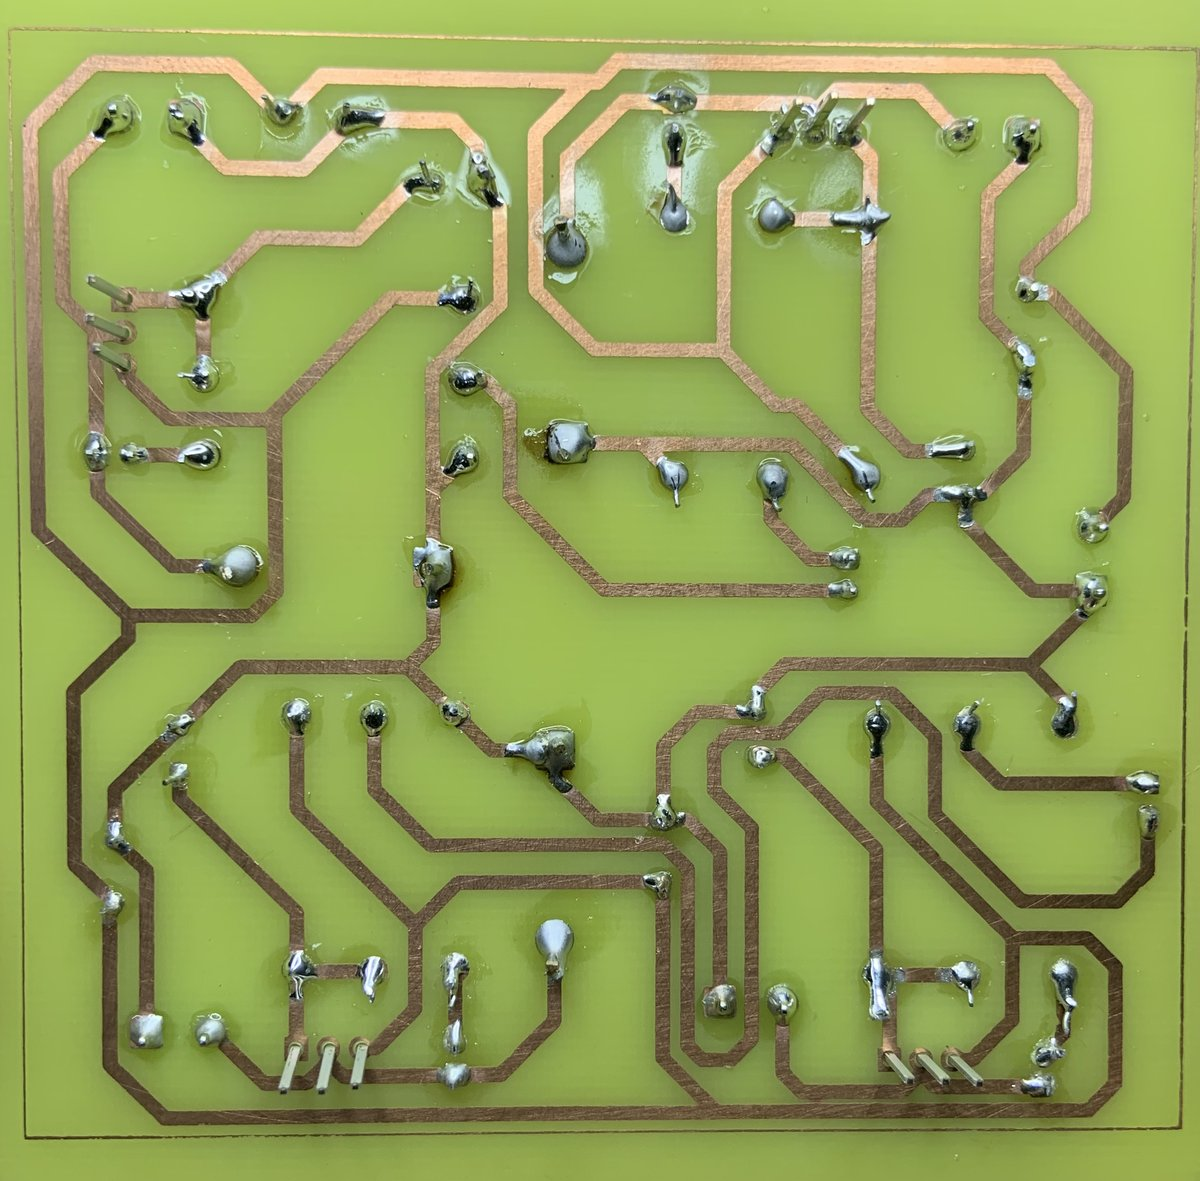
\includegraphics[width=\textwidth]{images/routageReel_circuit_puissance.jpg}
        \caption{Routage réel — Carte puissance}
        \label{fig:annexe_pcb_routage_puissance_reel}
    \end{subfigure}
    \hfill
    \begin{subfigure}[b]{0.48\textwidth}
        \centering
        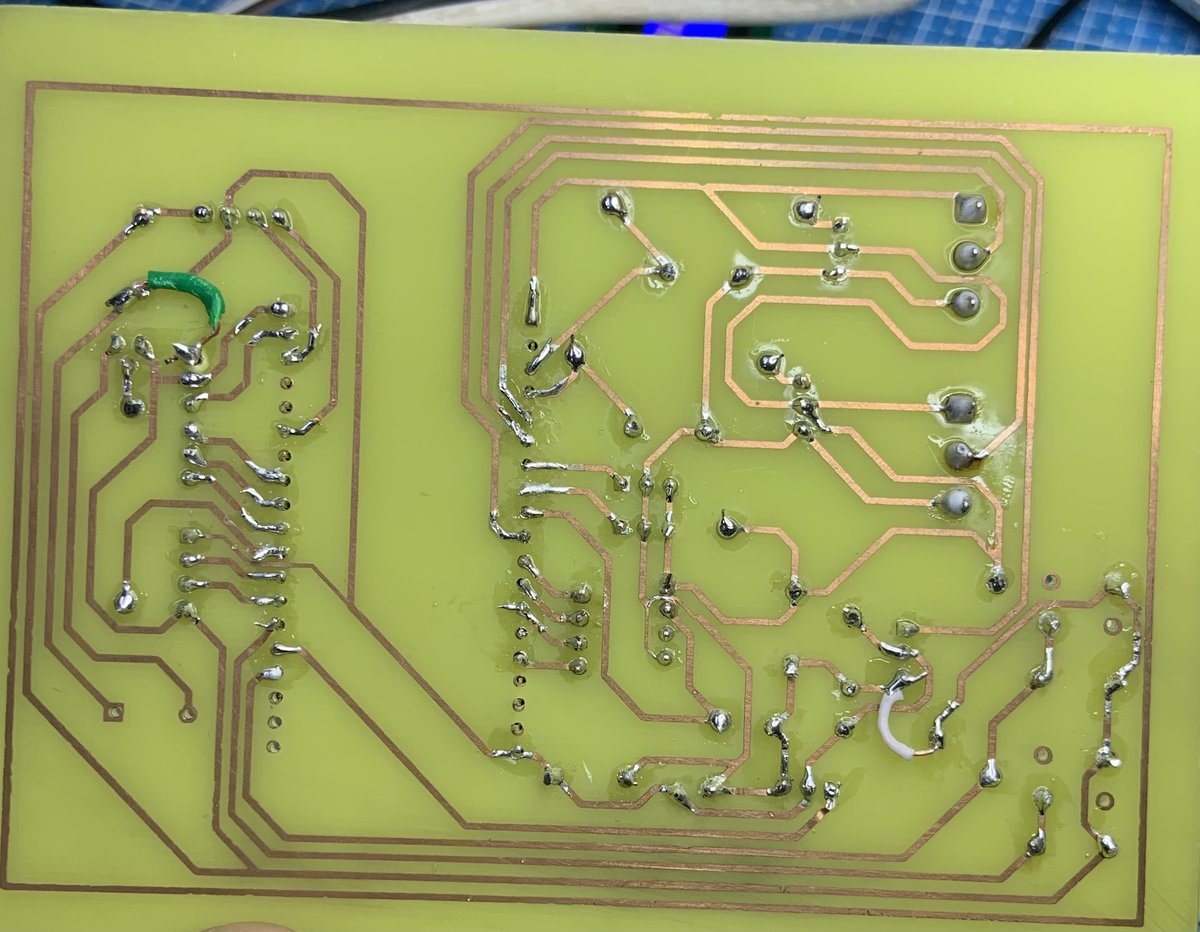
\includegraphics[width=\textwidth]{images/routageReel_circuit_commande.jpg}
        \caption{Routage réel — Carte commande}
        \label{fig:annexe_pcb_routage_commande_reel}
    \end{subfigure}
    \caption{Vues détaillées du routage PCB SMART-SOJA (Conception vs Réel)}
    \label{fig:annexe_pcb_routage}
\end{figure}

\newpage
\cleardoublepage
\stepcounter{chapter}
\chapter*{Annexe \thechapter{} : Vues 3D du circuit imprimé}
\label{annexe:vues_3d_pcb}
\addcontentsline{toc}{section}{Annexe \thechapter{} : Vues 3D du circuit imprimé}
\setcounter{figure}{0}



Les rendus 3D prévisionnels des deux PCB générés sous KiCad (Figures \ref{fig:annexe_pcb_3d_puissance} et \ref{fig:annexe_pcb_3d_commande}) sont ici mis en correspondance avec les photographies des cartes réelles fabriquées et assemblées (Figures \ref{fig:annexe_pcb_3d_puissance_reel} et \ref{fig:annexe_pcb_3d_commande_reel}), permettant de valider l'intégration matérielle finale.

\begin{figure}[H]
    \centering
    \begin{subfigure}[b]{0.48\textwidth}
        \centering
        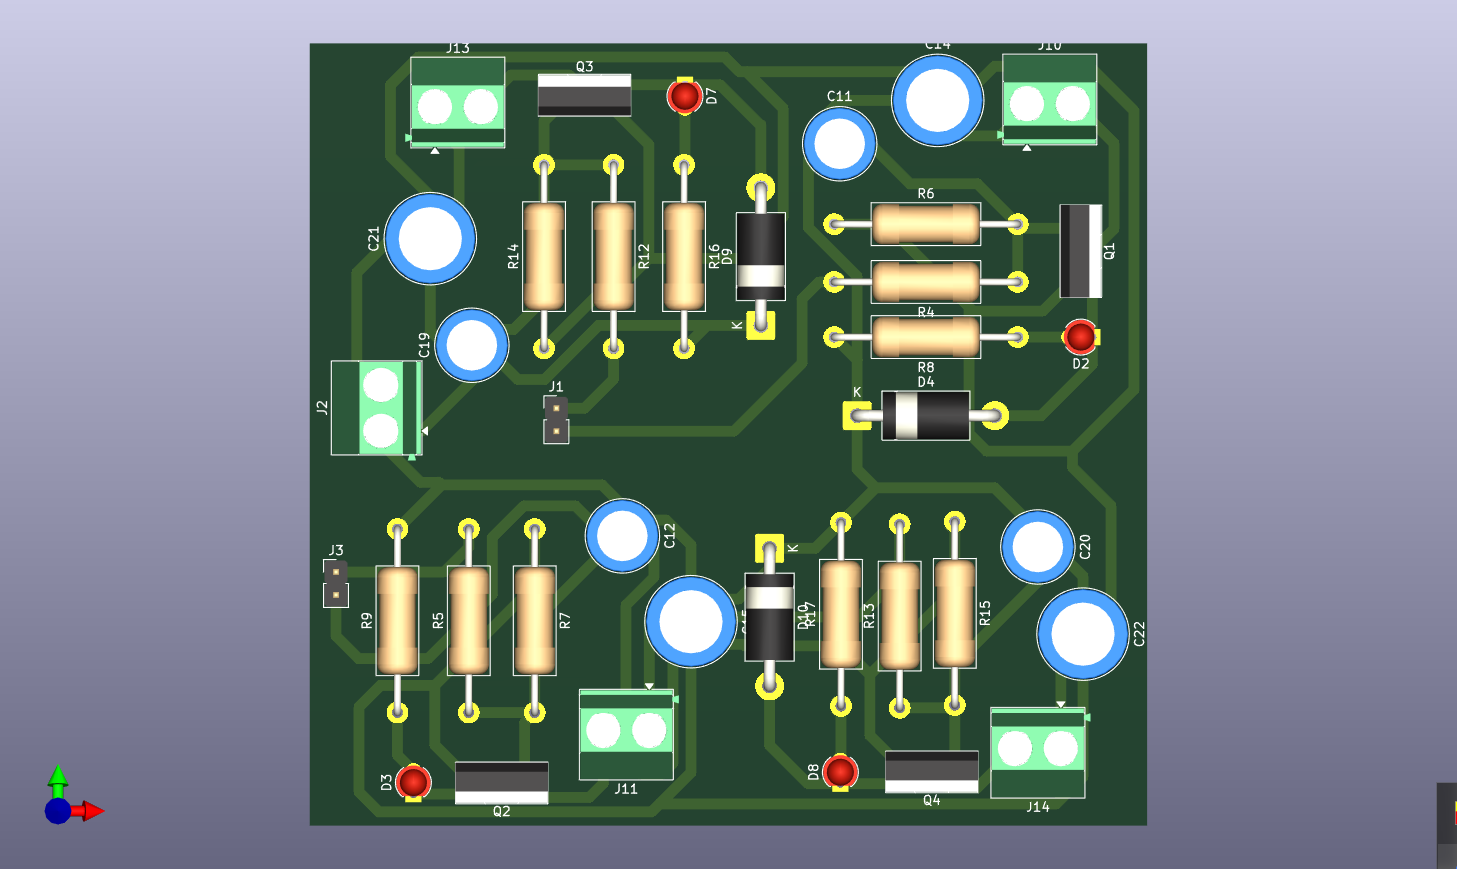
\includegraphics[width=\textwidth]{images/model3D_circuit_puissance.png}
        \caption{Modélisation 3D — Carte puissance}
        \label{fig:annexe_pcb_3d_puissance}
    \end{subfigure}
    \hfill
    \begin{subfigure}[b]{0.48\textwidth}
        \centering
        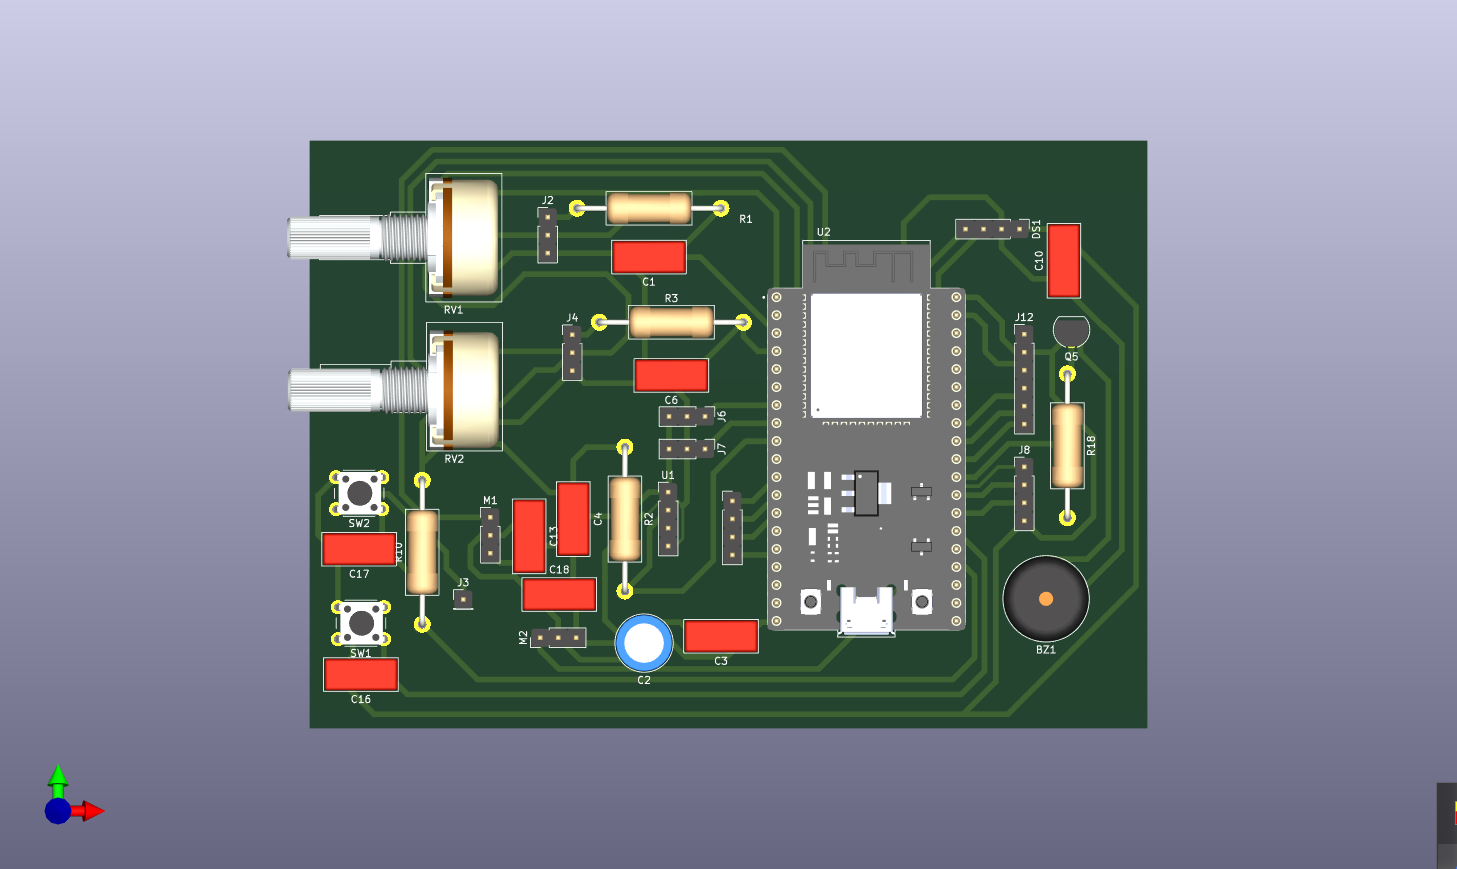
\includegraphics[width=\textwidth]{images/model3D_circuit_commande.png}
        \caption{Modélisation 3D — Carte commande}
        \label{fig:annexe_pcb_3d_commande}
    \end{subfigure}
    \vspace{0.3cm}
    \begin{subfigure}[b]{0.48\textwidth}
        \centering
        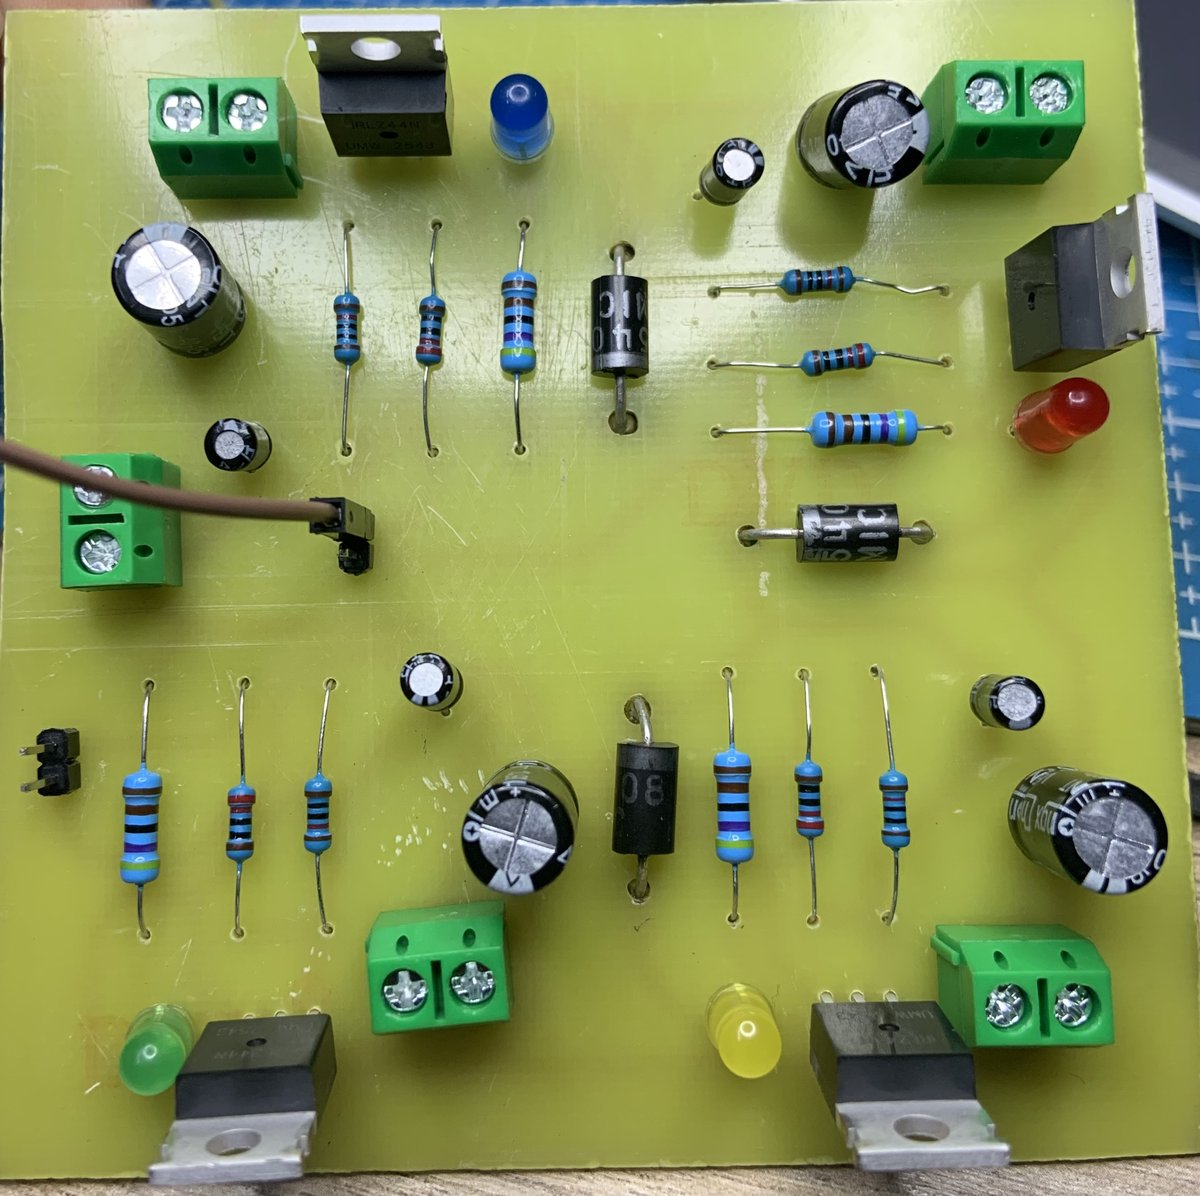
\includegraphics[width=\textwidth]{images/modelReel_circuit_puissance.jpg}
        \caption{Carte puissance réelle (assemblée)}
        \label{fig:annexe_pcb_3d_puissance_reel}
    \end{subfigure}
    \hfill
    \begin{subfigure}[b]{0.48\textwidth}
        \centering
        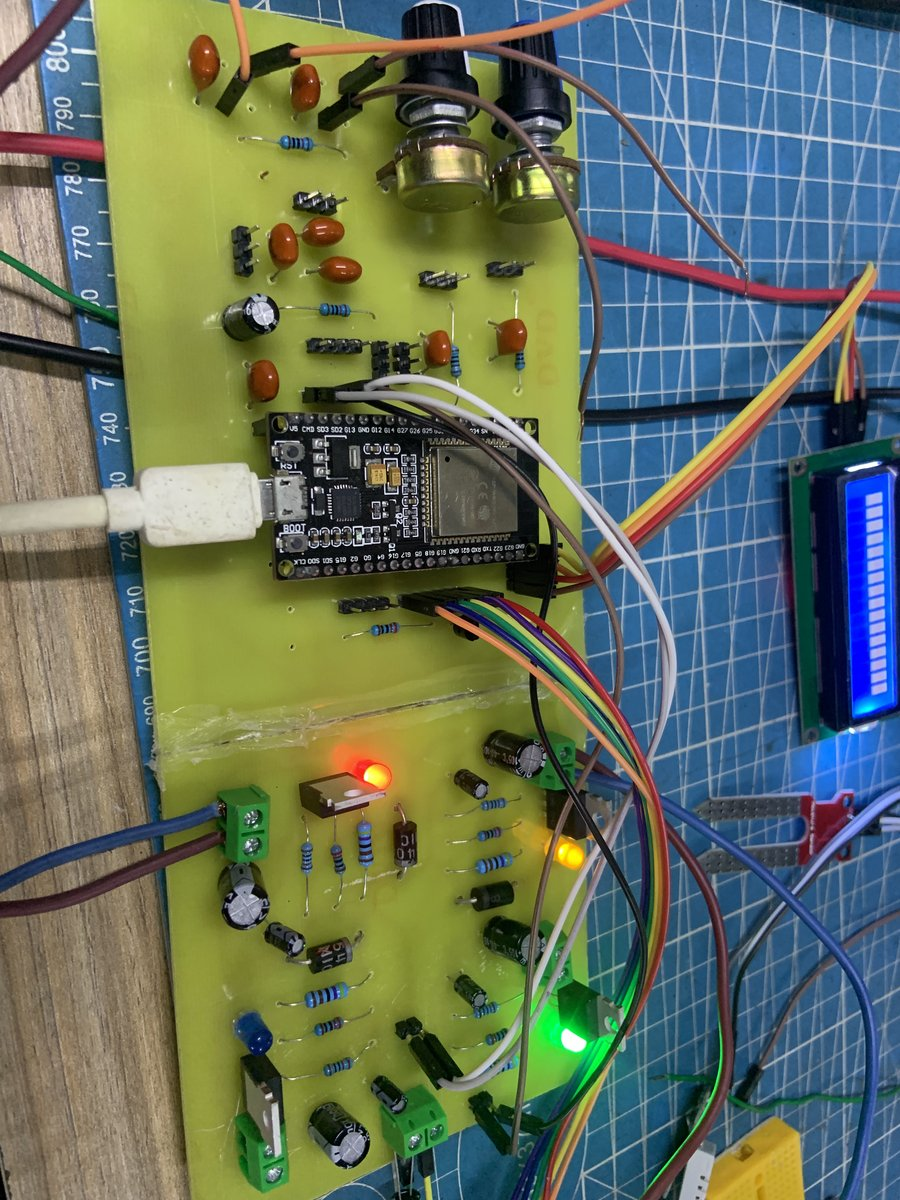
\includegraphics[width=\textwidth]{images/modelReel_circuit_commande.jpg}
        \caption{Carte commande réelle (assemblée)}
        \label{fig:annexe_pcb_3d_commande_reel}
    \end{subfigure}
    \caption{Rendus 3D et cartes réelles assemblées des PCB SMART-SOJA}
    \label{fig:annexe_pcb_3d}
\end{figure}

\newpage
\cleardoublepage
\stepcounter{chapter}
\chapter*{Annexe \thechapter{} : Synoptique de l'alimentation électrique}
\label{annexe:schema_alim}
\addcontentsline{toc}{section}{Annexe \thechapter{} : Synoptique de l'alimentation électrique}
\setcounter{figure}{0}



Cette annexe illustre la chaîne de puissance photovoltaïque du système SMART-SOJA (Figure \ref{fig:annexe_alim_solaire}). Le contrôleur \textbf{SHS 200} de Qotto intègre nativement un \textbf{BMS} (Battery Management System) qui assure la gestion de charge, la protection contre les surcharges et intègre la régulation \textbf{MPPT} pour maximiser l'énergie captée par le panneau solaire. Le bus 12~V alimente directement les charges de puissance (moteurs, ventilateur, résistance chauffante), tandis que les convertisseurs Buck LM2596 abaissent la tension à 5~V pour alimenter l'ESP32 et les capteurs.

\begin{figure}[H]
    \centering
    \resizebox{\textwidth}{!}{
    \begin{tikzpicture}[
        node distance=1.2cm and 1.5cm,
        block/.style={rectangle, draw=ucaoBlue, fill=ucaoBlue!5, text width=6.5em, text centered, rounded corners, minimum height=3em, line width=0.8pt, font=\scriptsize\bfseries},
        arrow/.style={-{Stealth}, line width=1pt, draw=ucaoBlue},
        biarrow/.style={{Stealth}-{Stealth}, line width=1pt, draw=ucaoBlue}
    ]
        % Nodes
        \node (panel)      [block]                      {Panneau\\50~W / 18~V};
        \node (controller) [block, right=of panel]      {SHS 200\\BMS + MPPT};
        \node (battery)    [block, below=of controller] {EV12-20\\12~V / 20~Ah};
        \node (buck)       [block, right=of controller] {LM2596\\12~V $\to$ 5~V};
        \node (loads12)    [block, above right=0.6cm and 1.2cm of controller]
                           {12~V — Puissance\\Moteurs, Ventil., Résist.};
        \node (loads5)     [block, right=of buck]       {5~V — Commande\\ESP32 + Capteurs};

        % Paths
        \draw [arrow]   (panel)      -- node[above, font=\tiny] {18~V DC}  (controller);
        \draw [biarrow] (controller) -- node[right, font=\tiny] {Charge/Décharge} (battery);
        \draw [arrow]   (controller) -- node[above, font=\tiny] {12~V DC}  (loads12);
        \draw [arrow]   (controller) -- node[above, font=\tiny] {12~V DC}  (buck);
        \draw [arrow]   (buck)       -- node[above, font=\tiny] {5~V DC}   (loads5);
    \end{tikzpicture}
    }
    \caption{Synoptique de la chaîne de puissance photovoltaïque SMART-SOJA}
    \label{fig:annexe_alim_solaire}
\end{figure}



\tableofcontents

\end{document}
